%%%%%%%%%%%%%%%%%%%%%%%%%%%%%%%%%%%%%%%%%%%%%%%%%%%%%%%%%%%%%%%%%%%%%%%%%%%%%%%%%%%%%%%%%%%%
%	Authors: Stracquadanio Lab
%   Manuscript version: 4.0.2-draft
%%%%%%%%%%%%%%%%%%%%%%%%%%%%%%%%%%%%%%%%%%%%%%%%%%%%%%%%%%%%%%%%%%%%%%%%%%%%%%%%%%%%%%%%%%%%

\documentclass[11pt, a4paper]{article}
\usepackage[left=2cm, right=5cm, top=2cm]{geometry}
\usepackage{helvet}
\usepackage{listings}
\usepackage{algorithmicx}
\usepackage{algorithm}
\usepackage{algpseudocode}
\usepackage{graphicx}
\usepackage{subcaption}
\usepackage{amsmath}
\usepackage{amsfonts}
\usepackage{amssymb}
\renewcommand{\familydefault}{\sfdefault}
\usepackage{fancyhdr}
\pagestyle{fancy}
\fancyhf{}
\rfoot{ Release: 3.1.0 - p. \thepage}
\renewcommand{\headrulewidth}{0pt}
\renewcommand{\footrulewidth}{1pt}
\usepackage{csvsimple}
\usepackage[pagewise]{lineno}
\linenumbers
\usepackage[backend=biber, bibencoding=utf8, sorting=none, maxnames=1, giveninits=true, doi=false, articletitle=false, style=nature, url=false]{biblatex}
\addbibresource{bibliography.bib}

\begin{document}
\title{Notebook: nanogate }
\author{ AngeloGaeta90 }
\maketitle

\tableofcontents
\clearpage
%%%%%%%%%%%%%%%%%%%%%%%%%%%%%%%%%%%%%%%%%%%%%%%%%%%%%%%%%%%%%%%%%%%%%%%%%%%%%%%%%%%%%%%%%%%%
%	INTRODUCTION
%%%%%%%%%%%%%%%%%%%%%%%%%%%%%%%%%%%%%%%%%%%%%%%%%%%%%%%%%%%%%%%%%%%%%%%%%%%%%%%%%%%%%%%%%%%%
\section{Introduction}
\subsection{Changelog}
\subsection{v0.0.0 - Initial release}
\label
script \textbf{testbeds generator.py} to generate testbeds
implemented script \path{/nanogate_project/data/utils/proto_nanogate.py} implemented applying naive algorithm

\paragraph{v0.0.1 - testbed generator output 08/11/2019}

script \path{/nanogate_project/src/nanogate_project/pre_processing/testbeds_generator.py} now generates as output
1 fasta file for all constructs, 1 fasta file for all parts , 1 .csv table to map constructs and parts

script \textbf{nanogate.py} implemented

\textbf{Snakefile} snakemake pipeline implemented

\subsection{v0.0.2 - jaccard threshold kmer length 15/11/2019}
\begin{enumerate}
        \item nanogate tool has been moved out from the repo
        \item the script \textbf{process table.py} has been implemented to process nanogate results
        \item the scripts \textbf{jaccard evaluation table.py} \\  
        and \path{/nanogate_project/src/nanogate_project/post_processing/jaccard_evaluation_table.py} \\ 
        have been implemented to create table and plot related to the jaccard threshold value
       \item the snakemake pipeline has been updated with new rules
\end{enumerate}


\subsection{0.0.3 - pipeline-fixes and poisson filter 29/11/2019}
\begin{enumerate}
\item the folder structure odf the project has been reshaped, no command line scipt is required to perform a
full analysis
\item A poisson filter has been applied to cut out reads too small
\item true and false positive and summary stats added
\end{enumerate}

\subsection{v0.0.4 - nanogate filtered and row, filter by sampling, truepositive fix 06/12/2019}
\begin{enumerate}
\item Nanogate is now split into two different methods raw and filtered:
 raw evaluates the Jaccard for each part
 filtered filter out parts on the basis of constructs length and jaccard value
\item theoretical samples are now generated by sampling and assembling parts until their average is stable
\item True positive are now evaluated per simple construct not by part
\end{enumerate}

\subsection{v0.0.5 - find kmer size given error rate, testbed similarity}
\begin{enumerate}
\item In \textbf{nanogate} the kmer length is no longer required, can be evaluated from the error rate
\item \path{testbed_generator.py} now allow to define constructs similarity, the script need reshaping though
\item Snakemake pipeline now include error rate parameter
\end{enumerate}

\subsection{v2.0.0 - runs,time plot, stats per run, cloned parts}
\begin{enumerate}
\item the pipeline now allows the execution of multiple runs
\item Cloned parts are not considered during the evaluation of the error rate
\item \path{summary_stats.txt} is now a table, called \path{run_stats.csv}
\item summary stats evaluate on all runs are now available
\end{enumerate}

\subsection{v3.1.0 - new filter method, clone list .json , error within error, mistmatch per error, short reads per error}
\begin{enumerate}
\item the distribtution of constructs did not match a poisson distribution as consenquence \\
now all values < 5 percentile of the distribution are not considered now
\item the list of clone parts included into a json file are now \\
used as input in \textbf{nanogate} \\
\item new stats after each run are now considered \\
$correct parts/all parts$,\\ 
$wrong parts/bad matches$,\\
$mismarch/bad matches$ ,\\ 
$missing parts/bad matches$ \\
\item in \textbf{nanogate} now distribution of discarded reads, accepted reads and theoreticalreads are now plotted in output
\item constrcuts with more than 10 reads and average number of reads per constructs are now considered
\end{enumerate}

\subsection{v3.1.3 - good reads analysis 31/01/2020}
\begin{enumerate}
\item The reads id taken from badreads is now in filtered nanogate results
\item The analysis of good reads per nanogate results and \textbf{accuracy} = good reads matches $:$ good reads
\item the pipeline is now too slow though, need optimisation
\item nanogate methods draft
\end{enumerate}


\subsection{v3.1.3 - 70\% identity analysis 7/02/2020}
\begin{enumerate}
\item analysis time reduced
\item plots updated to include depth paramter
\item good reads truepositive , good reads and good redas percentage plots added
\item nanogate methods draft
\end{enumerate}

\subsection{v3.2.1 - good read criteria 7/02/2020}
\begin{enumerate}
\item considering good reads reads with length at least $99\%$ of the original constrcut 
\end{enumerate}

\subsection{v.3.4.0}
\begin{enumerate}
\item minimap2 added to the pipeline
\item added script to turn alignment to csv
\item added script to process alignment results
\item added script to evalute minimap2 results  
\end{enumerate}

\subsection{v.4.0.0}
\begin{enumerate}
\item minimap2 Real time and CPU time 
\item parts in testbeds are no longer assemble at random, each part is assigned to a position before the assembly
\item added script to perform parts combinatorial assembly
\item minimap2 mapping quality analysed
\item minimap2 alignment score analysed
\item pipeline adapted to work on combinatorial assembly 
\item scripts to write comparison tables and plot implemented
\end{enumerate}

\subsection{v.4.5.0}
\begin{enumerate}
\item pipeline adapted to work with bad quality reads
\item nanogate adapted to work with bad quality reads  
\end{enumerate}


\subsection{v.4.6.0}
\begin{enumerate}
\item nanogate aggregation raw and filter nanogate are no longer divided
\item nanogate parts order with minimap2 approach for sorting parts implemented
\item nanogate analysis per constructs implemented
\item minimap2 analysis per constructs implemented
\item consufions matrix analysis for both nanogate and minimap2
\end{enumerate}

\subsection{v.5.0.0}
\begin{enumerate}
\item nanogate parts order applying mappy approach implemented
\item nanogate parts order ratio, precision and recall analysis implemented 
\item analysis of constructs with more than $10$ reads implemented
\end{enumerate}

%%%%%%%%%%%%%%%%%%%%%%%%%%%%%%%%%%%%%%%%%%%%%%%%%%%%%%%%%%%%%%%%%%%%%%%%%%%%%%%%%%%%%%%%%%%%
%	METHODS
%%%%%%%%%%%%%%%%%%%%%%%%%%%%%%%%%%%%%%%%%%%%%%%%%%%%%%%%%%%%%%%%%%%%%%%%%%%%%%%%%%%%%%%%%%%%
\section{Methods}

\subsection{Nanogate Pseudocode}
\begin{itemize}
    \item R = reads
    \item P= parts
    \item e= error rate
    \item jt= jaccard threshold
    \item pc= parts per construct
\end{itemize}

\begin{algorithm}
    \caption{Nanogate}
    \label{alg:nanogate}
    \begin{algorithmic}[1]
    \Procedure{NANOGATE}{$R, P, E, jt, pc$}
    \State $O \gets$ RAW NANOGATE($R, P, E, k, pc$)
    \State FILTER NANOGATE($O,jt$)
    \EndProcedure
    \Procedure{RAW NANOGATE} {$R, P, E, k, pc$}
    \If {E}
       \State ${K} \gets$ getkmer( $E$) \Comment{Find kmer length given error rate}
    \Else 
        \State ${K} \gets$ $k$
    \EndIf
        \State ${PH}\gets$ Initialise()\Comment{list of parts}
        \For {Pi in P} 
           \State $PHi \gets$ gethashes(Pi,K)
           \State $PH \gets$ add(PHi)
        \EndFor 
        \State $Rf \gets$ poissontest(R,pc) \Comment{given parts generate constructs length distribution, and discard all reads too short to be part of the distribution}  
        \State $O \gets$ initialise() \Comment{Initialise output}
        \For {Rfi in Rf d} \Comment{compare each read against each part and return the jaccard containment coefficient}
            \State $RHi \gets$ gethashes($RKi,K$)
            \For {part in P }
               \State $J \gets$ jaccardcontainment(PH,RHi)
               \If {$J > jt$}
                 \State $J \gets$ addtoresult(O)
                \EndIf
            \EndFor
        \EndFor
    \EndProcedure
    \P
    \Procedure{FILTER NANOGATE}{O,jt}\Comment{For each read consider only the part with the highest jaccard, and which sum is $\geq$ than read length}
    \For {Rf in O}
    \State $Rfi \gets$ jaccardfilter(O) 
    \EndFor
    \EndProcedure
    \end{algorithmic}
\end{algorithm}

\subsection{Snakemake pipeline}

%%%%%%%%%%%%%%%%%%%%%%%%%%%%%%%%%%%%%%%%%%%%%%%%%%%%%%%%%%%%%%%%%%%%%%%%%%%%%%%%%%%%%%%%%%%%
%	RESULTS
%%%%%%%%%%%%%%%%%%%%%%%%%%%%%%%%%%%%%%%%%%%%%%%%%%%%%%%%%%%%%%%%%%%%%%%%%%%%%%%%%%%%%%%%%%%%
\section{Results}
\section{V2.0.0 }
This simulation can be executed using the following snakemake config file:
  \begin{lstlisting}[language=Python]
project: "test"
genbank: "yeast_chromosome_xiv.gb"
run: 10

generate_testbeds:
    cds_number : 50
    constructs_number: [10,50,100]
    parts : [5,10,20]
    clone_parts_amount : 0.4
    parts_similarity : 0.7

badreads:
    quantity : "50x"
    error_model: "nanopore"
    qscore_model: "nanopore"
    glitches: "0,0,0"
    junk_reads: 0
    random_reads: 0
    chimeras: 0
    identity: 95,100,4
    start_adapter_seq: ' "" '
    end_adapter_seq: ' "" '

nanogate:
     error_rate : ["001","010","030"]
     jaccard_thresholds: ["00", "01", "02", "03", "04",
     "05", "06", "07", "08", "09", "10"]

  
\end{lstlisting}

\subsection{True positive }
 \begin{figure}[ht]
      \begin{center}
      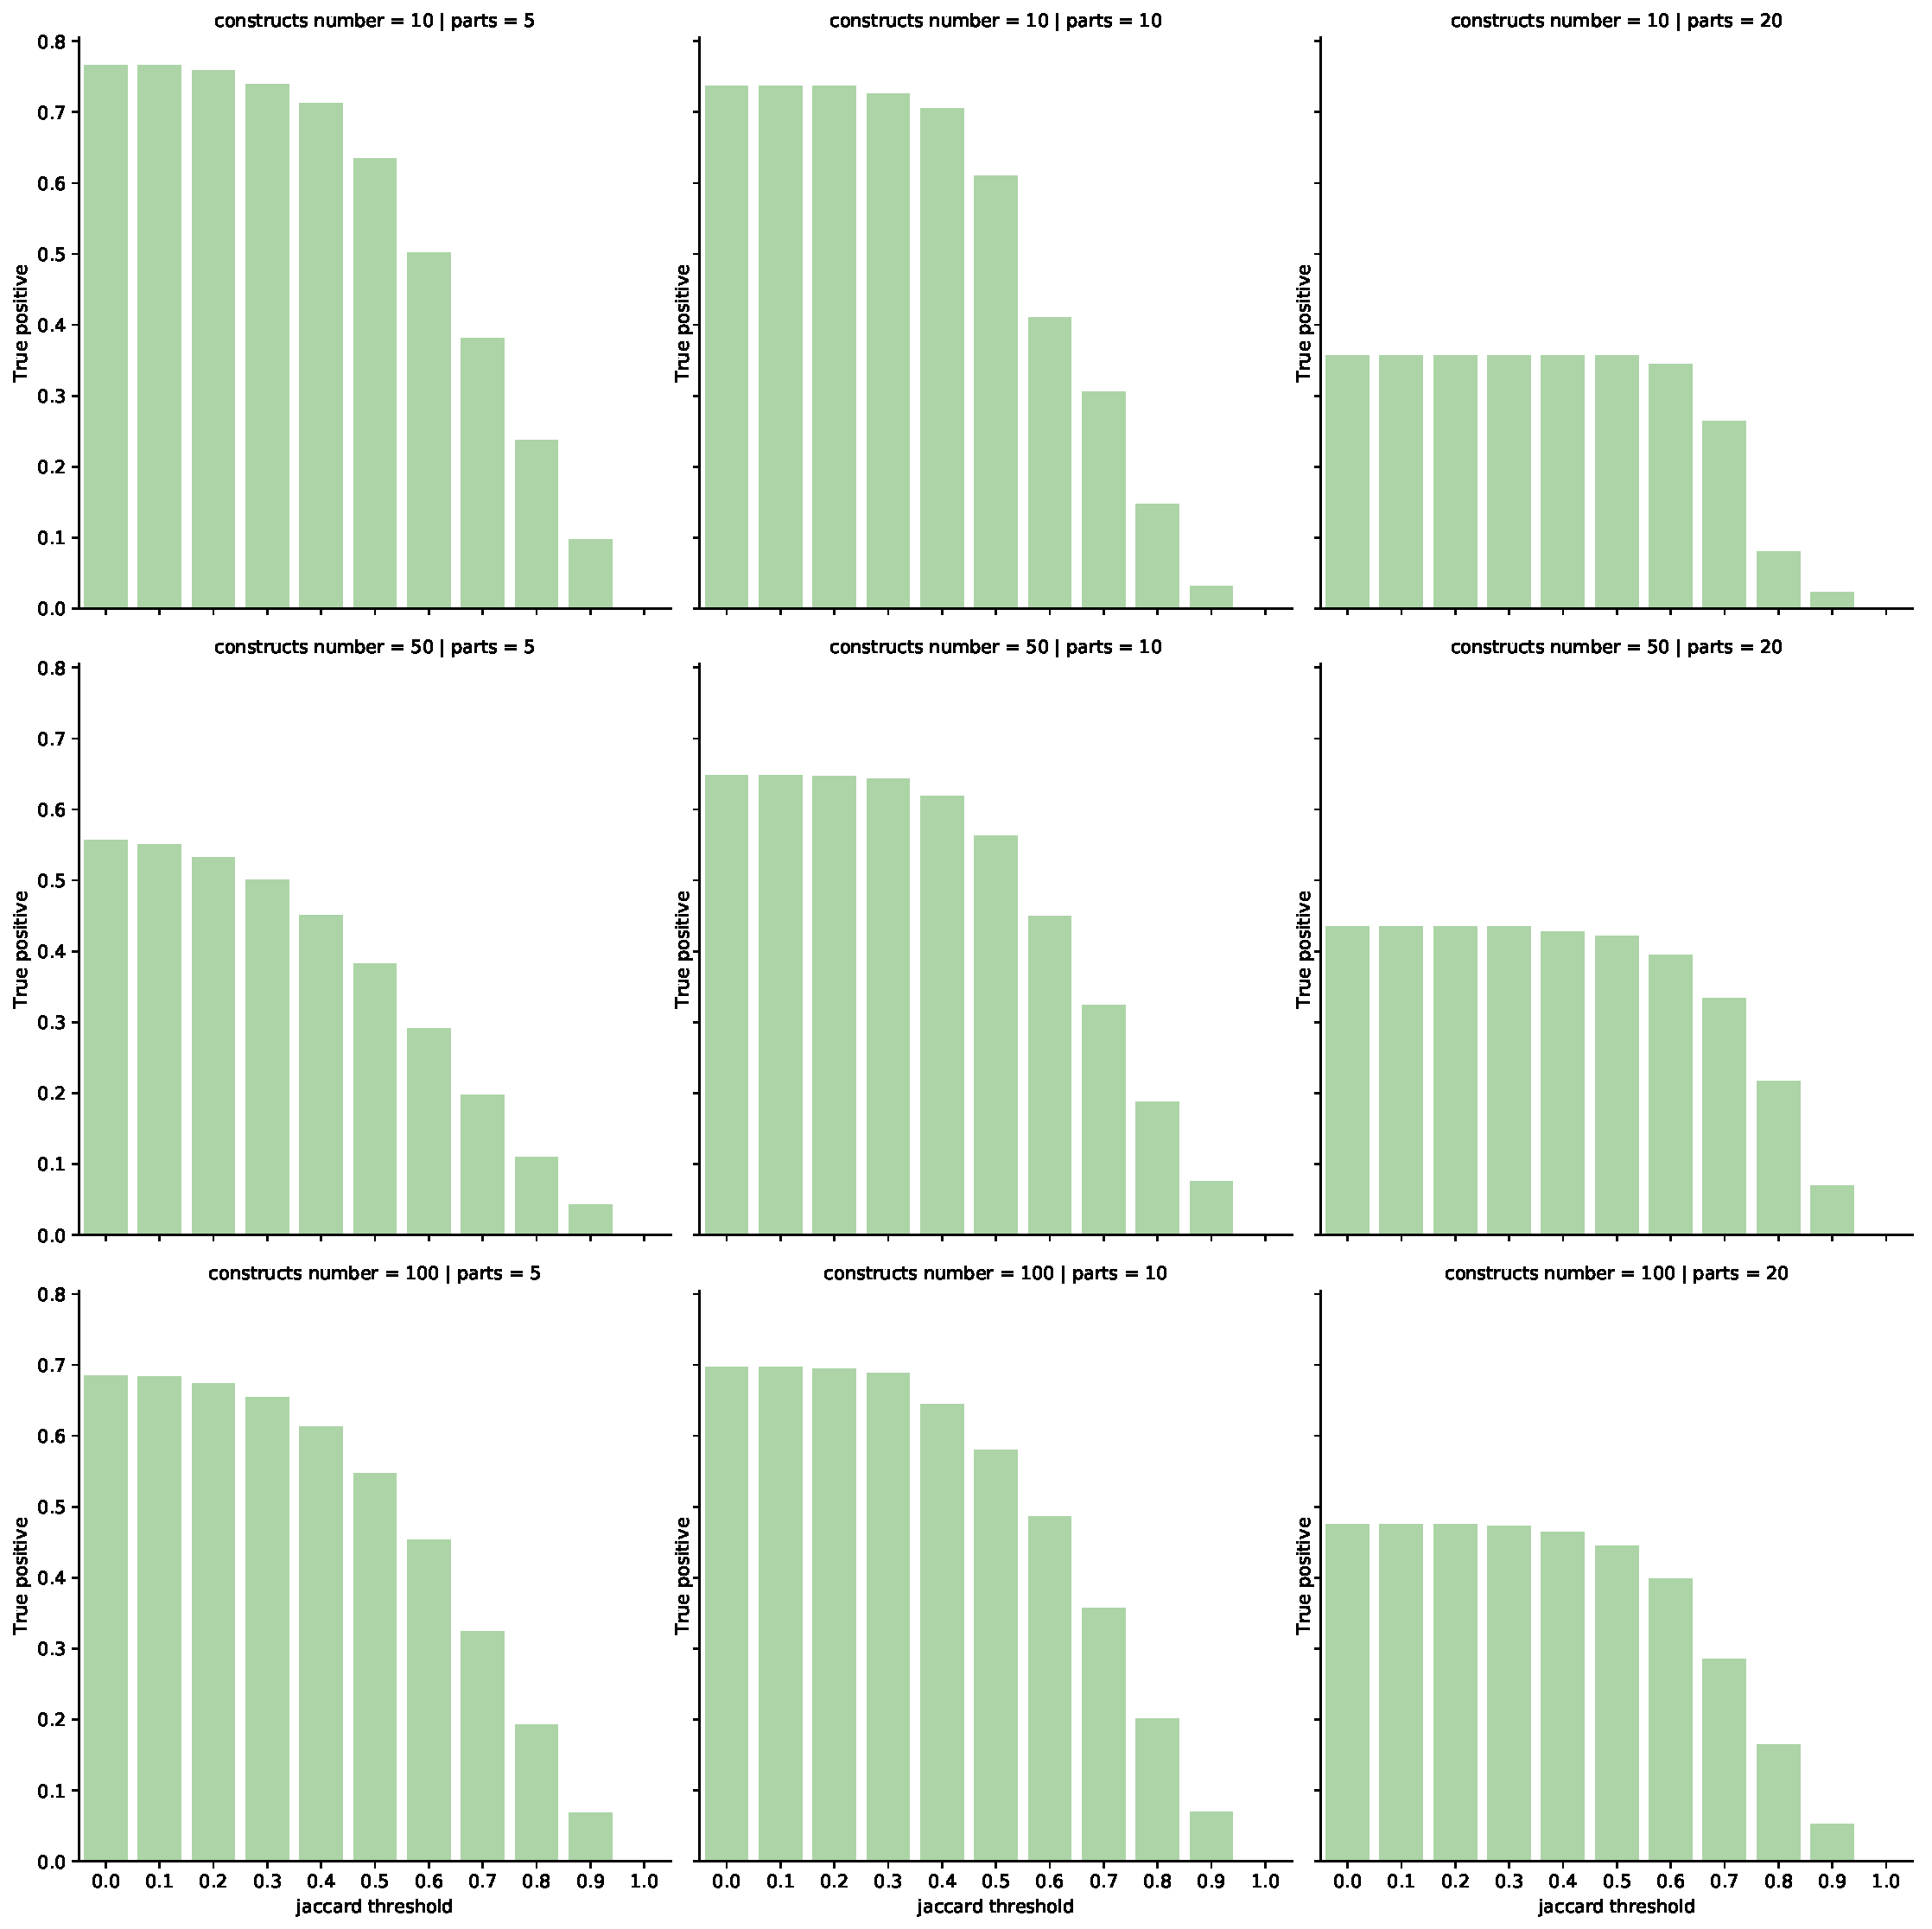
\includegraphics[width=1\textwidth]{../results/images_notebook/v_006/001_true_positive.pdf}
      \end{center}
      \caption{{\bf 001 Error rate run 0. }}
     \label{fig:v_006_001}
 \end{figure}
 
  \begin{figure}[ht]
      \begin{center}
     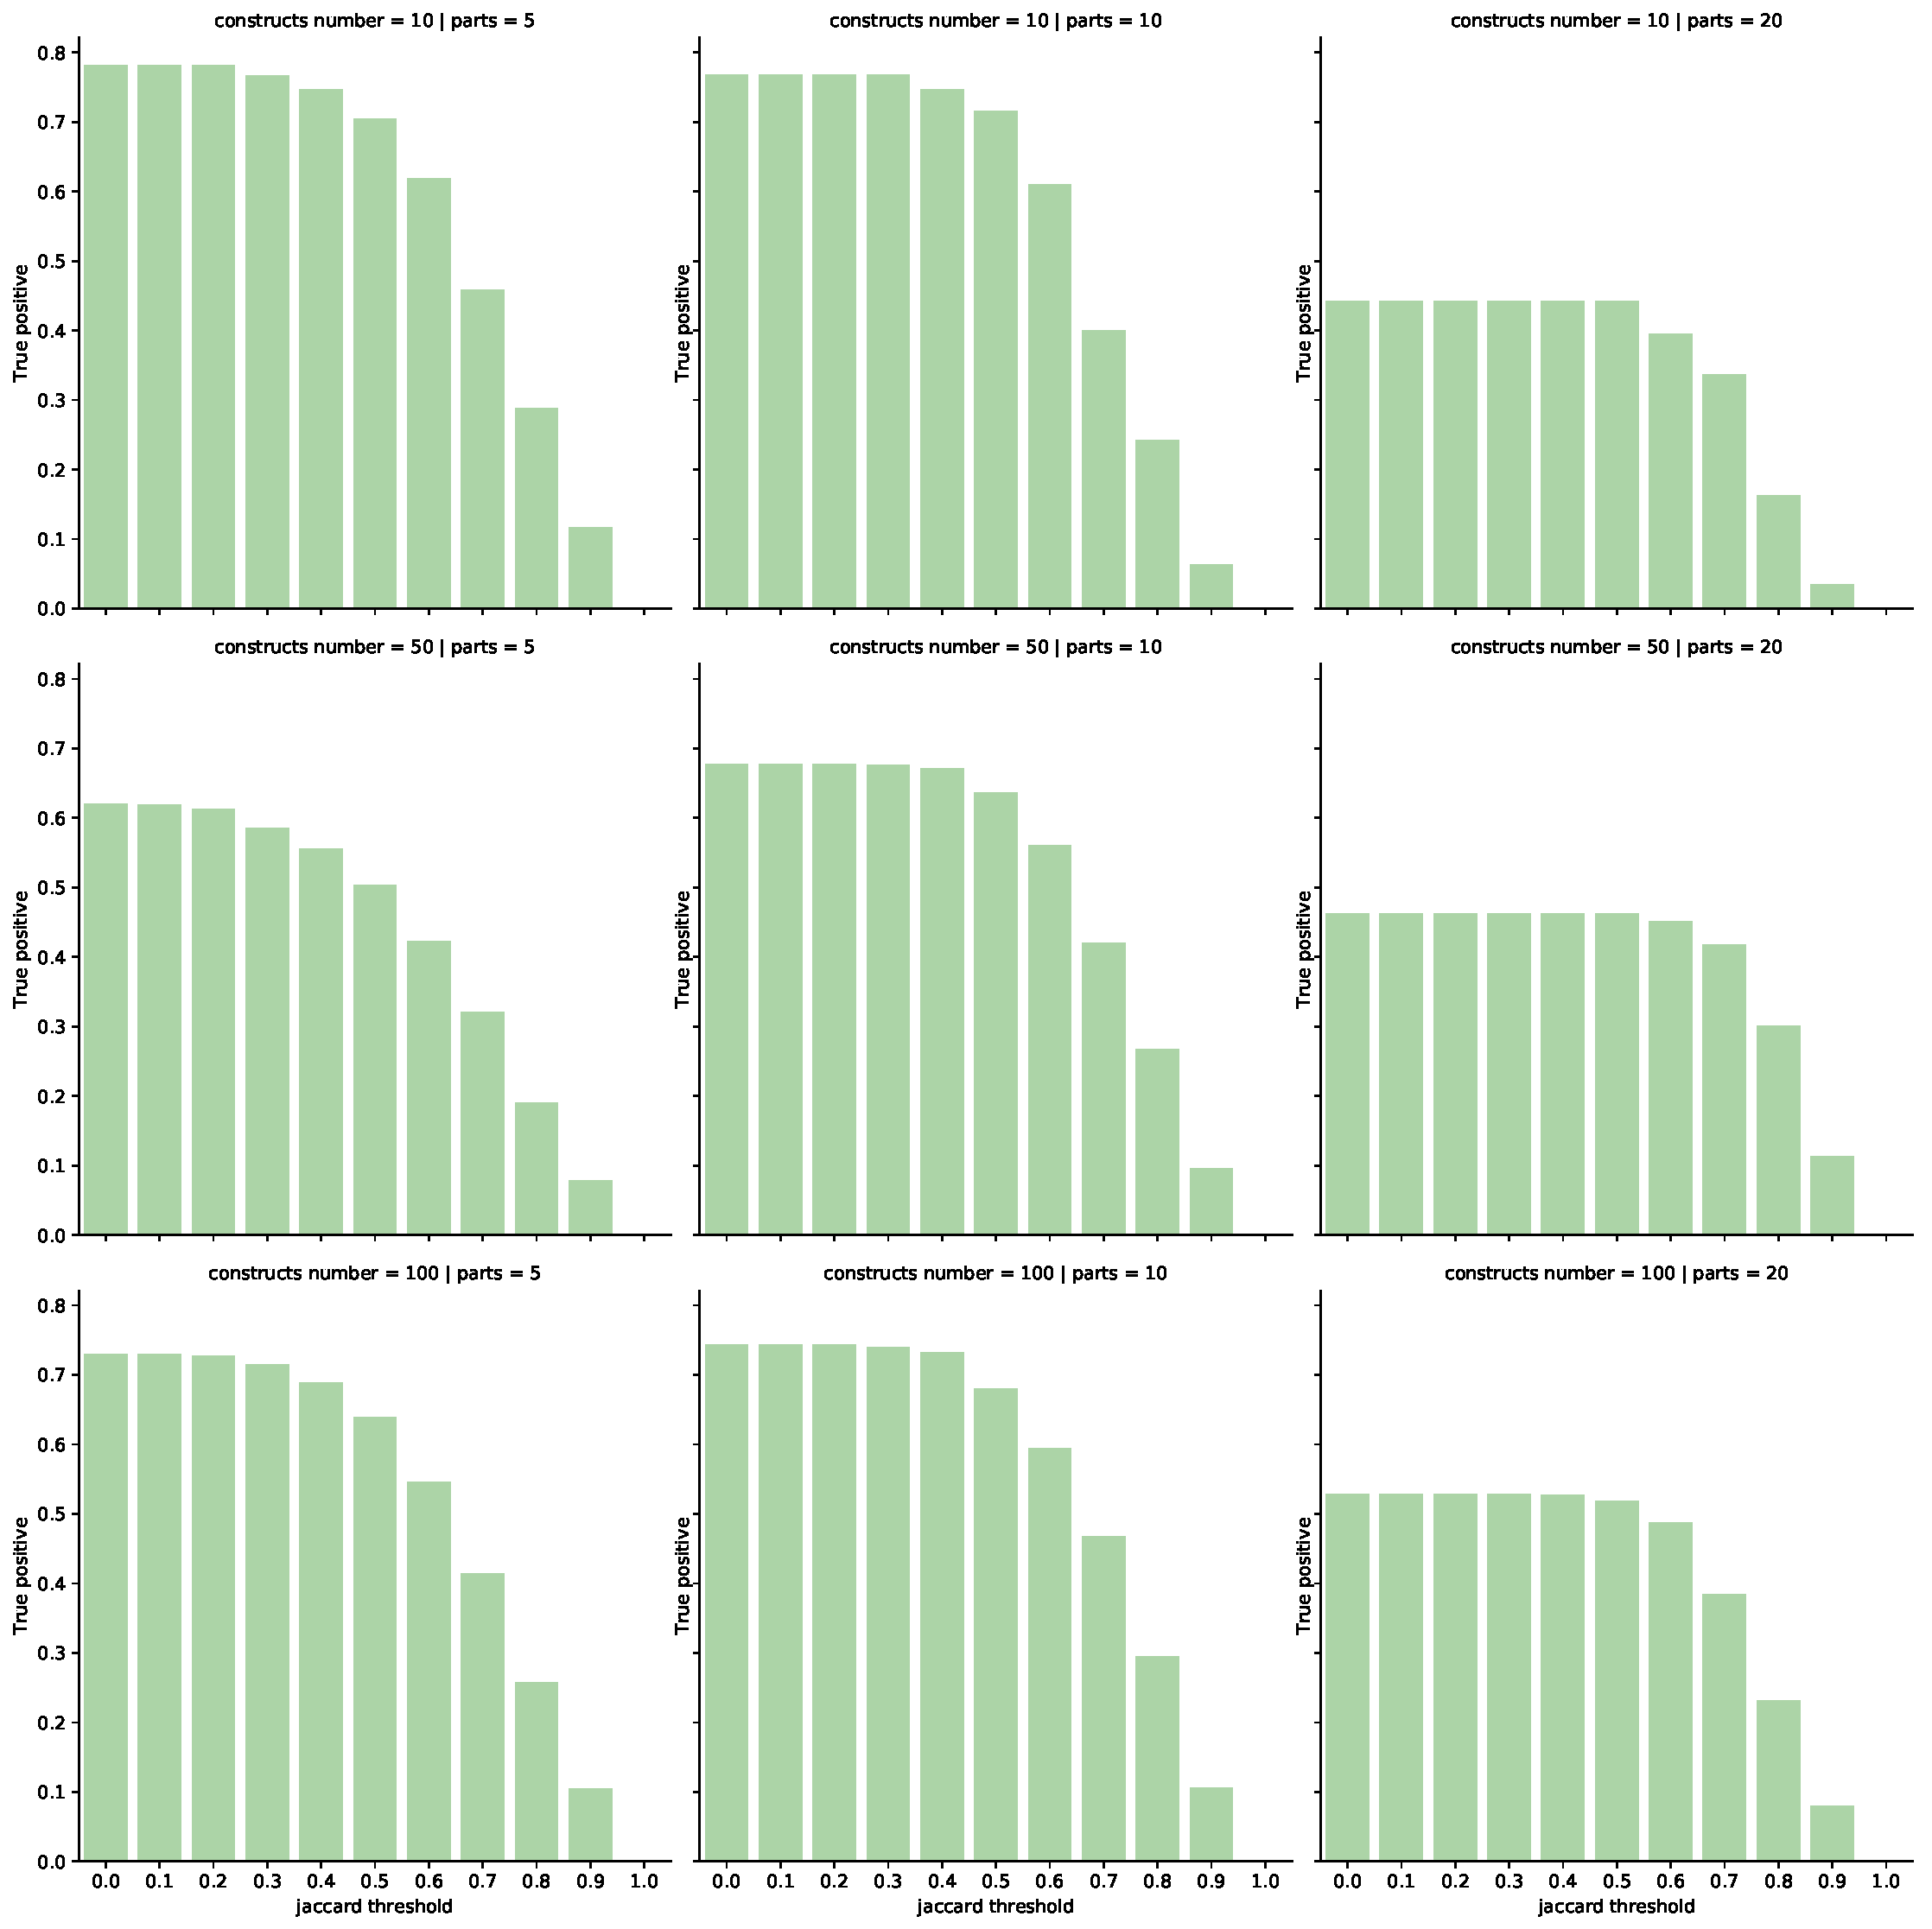
\includegraphics[width=1\textwidth]{../results/images_notebook/v_006/010_true_positive.pdf}
     \end{center}
      \caption{{\bf 010 Error rate run 0. }}
     \label{fig:V_006_010}
 \end{figure}
 
   \begin{figure}[ht]
      \begin{center}
     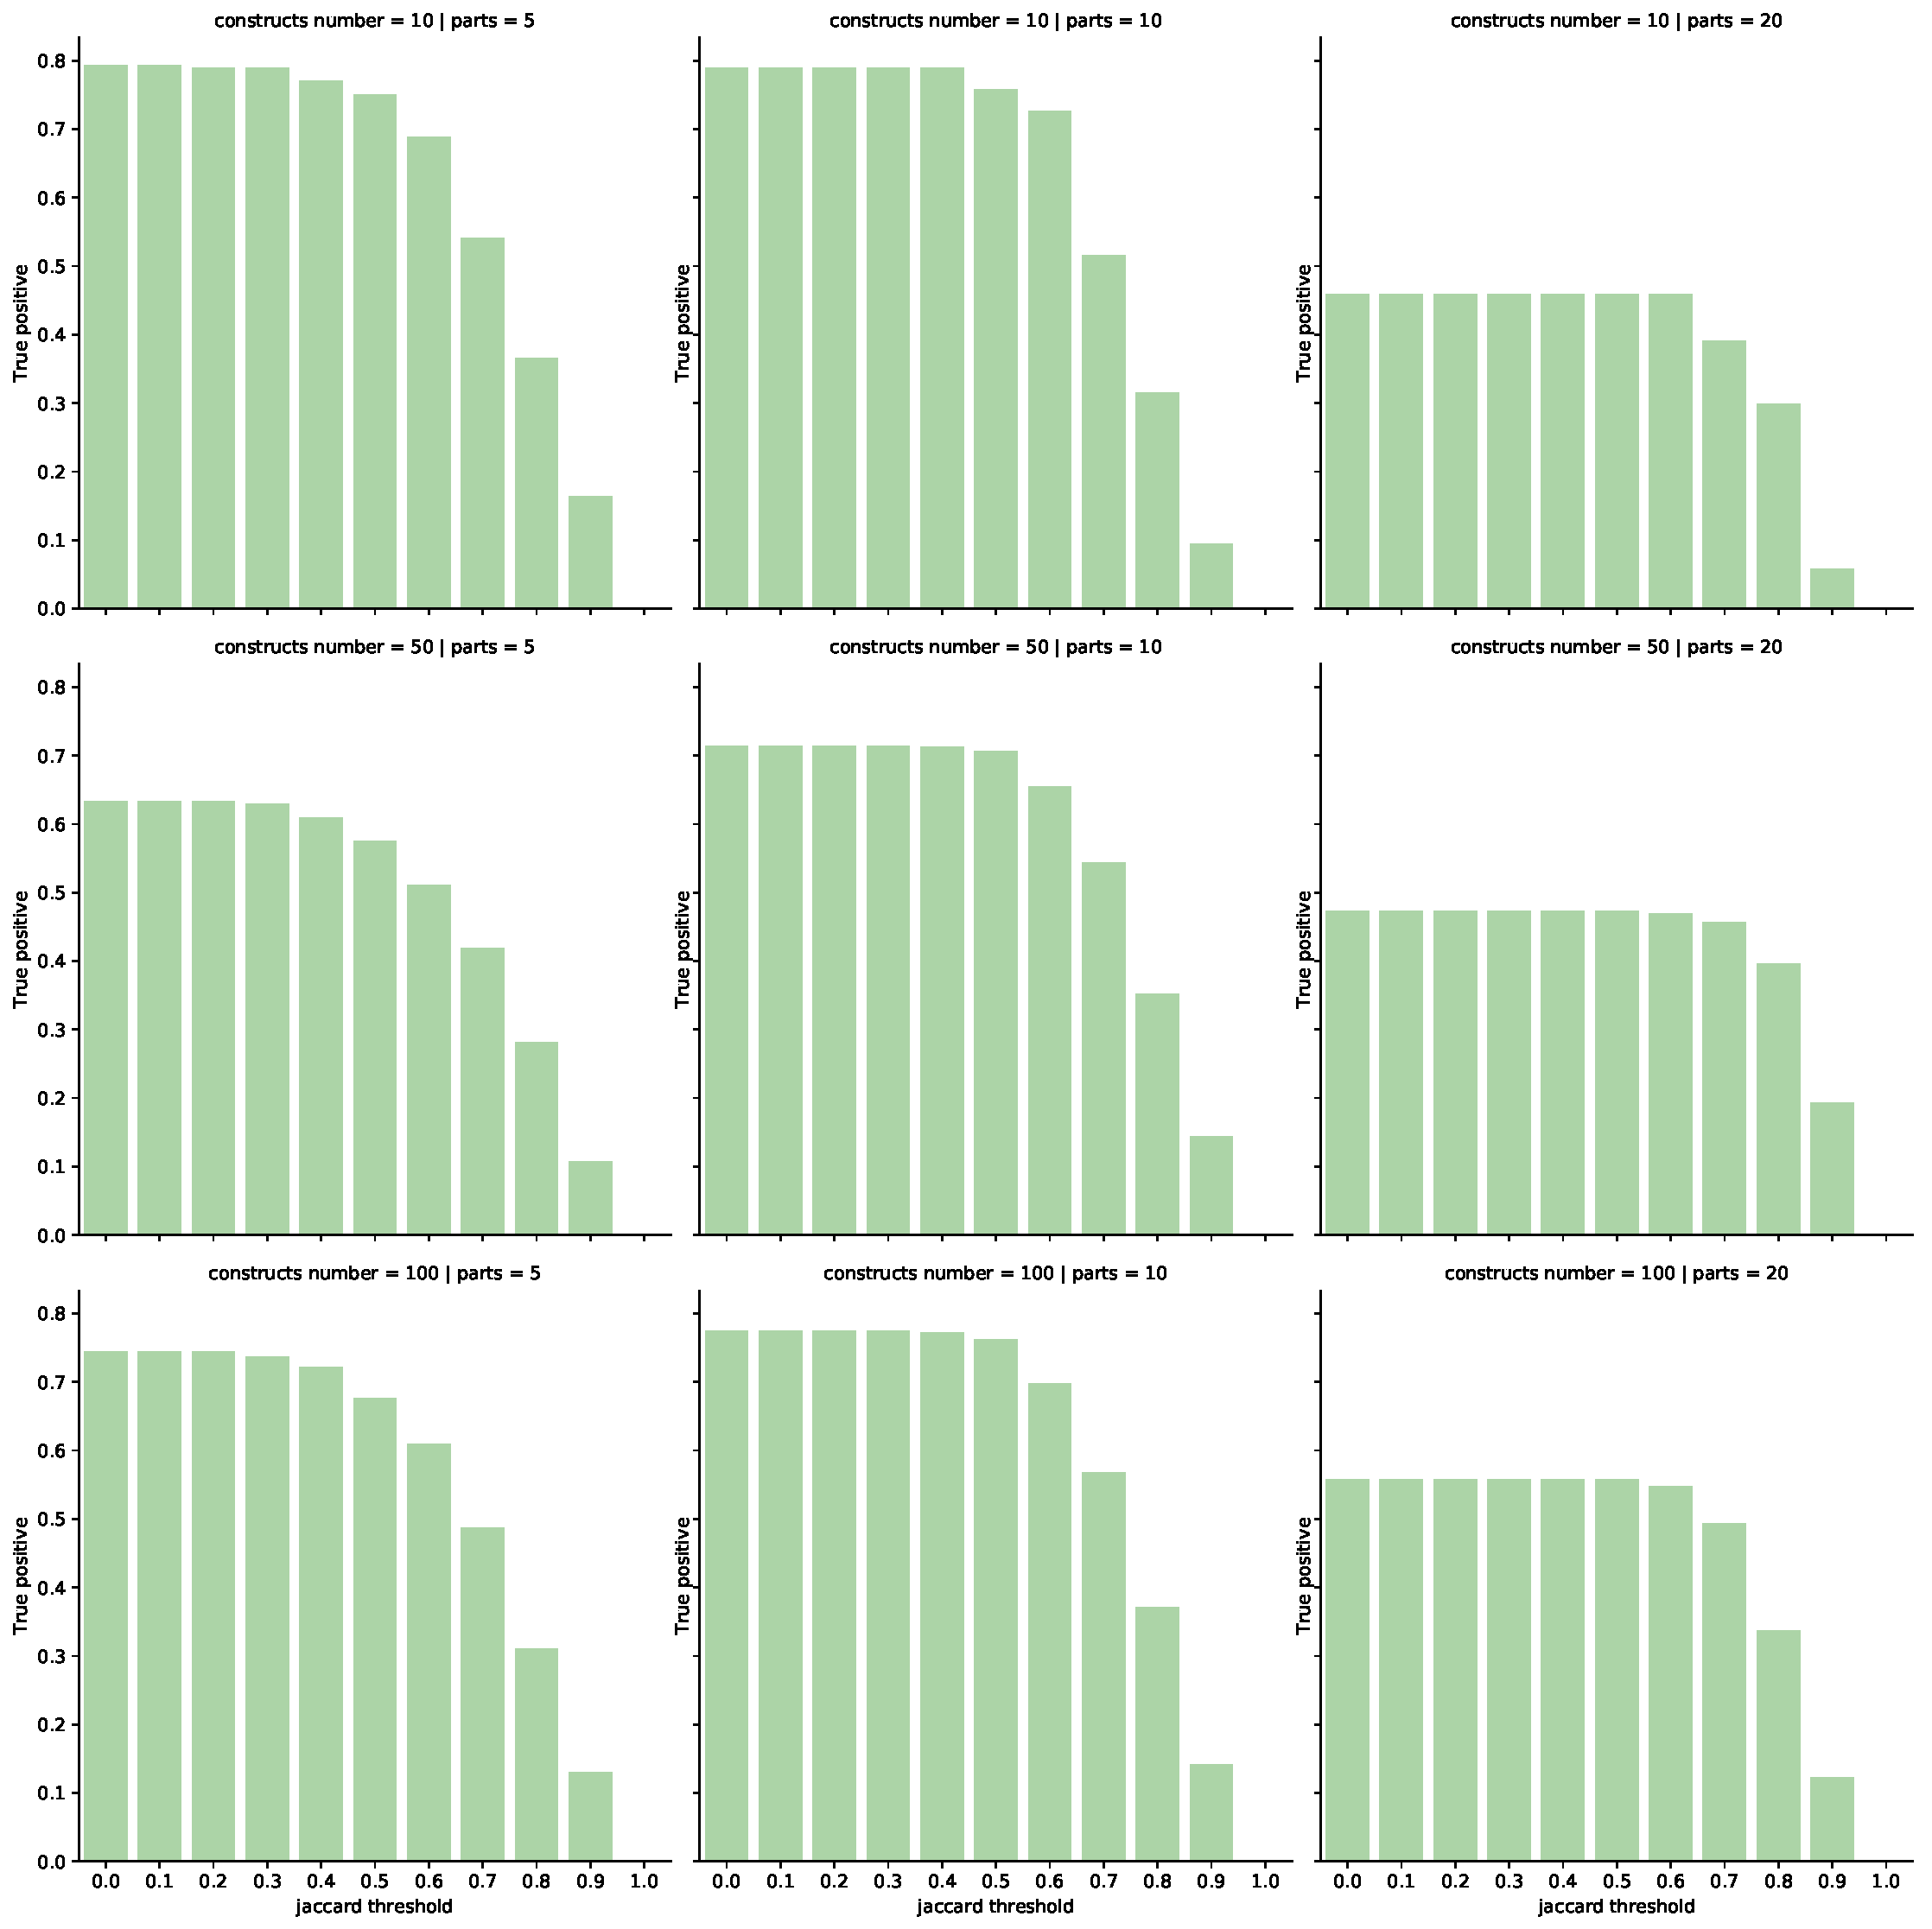
\includegraphics[width=1\textwidth]{../results/images_notebook/v_006/030_true_positive.pdf}
     \end{center}
      \caption{{\bf 030 Error rate run 0. }}
     \label{fig:V_006_030}
 \end{figure}
 
 \subsection{Time plot}
  \begin{figure}[ht]
      \begin{center}
     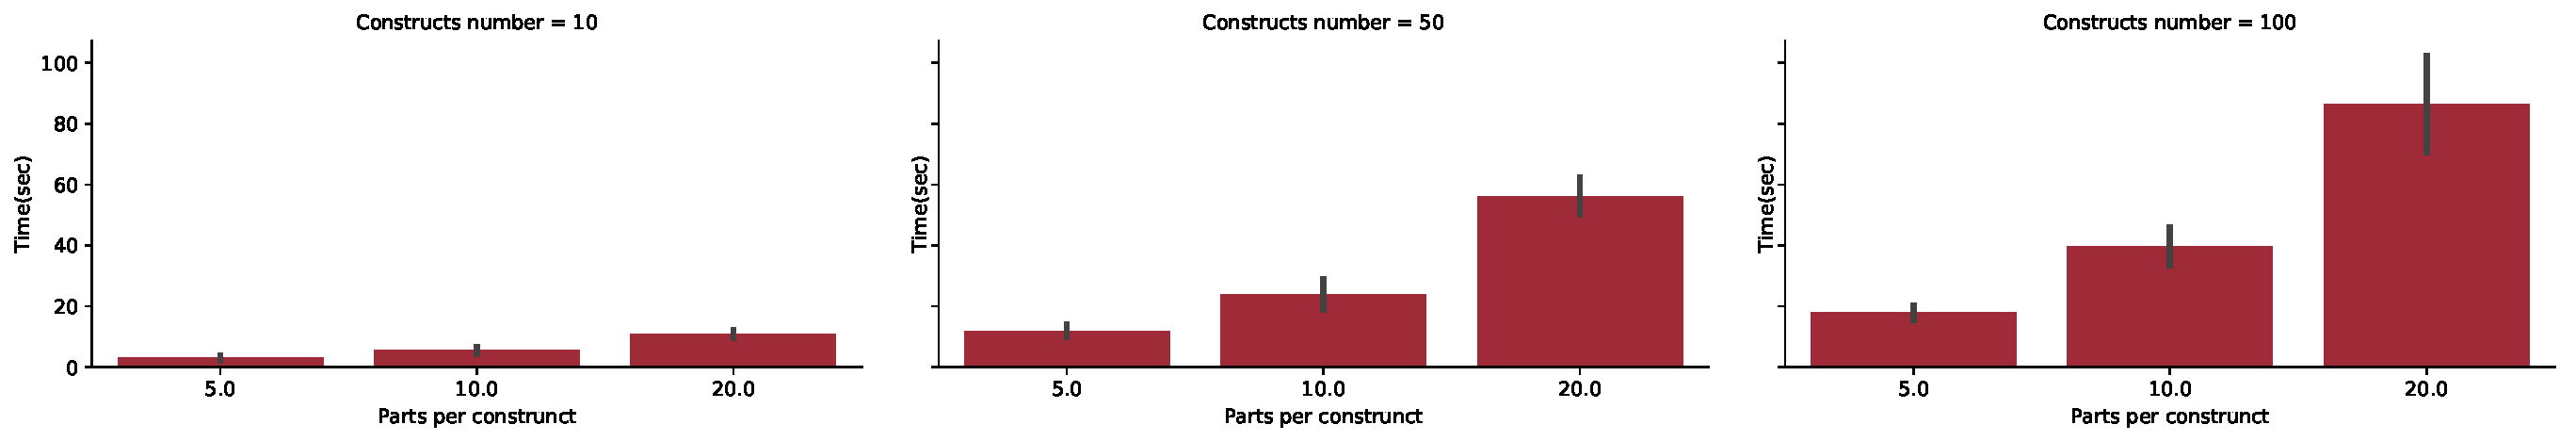
\includegraphics[width=1\textwidth]{../results/images_notebook/v_006/time_plot.pdf}
     \end{center}
      \caption{{\bf Time plot }}
     \label{fig:v_006_time_plot}
 \end{figure}



\section{Results}
\subsection{V3.1.0 }
This simulation can be executed using the following snakemake config file:
  \begin{lstlisting}[language=Python]
project: "percentile_5"
genbank: "yeast_chromosome_xiv.gb"
run: 10

generate_testbeds:
    cds_number : 50
    constructs_number: [10,50,100]
    parts : [5,10,20]
    clone_parts_amount : 0.4
    parts_similarity : 0.7

badreads:
    quantity : "50x"
    error_model: "nanopore"
    qscore_model: "nanopore"
    glitches: "0,0,0"
    junk_reads: 0
    random_reads: 0
    chimeras: 0
    identity: 95,100,4
    start_adapter_seq: ' "" '
    end_adapter_seq: ' "" '

nanogate:
     error_rate : ["001","010","030"]
     jaccard_thresholds: ["00", "01", "02", "03", "04",
      "05", "06", "07", "08", "09", "10"]

\end{lstlisting}


\subsubsection{Reads distribtution }
 \begin{figure}[ht]
      \begin{center}
      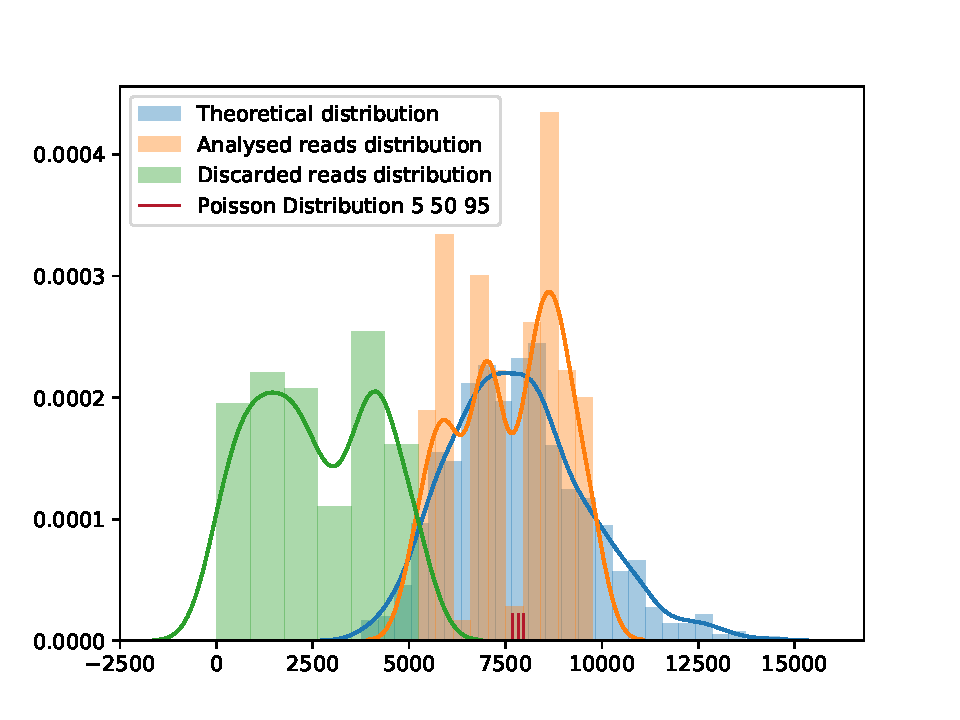
\includegraphics[width=1\textwidth]{../results/images_notebook/v_310/5_parts_distribution.pdf}
      \end{center}
      \caption{{\bf 5 parts reads distribution, the accepted reads now fits the theoretical distribution. }}
     \label{fig:v_310_reads_5_parts}
 \end{figure}
 
 \begin{figure}[ht]
    \begin{center}
    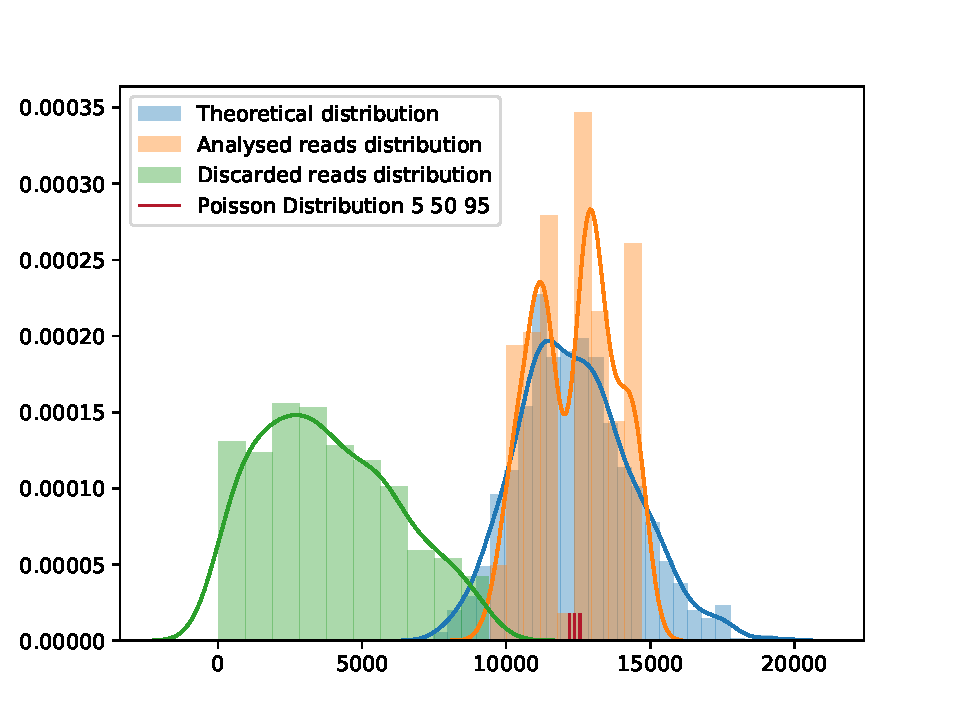
\includegraphics[width=1\textwidth]{../results/images_notebook/v_310/10_parts_distribution.pdf}
    \end{center}
    \caption{{\bf 10 parts reads distribution, the accepted reads now fits the theoretical distribution. }}
   \label{fig:v_310_reads_10_parts}
\end{figure}

\begin{figure}[ht]
    \begin{center}
    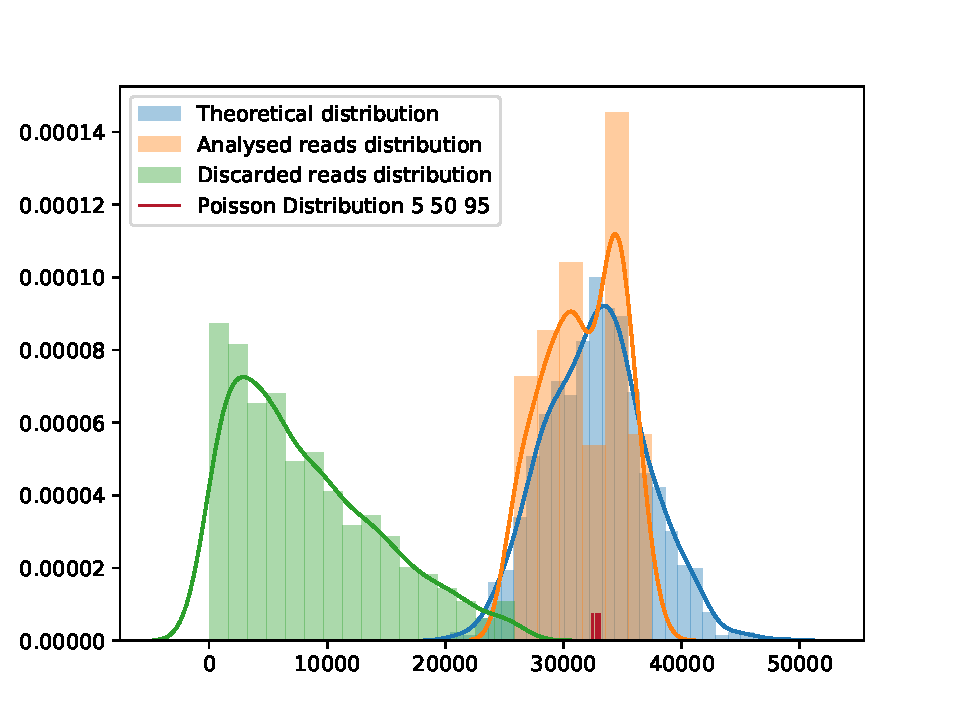
\includegraphics[width=1\textwidth]{../results/images_notebook/v_310/20_parts_distribution.pdf}
    \end{center}
    \caption{{\bf 20 parts reads distribution, the accepted reads now fits the theoretical distribution. }}
   \label{fig:v_310_reads_20_parts}
\end{figure}

 
\subsubsection{Error within error }

\begin{figure}[ht]
    \begin{center}
    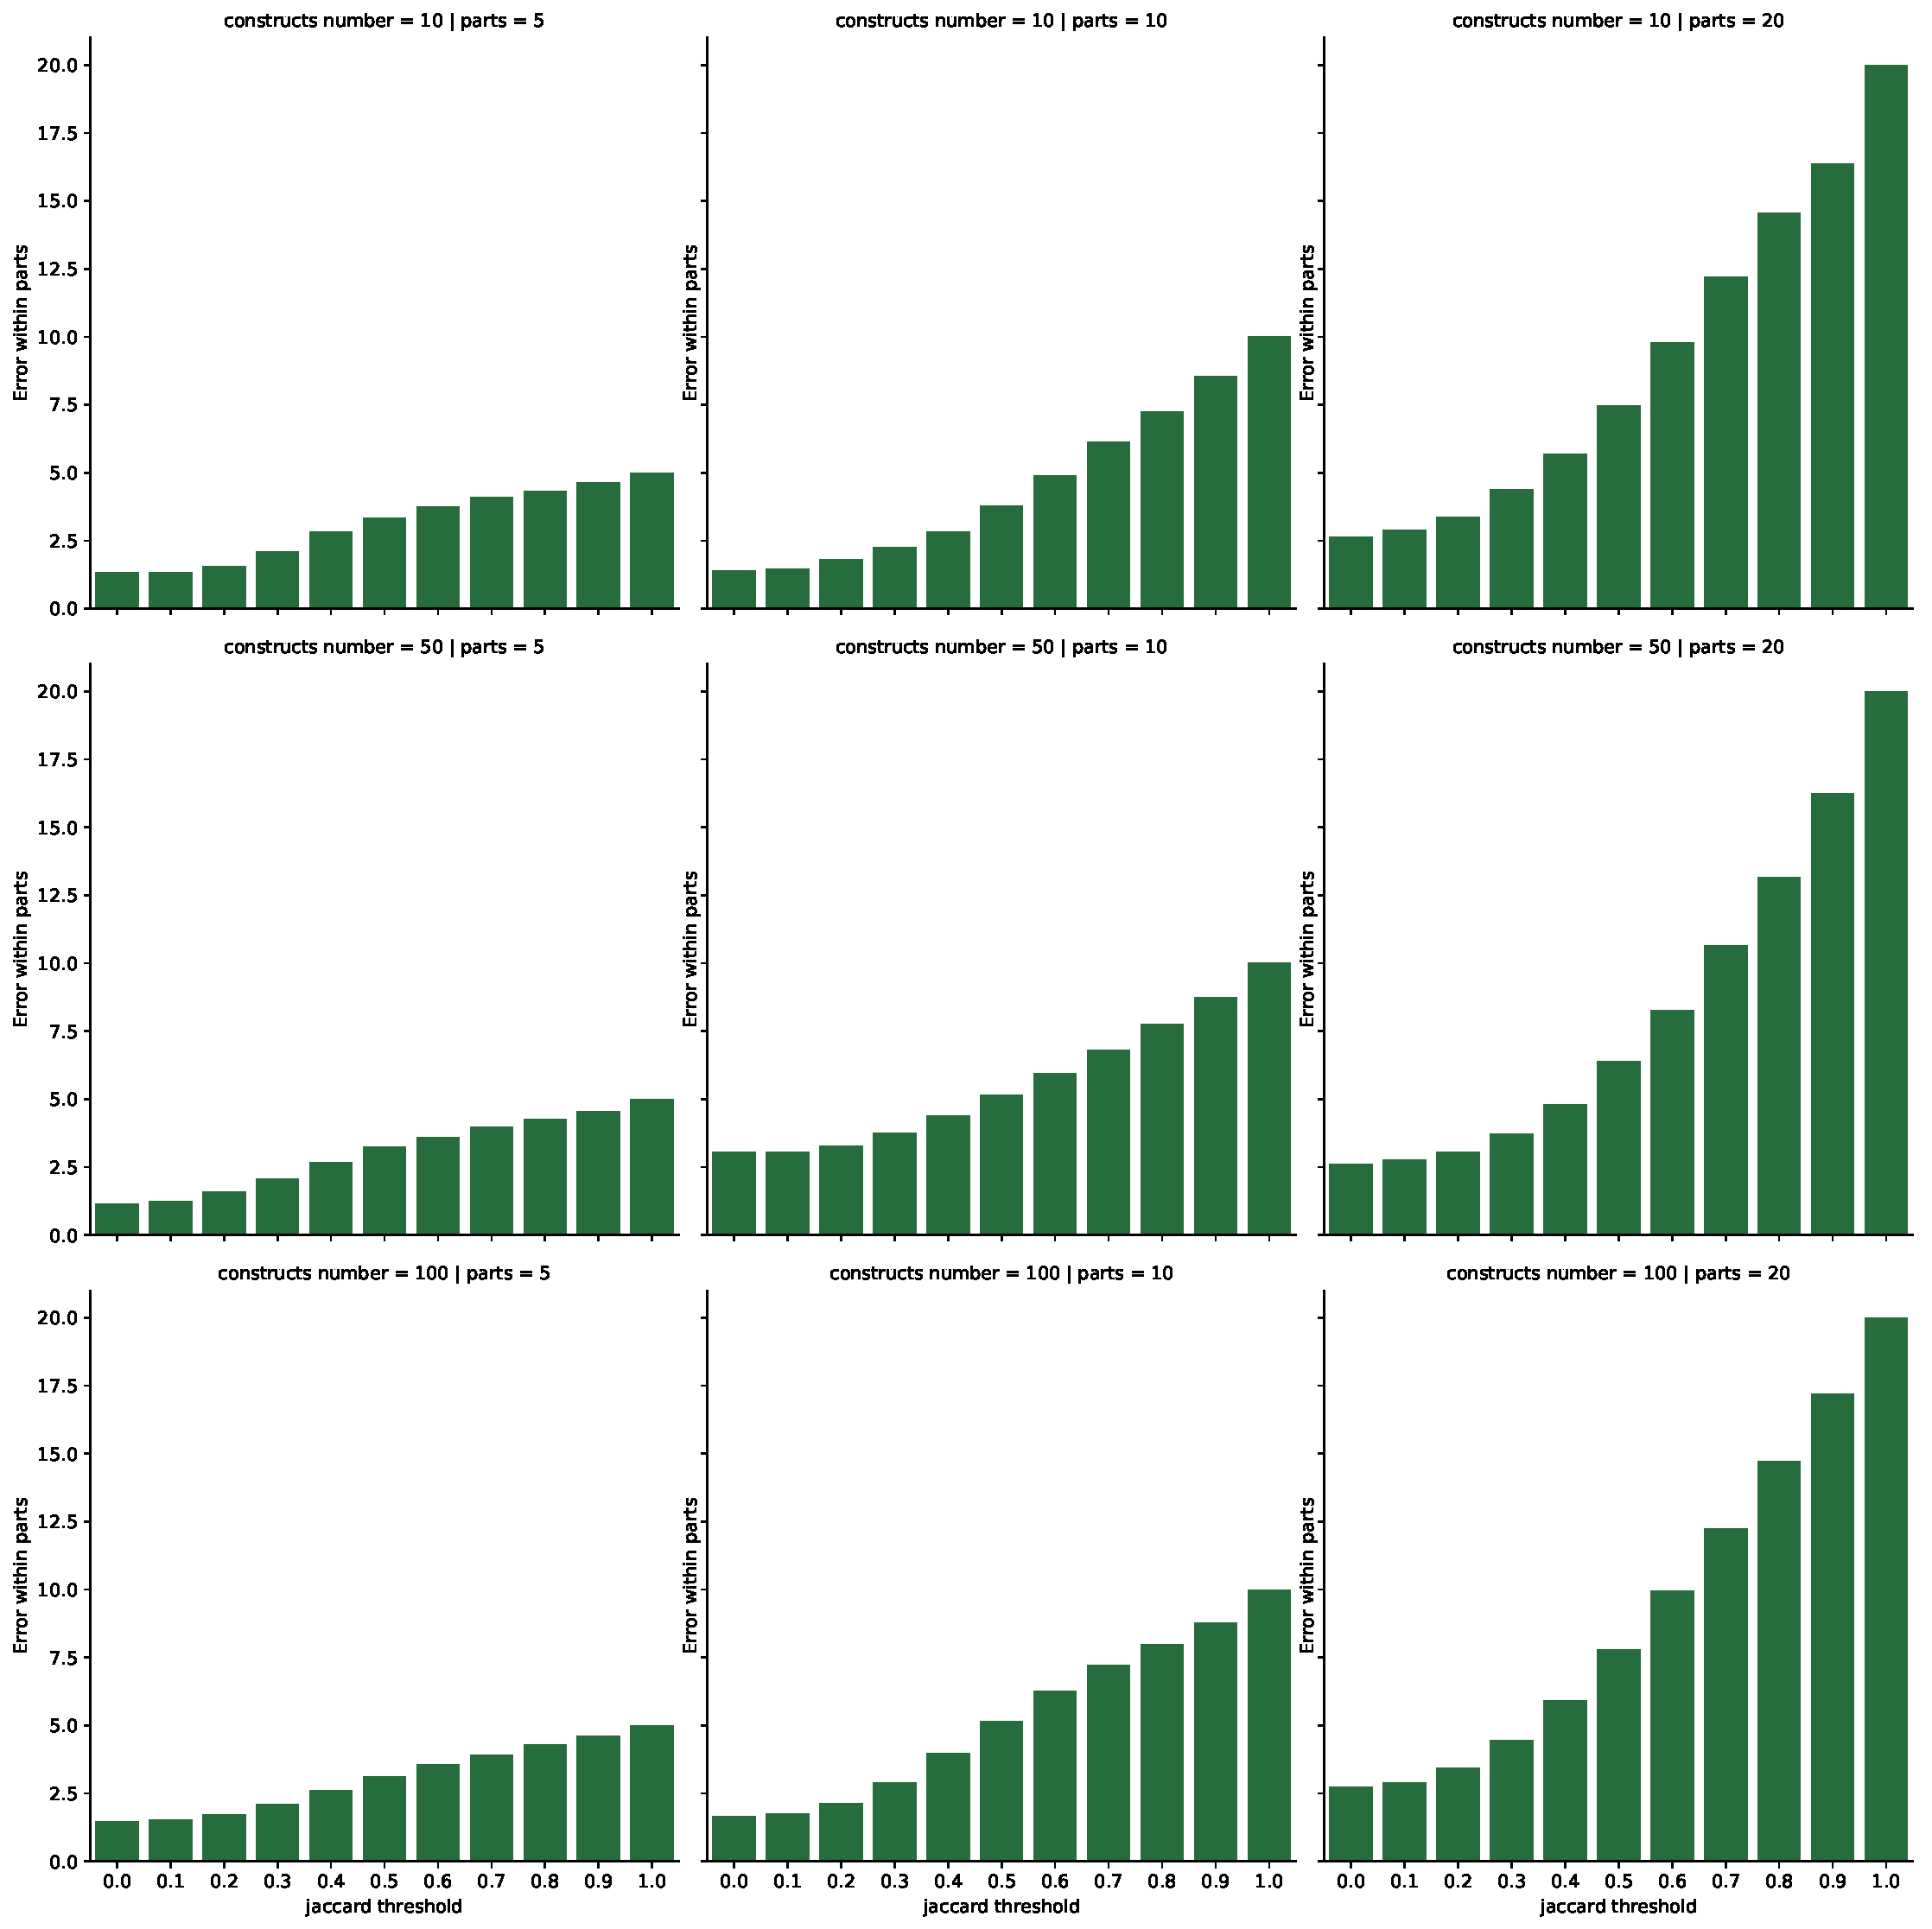
\includegraphics[width=1\textwidth]{../results/images_notebook/v_310/001_error_per_error.pdf}
    \end{center}
    \caption{{\bf Example of a Error within error plot taken from run 0.This metric is measured as $missing or wrong parts/bad matches$ }}
   \label{fig:v_310_error_within_error}
\end{figure}


\subsubsection{mismatch per error }

\begin{figure}[ht]
    \begin{center}
    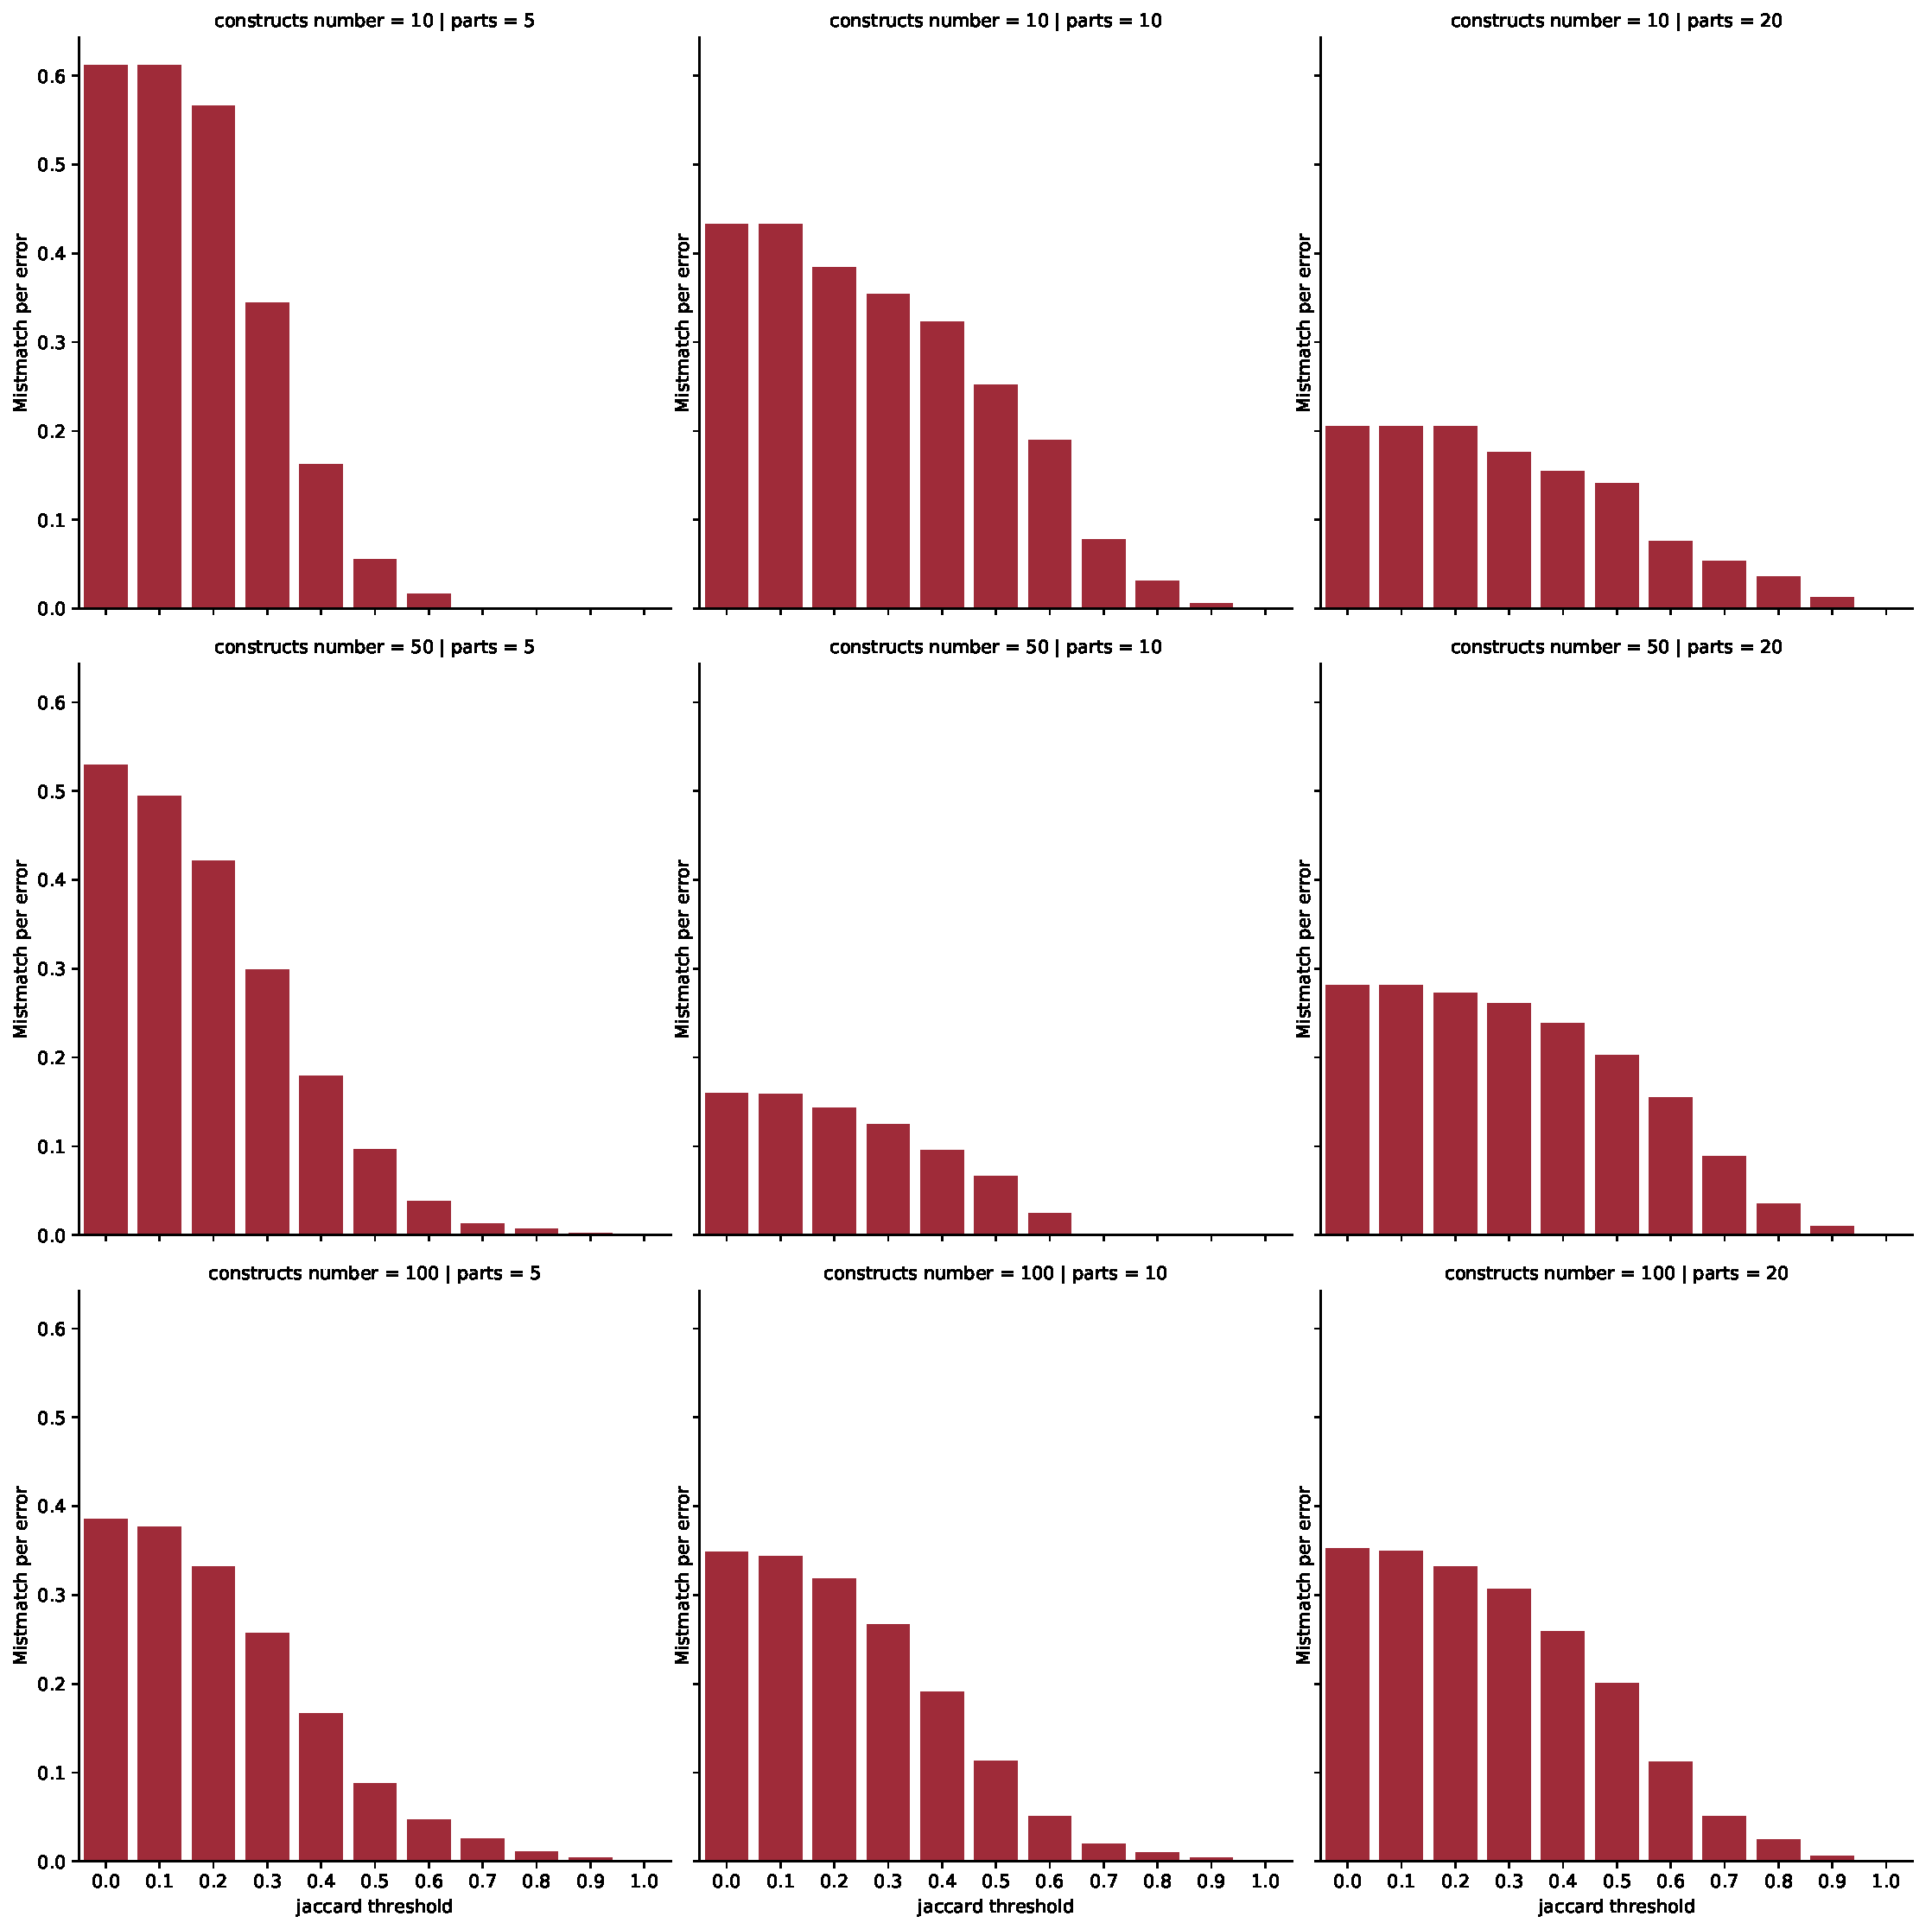
\includegraphics[width=1\textwidth]{../results/images_notebook/v_310/001_mismatch_per_error.pdf}
    \end{center}
    \caption{{\bf Example of a mismatch per error plot taken from run 0. This metric is measured as $reads with wrong parts/bad matches$ }}
   \label{fig:v_310_mismatch_per_error}
\end{figure}


\subsubsection{short read per error }

\begin{figure}[ht]
    \begin{center}
    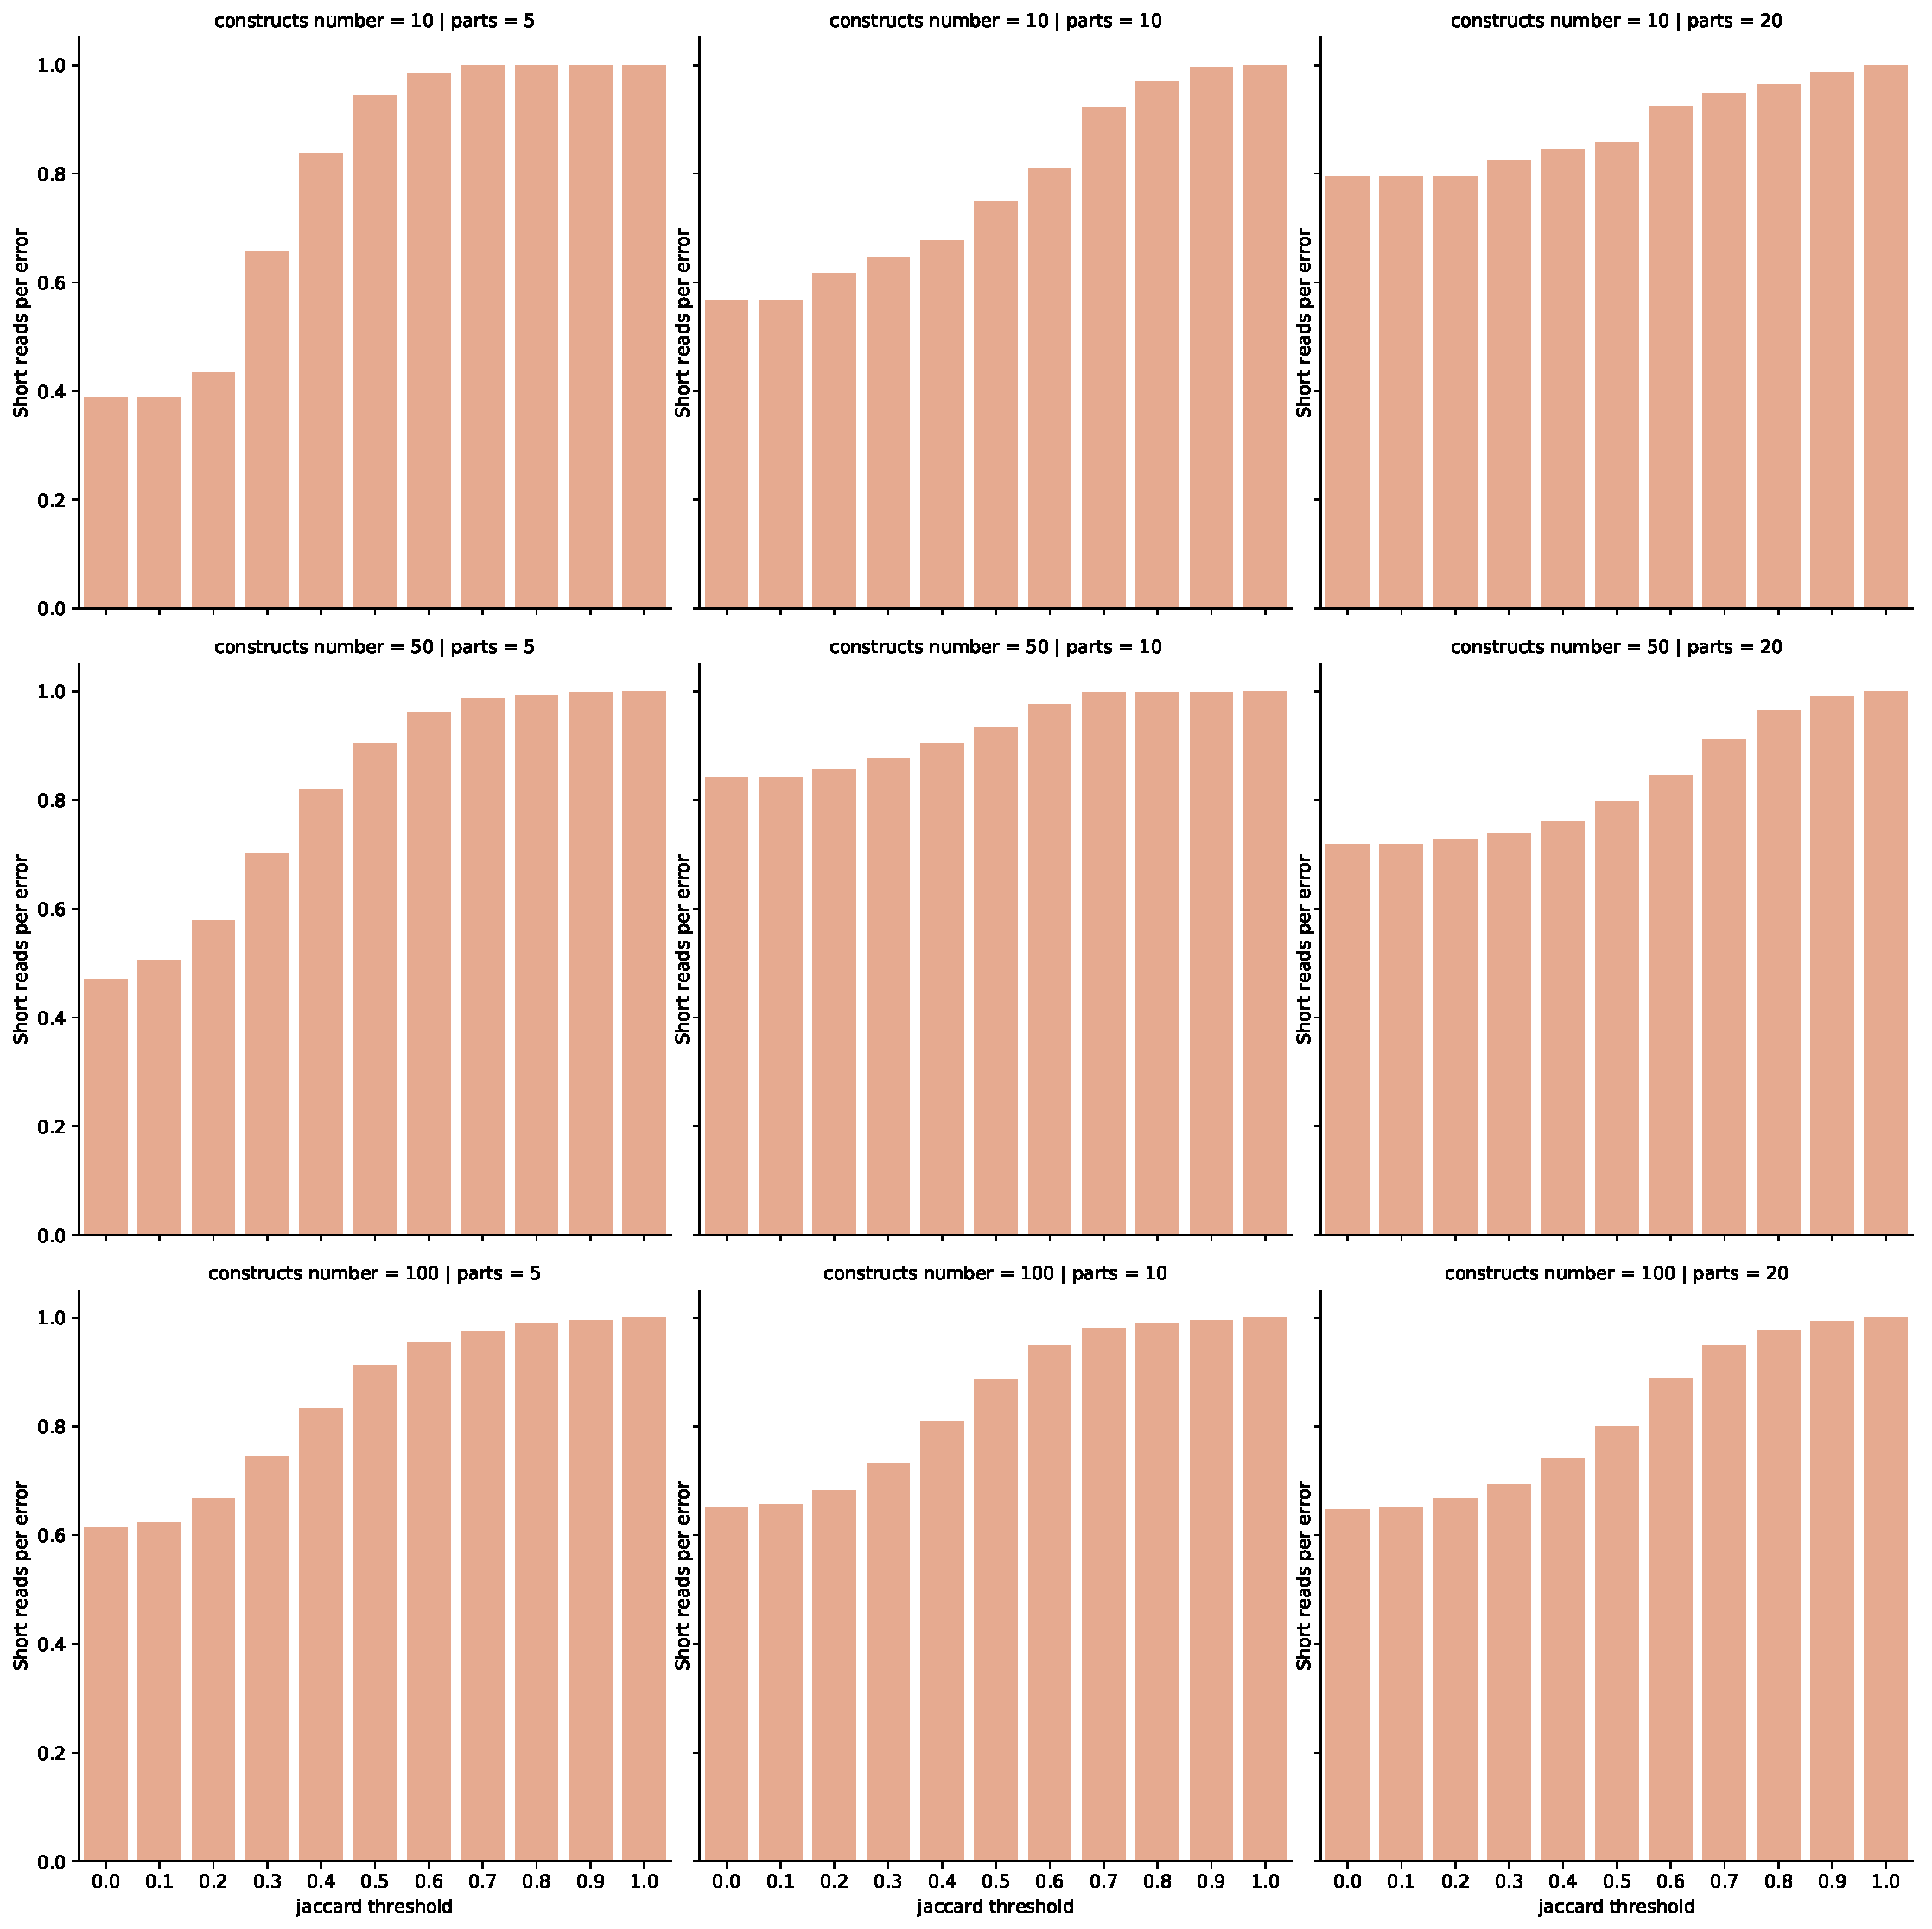
\includegraphics[width=1\textwidth]{../results/images_notebook/v_310/001_short_reads_per_error.pdf}
    \end{center}
    \caption{{\bf Example of a mismatch per error plot taken from run 0. This metric is measured as $read with missing parts/bad matches$ }}
   \label{fig:v_310_shortread_per_error}
\end{figure}

\clearpage

\subsection{V3.1.3 }
This simulation can be executed using the following snakemake config file:
  \begin{lstlisting}[language=Python]
    project: "percentile_5"
    genbank: "yeast_chromosome_xiv.gb"
    run: 1

    generate_testbeds:
        cds_number : 50
        constructs_number: [10,50,100]
        parts : [5,10,20]
        clone_parts_amount : 0.4
        parts_similarity : 0.7

    badreads:
        quantity : "50x"
        error_model: "nanopore"
        qscore_model: "nanopore"
        glitches: "0,0,0"
        junk_reads: 0
        random_reads: 0
        chimeras: 0
        identity: 95,100,4
        start_adapter_seq: ' "" '
        end_adapter_seq: ' "" '

    nanogate:
        error_rate : ["001","010","030"]
        jaccard_thresholds: ["00", "01", "02", "03", "04", 
        "05", "06", "07", "08", "09", "10"]
\end{lstlisting}


\begin{figure}[ht]
    \begin{center}
    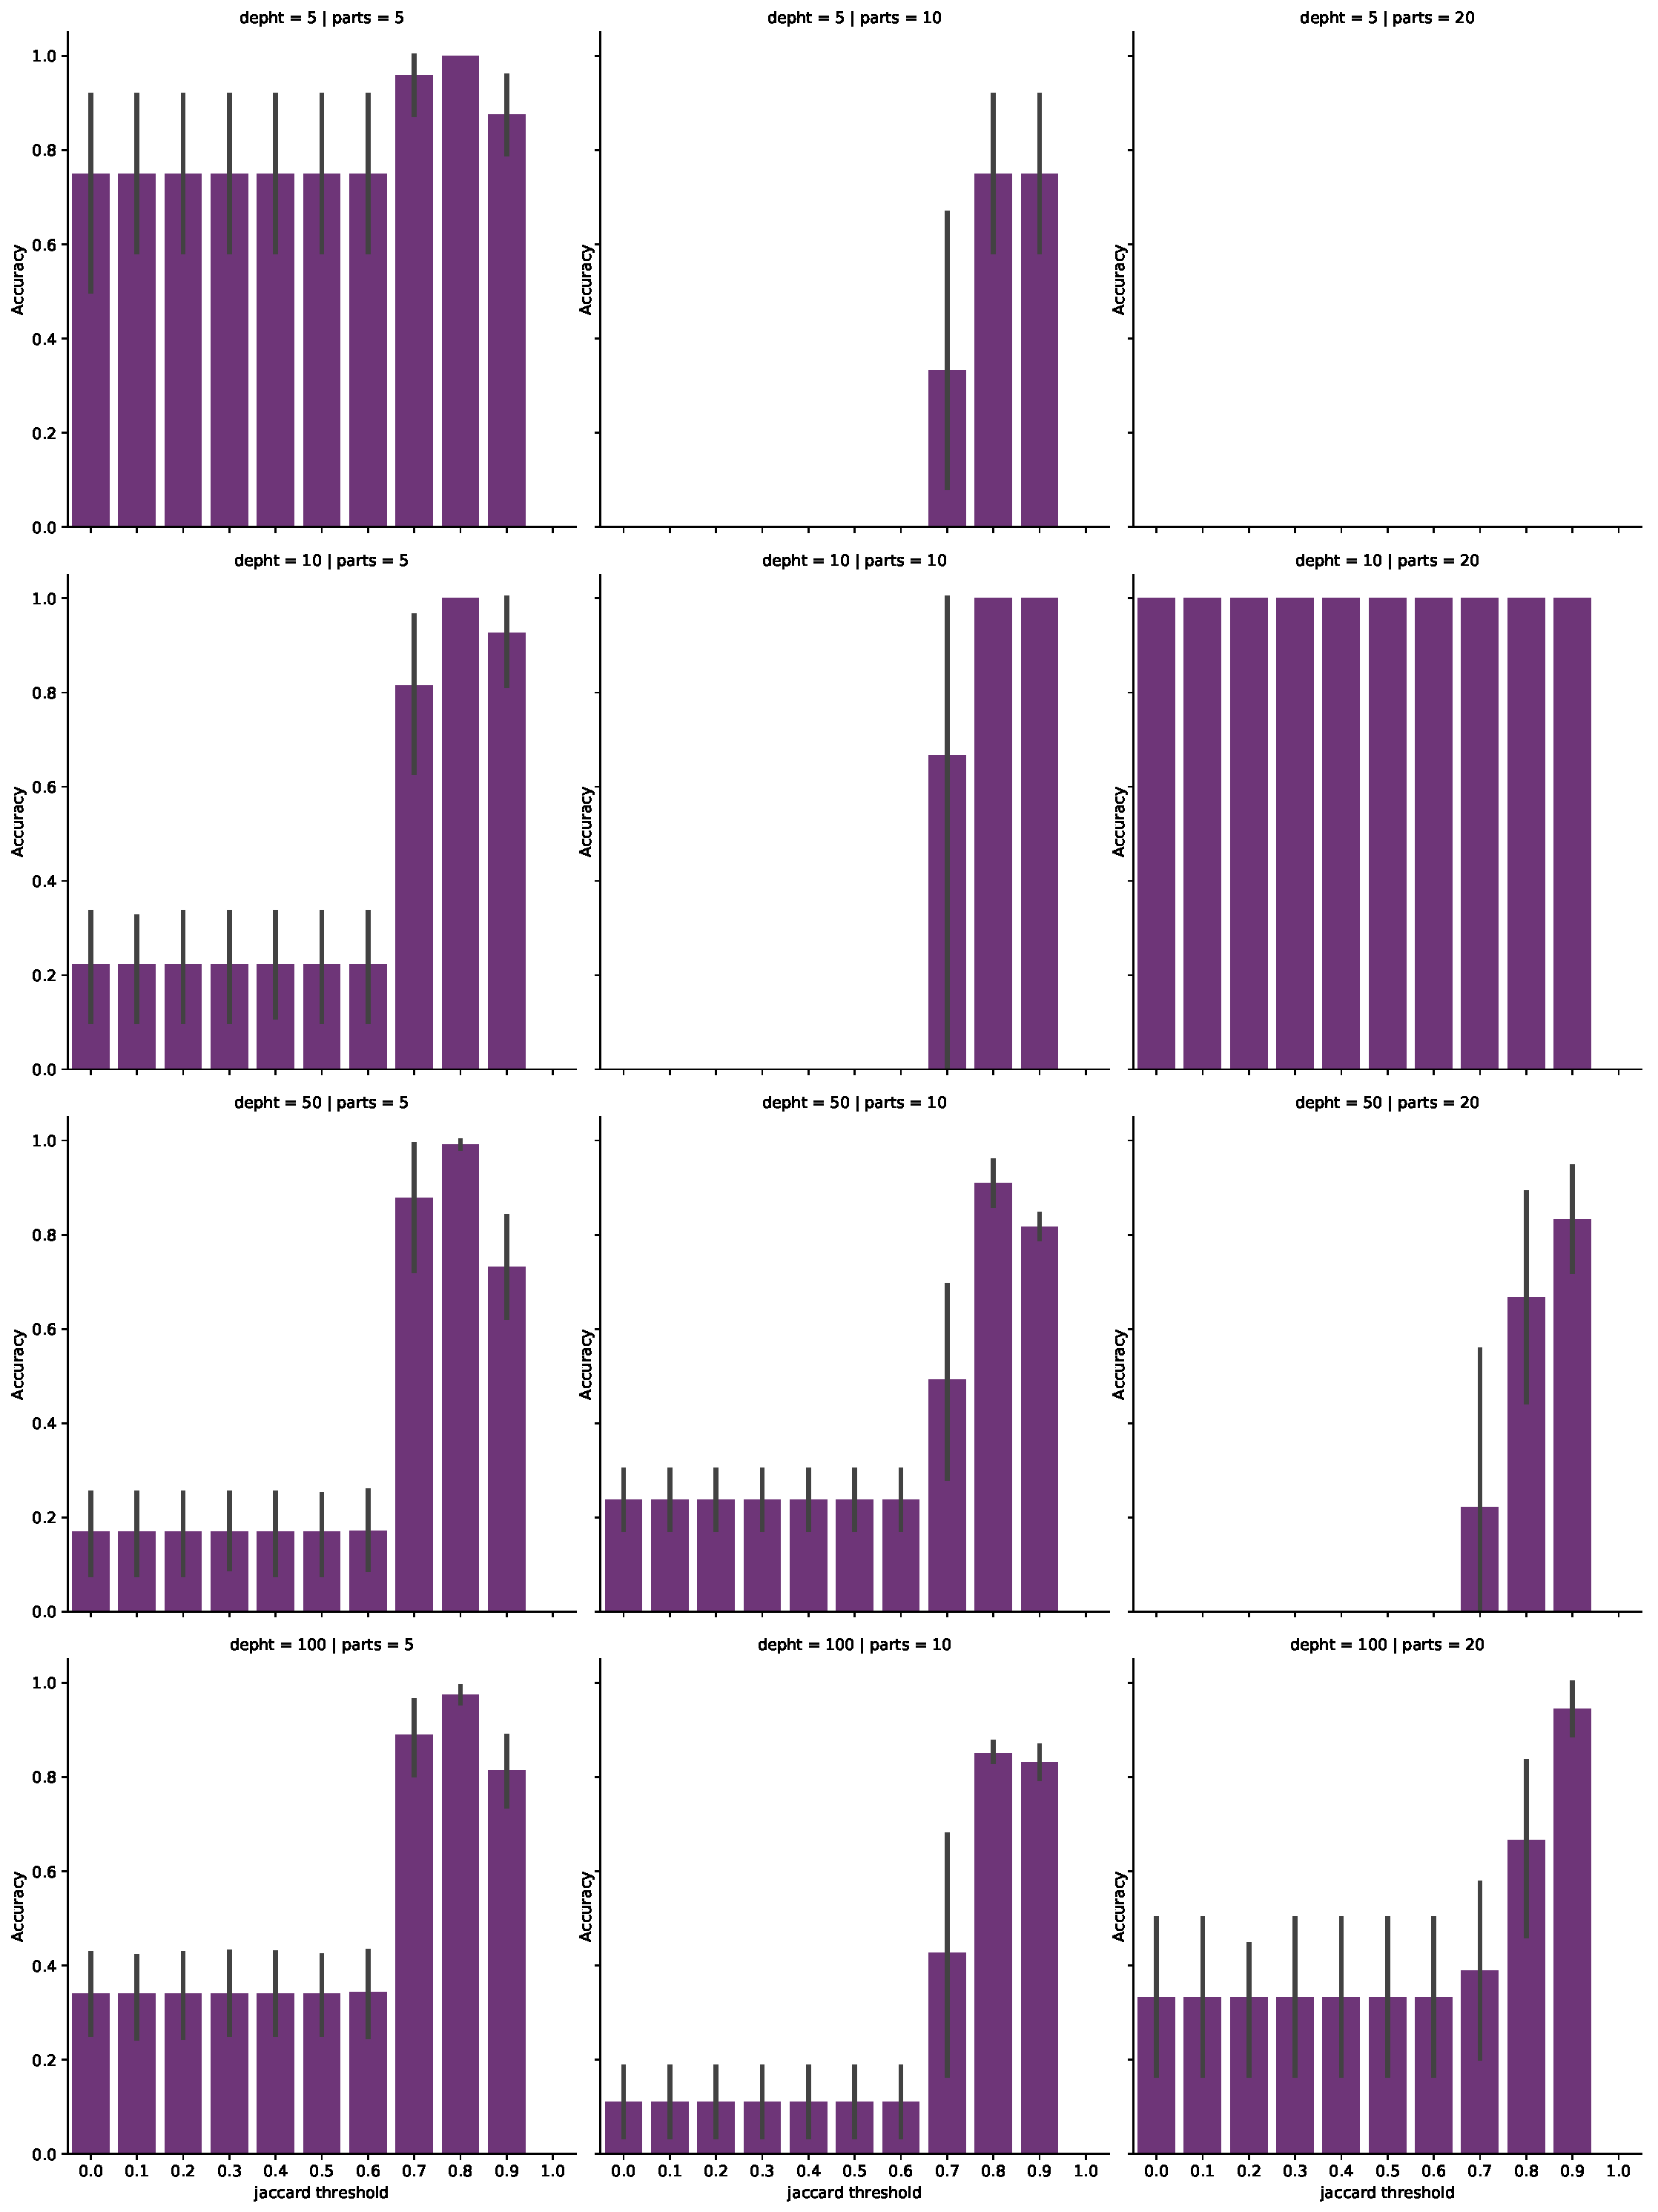
\includegraphics[width=1\textwidth]{../results/images_notebook/v_312/good_reads_true_positves.pdf}
    \end{center}
    \caption{{\bf True positives analysed only on good reads }}
   \label{fig:v_312_good_reads_true_positves}
\end{figure}

\begin{figure}[ht]
    \begin{center}
    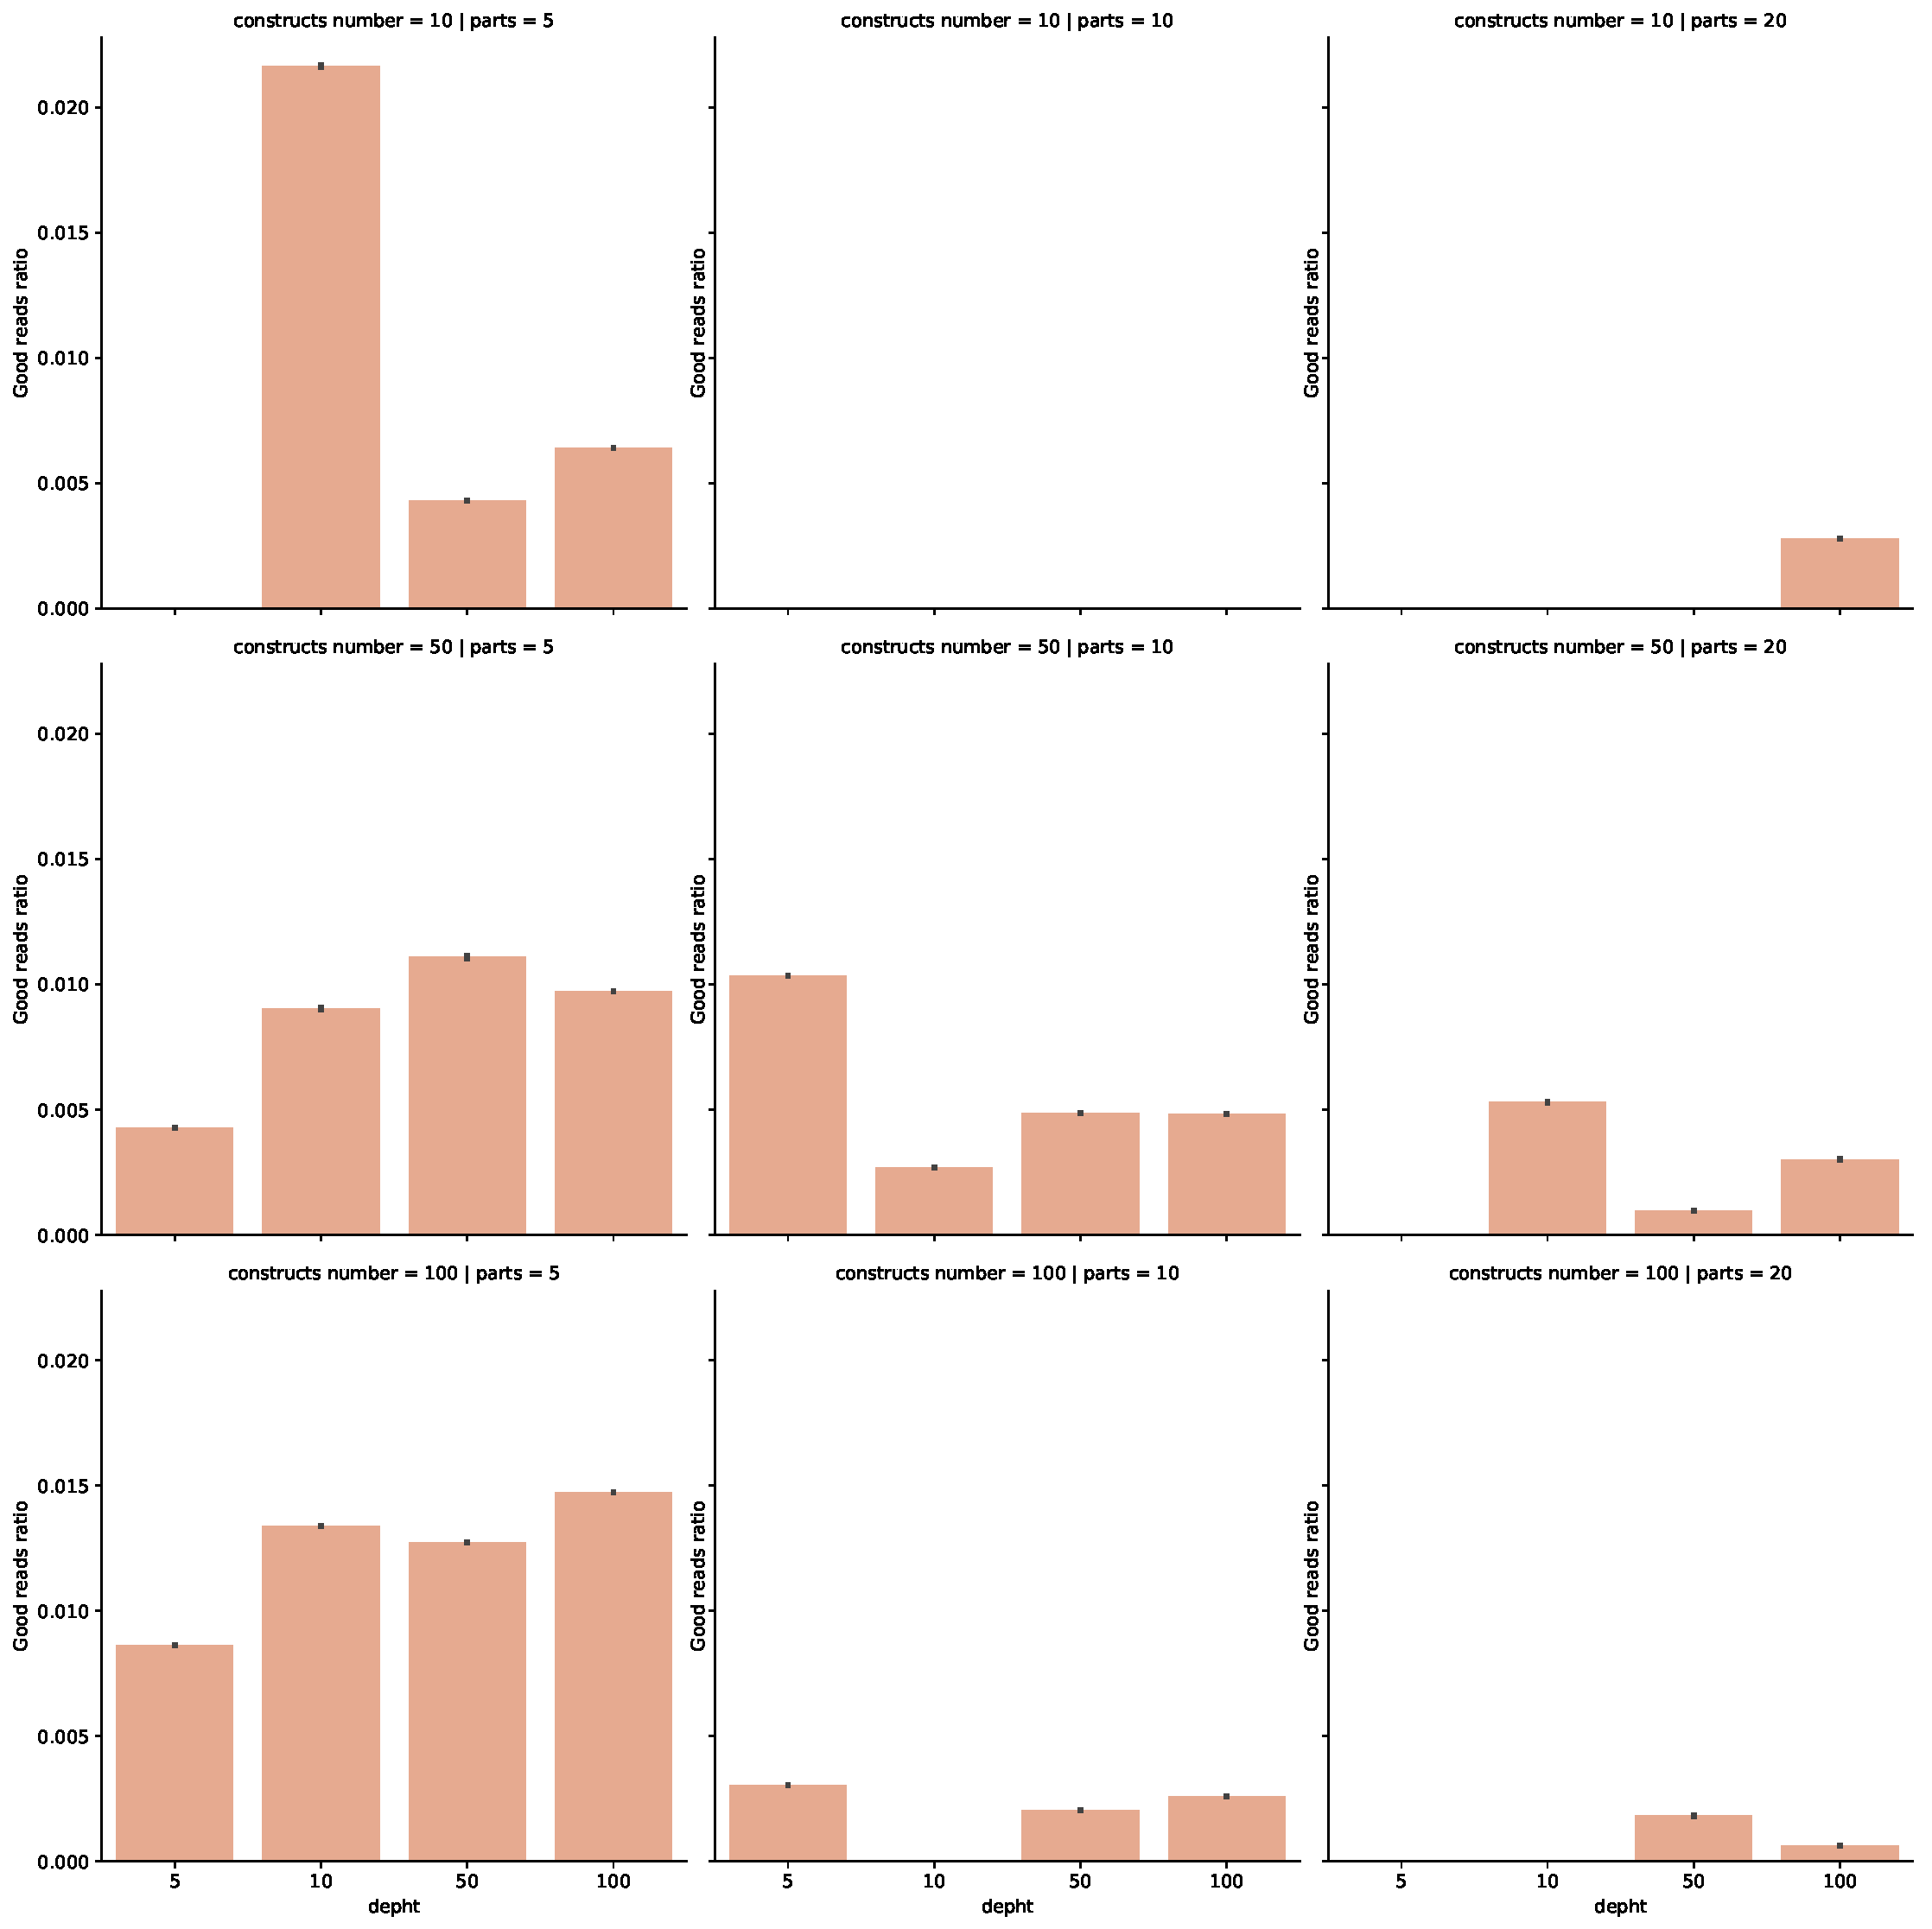
\includegraphics[width=1\textwidth]{../results/images_notebook/v_312/good_reads_ratio.pdf}
    \end{center}
    \caption{{\bf Good reeads/all reads }}
   \label{fig:v_312_good_reads_ratio}
\end{figure}

\begin{figure}[ht]
    \begin{center}
    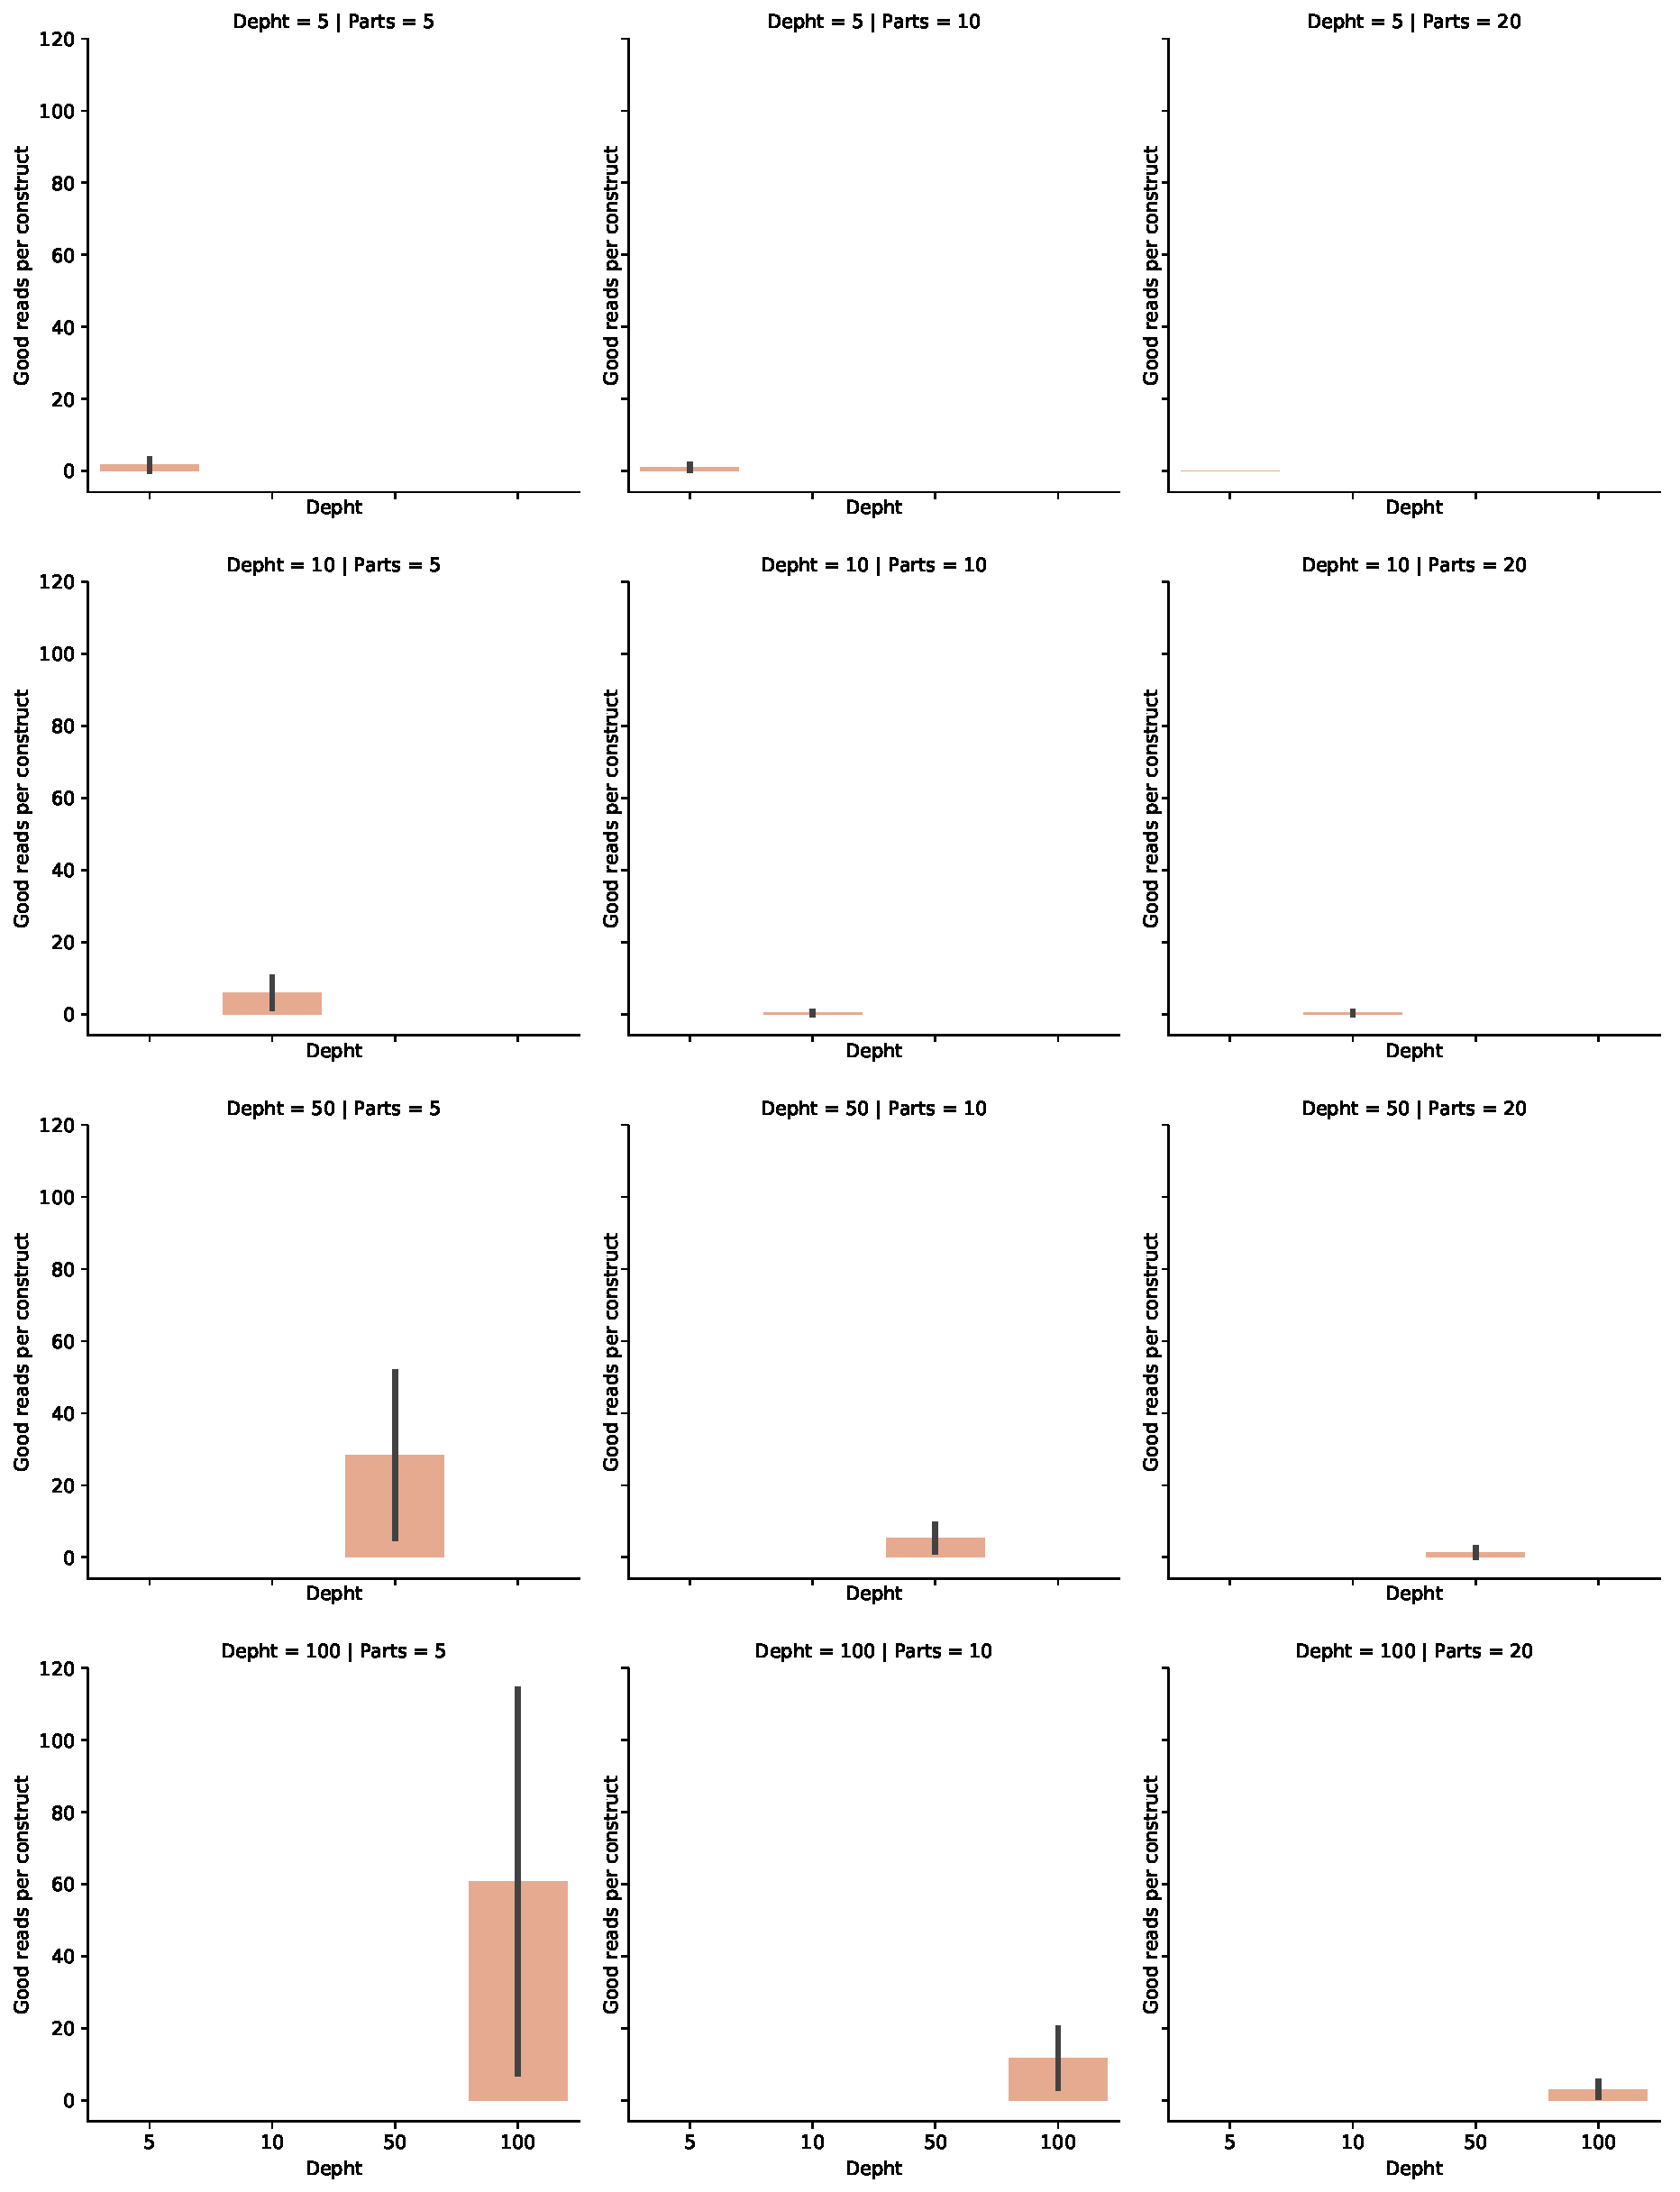
\includegraphics[width=1\textwidth]{../results/images_notebook/v_312/good_reads_plot.pdf}
    \end{center}
    \caption{{\bf Good reeads by depth }}
   \label{fig:v_312_good_reads_plot.r}
\end{figure}

\begin{figure}[ht]
    \begin{center}
    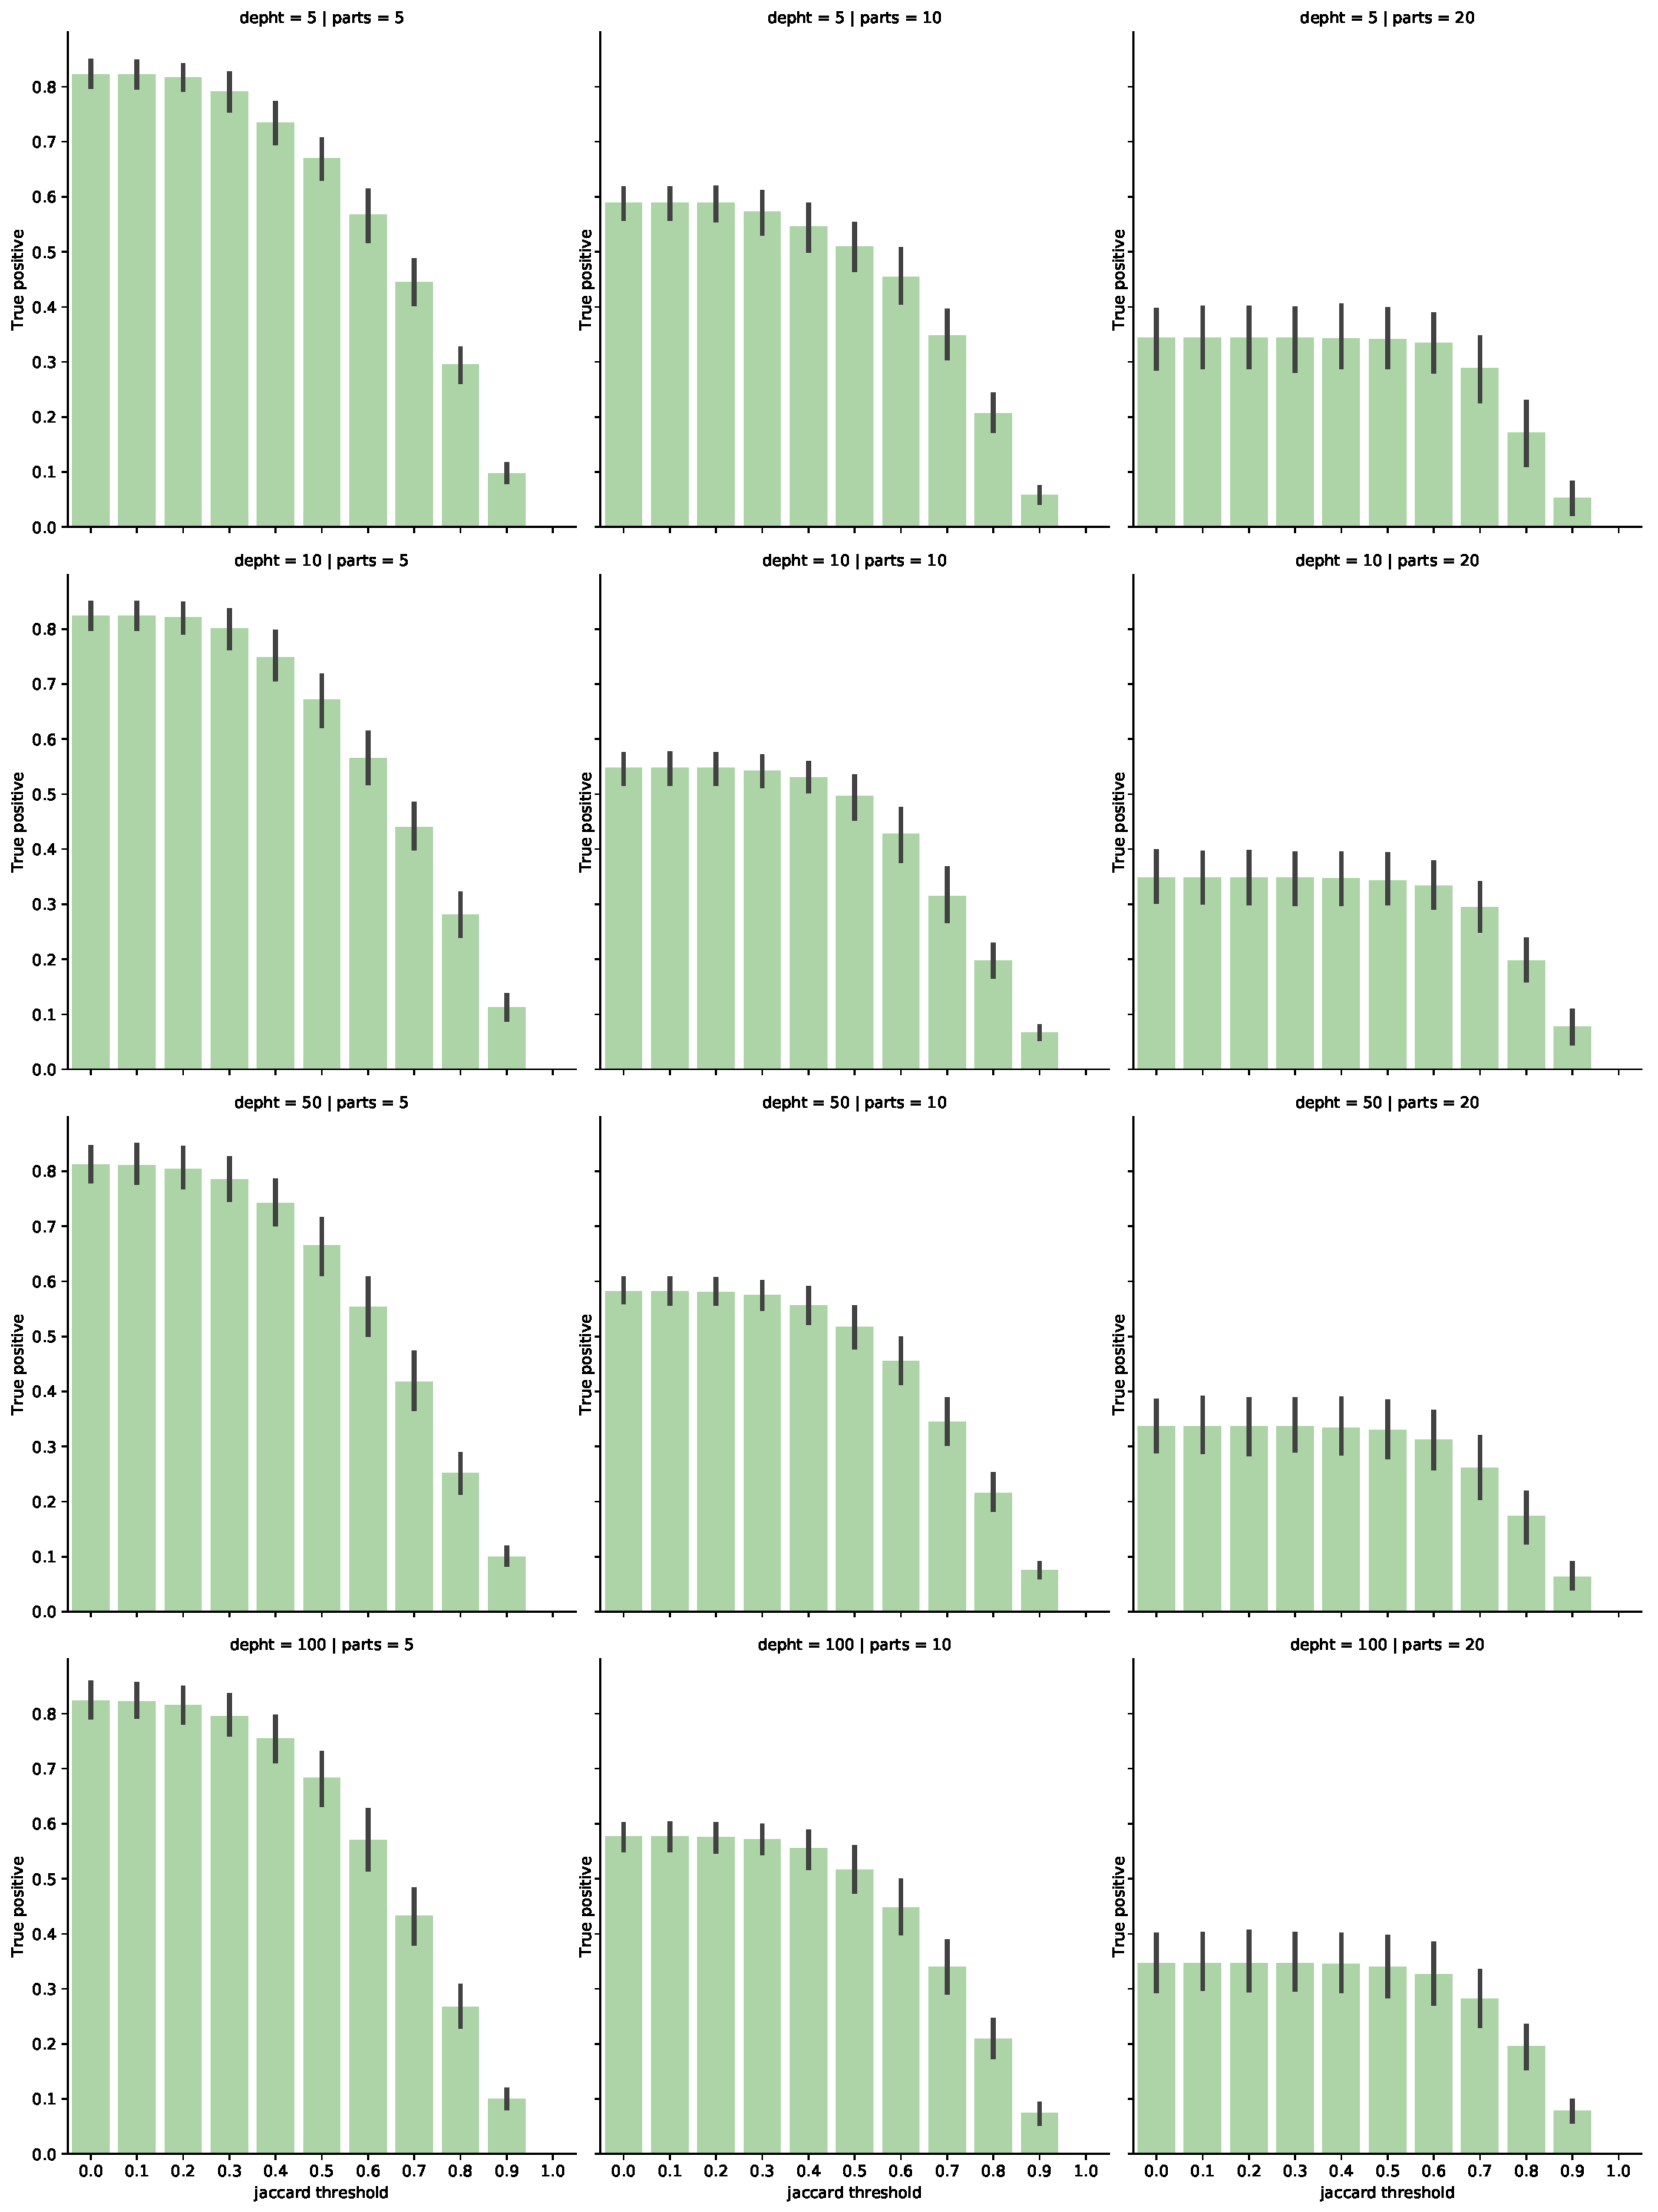
\includegraphics[width=1\textwidth]{../results/images_notebook/v_312/true_positive.pdf}
    \end{center}
    \caption{{\bf true postives by depht }}
   \label{fig:v_312_true_positive.}
\end{figure}

\begin{figure}[ht]
    \begin{center}
    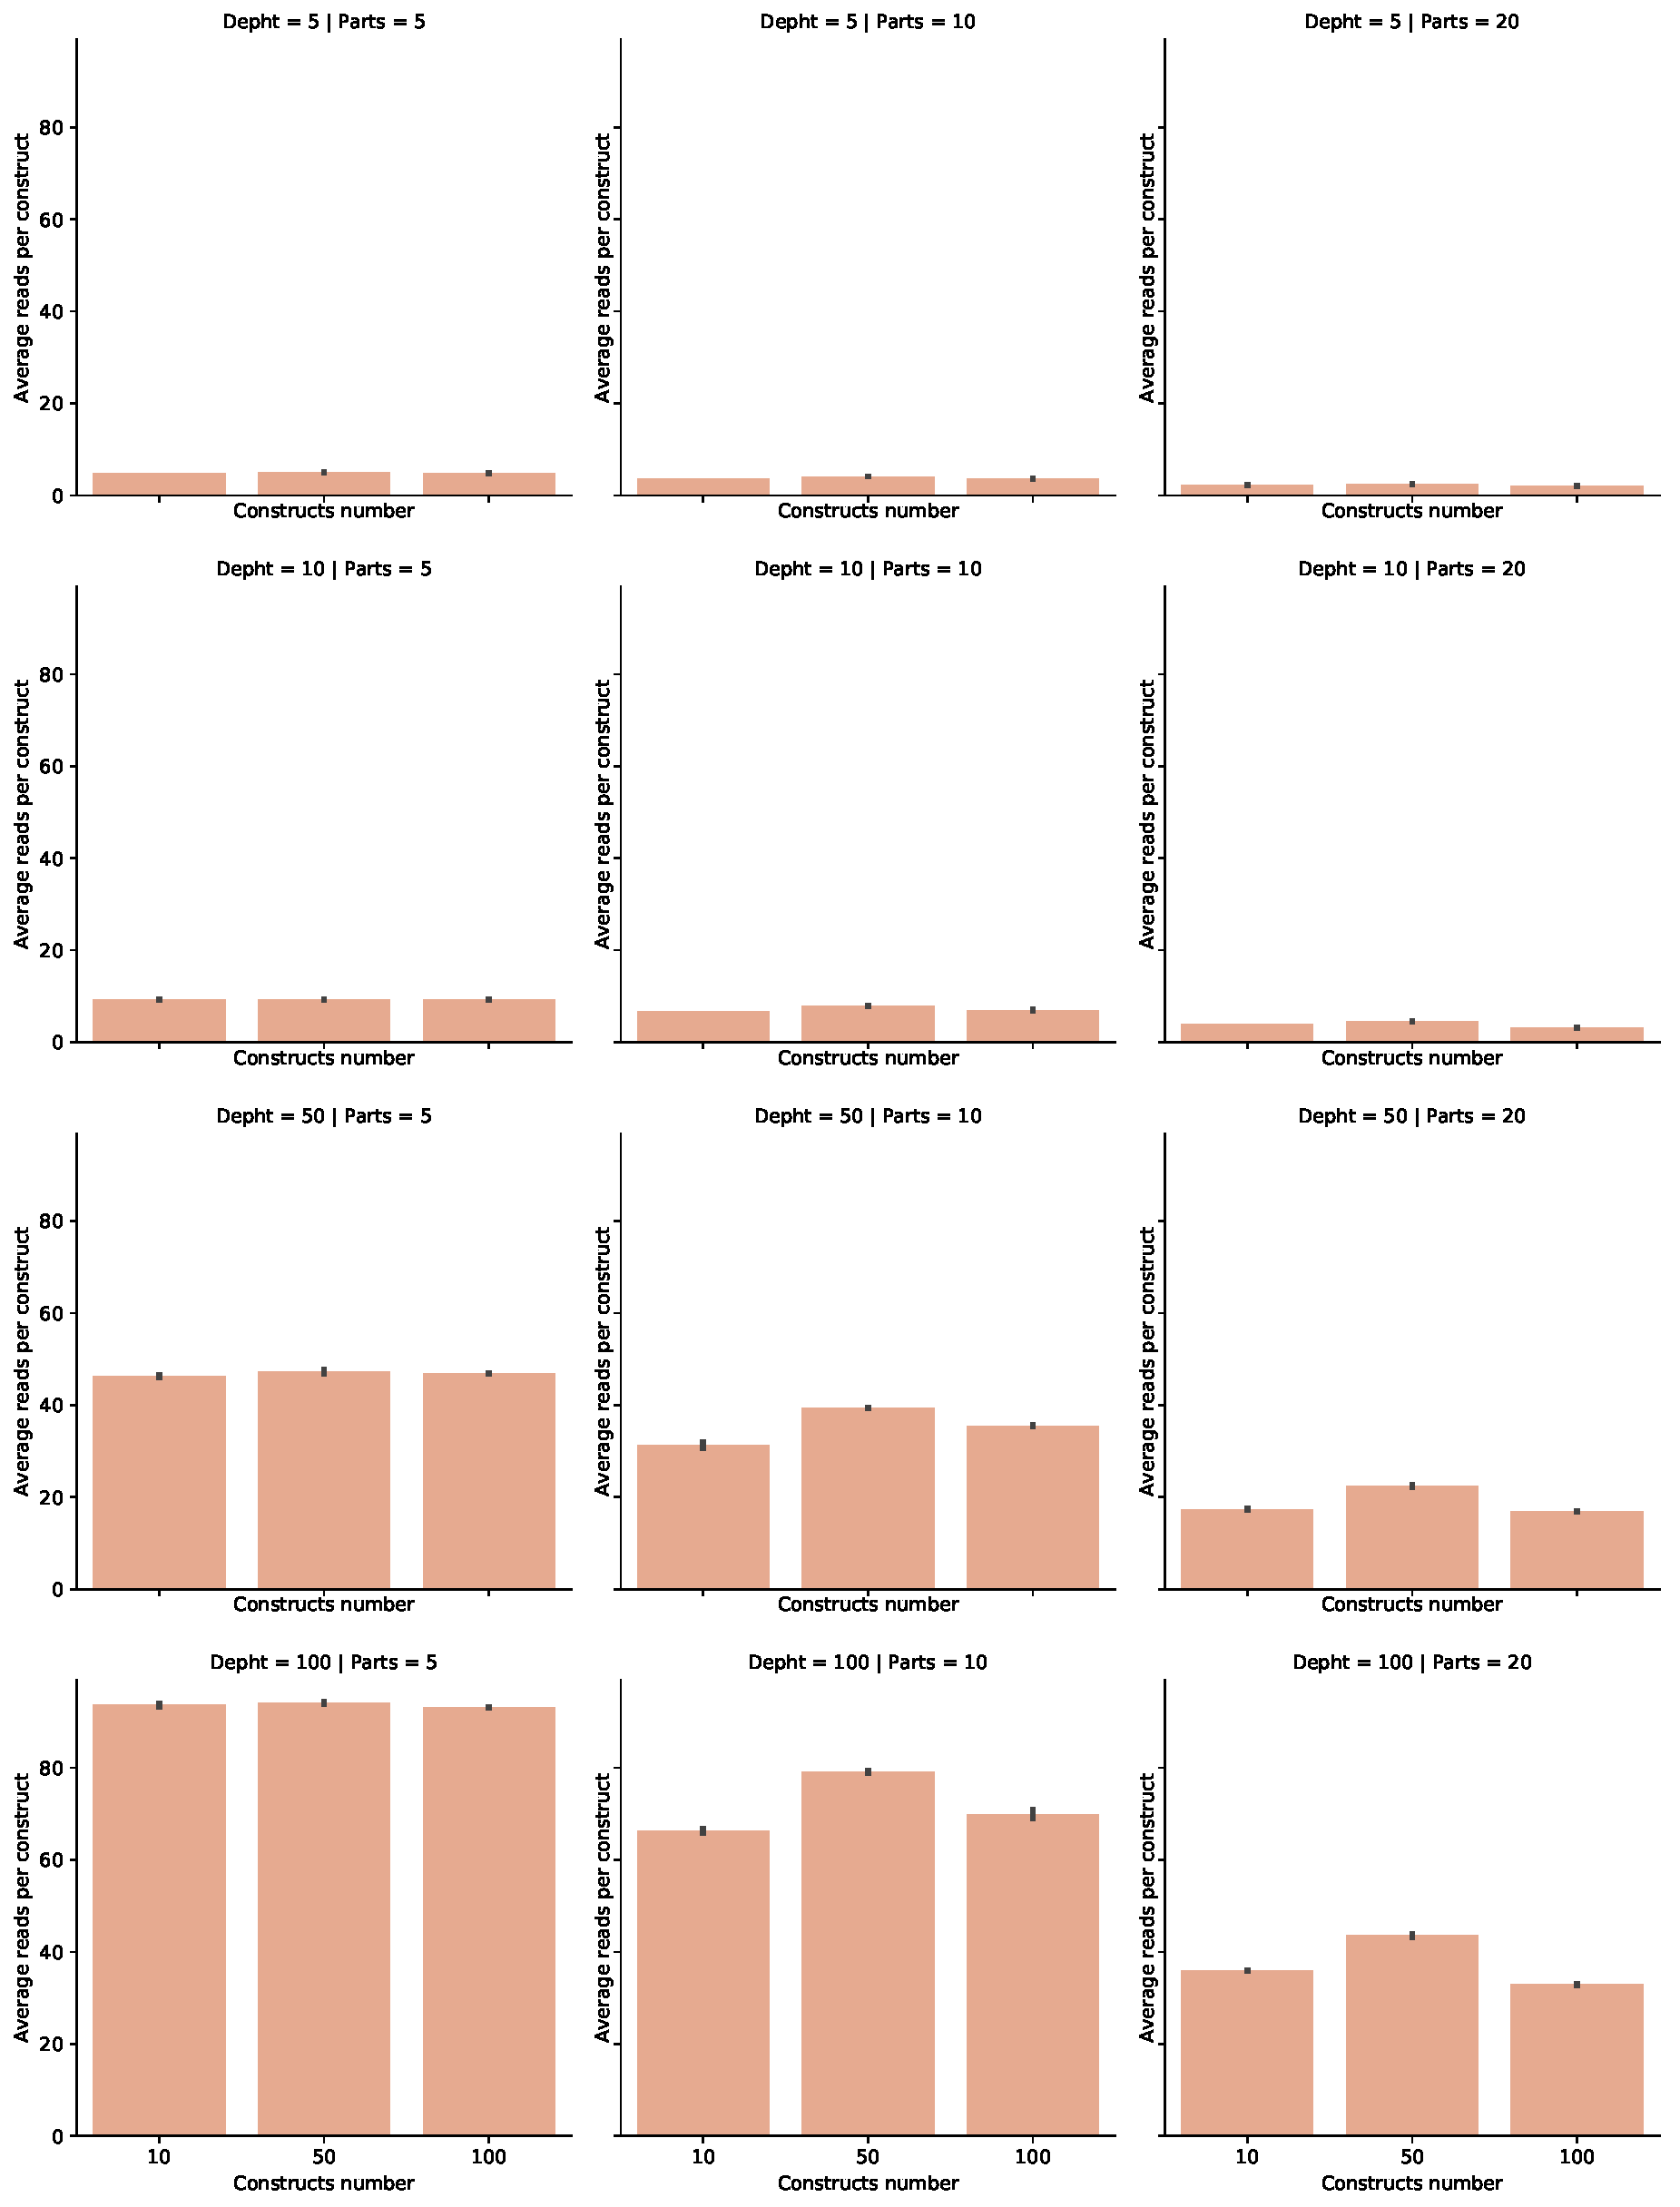
\includegraphics[width=1\textwidth]{../results/images_notebook/v_312/average_reads.pdf}
    \end{center}
    \caption{{\bf average reads analysed per construct }}
   \label{fig:v_312_average_reads}
\end{figure}

\clearpage

\subsection{V3.2.1 }
\subsubsection{Good read filter}
Accuracy is defined as:
$Good reads true postives/ good reads$
\textbf{Good reads} = the number of reads with a length $\geq$ of $99\%$ of the orignal construct
\textbf{Good reads true positives} = \textbf{Good reads} matching with the expected parts in the orignal construct




\begin{figure}[ht]
    \begin{center}
    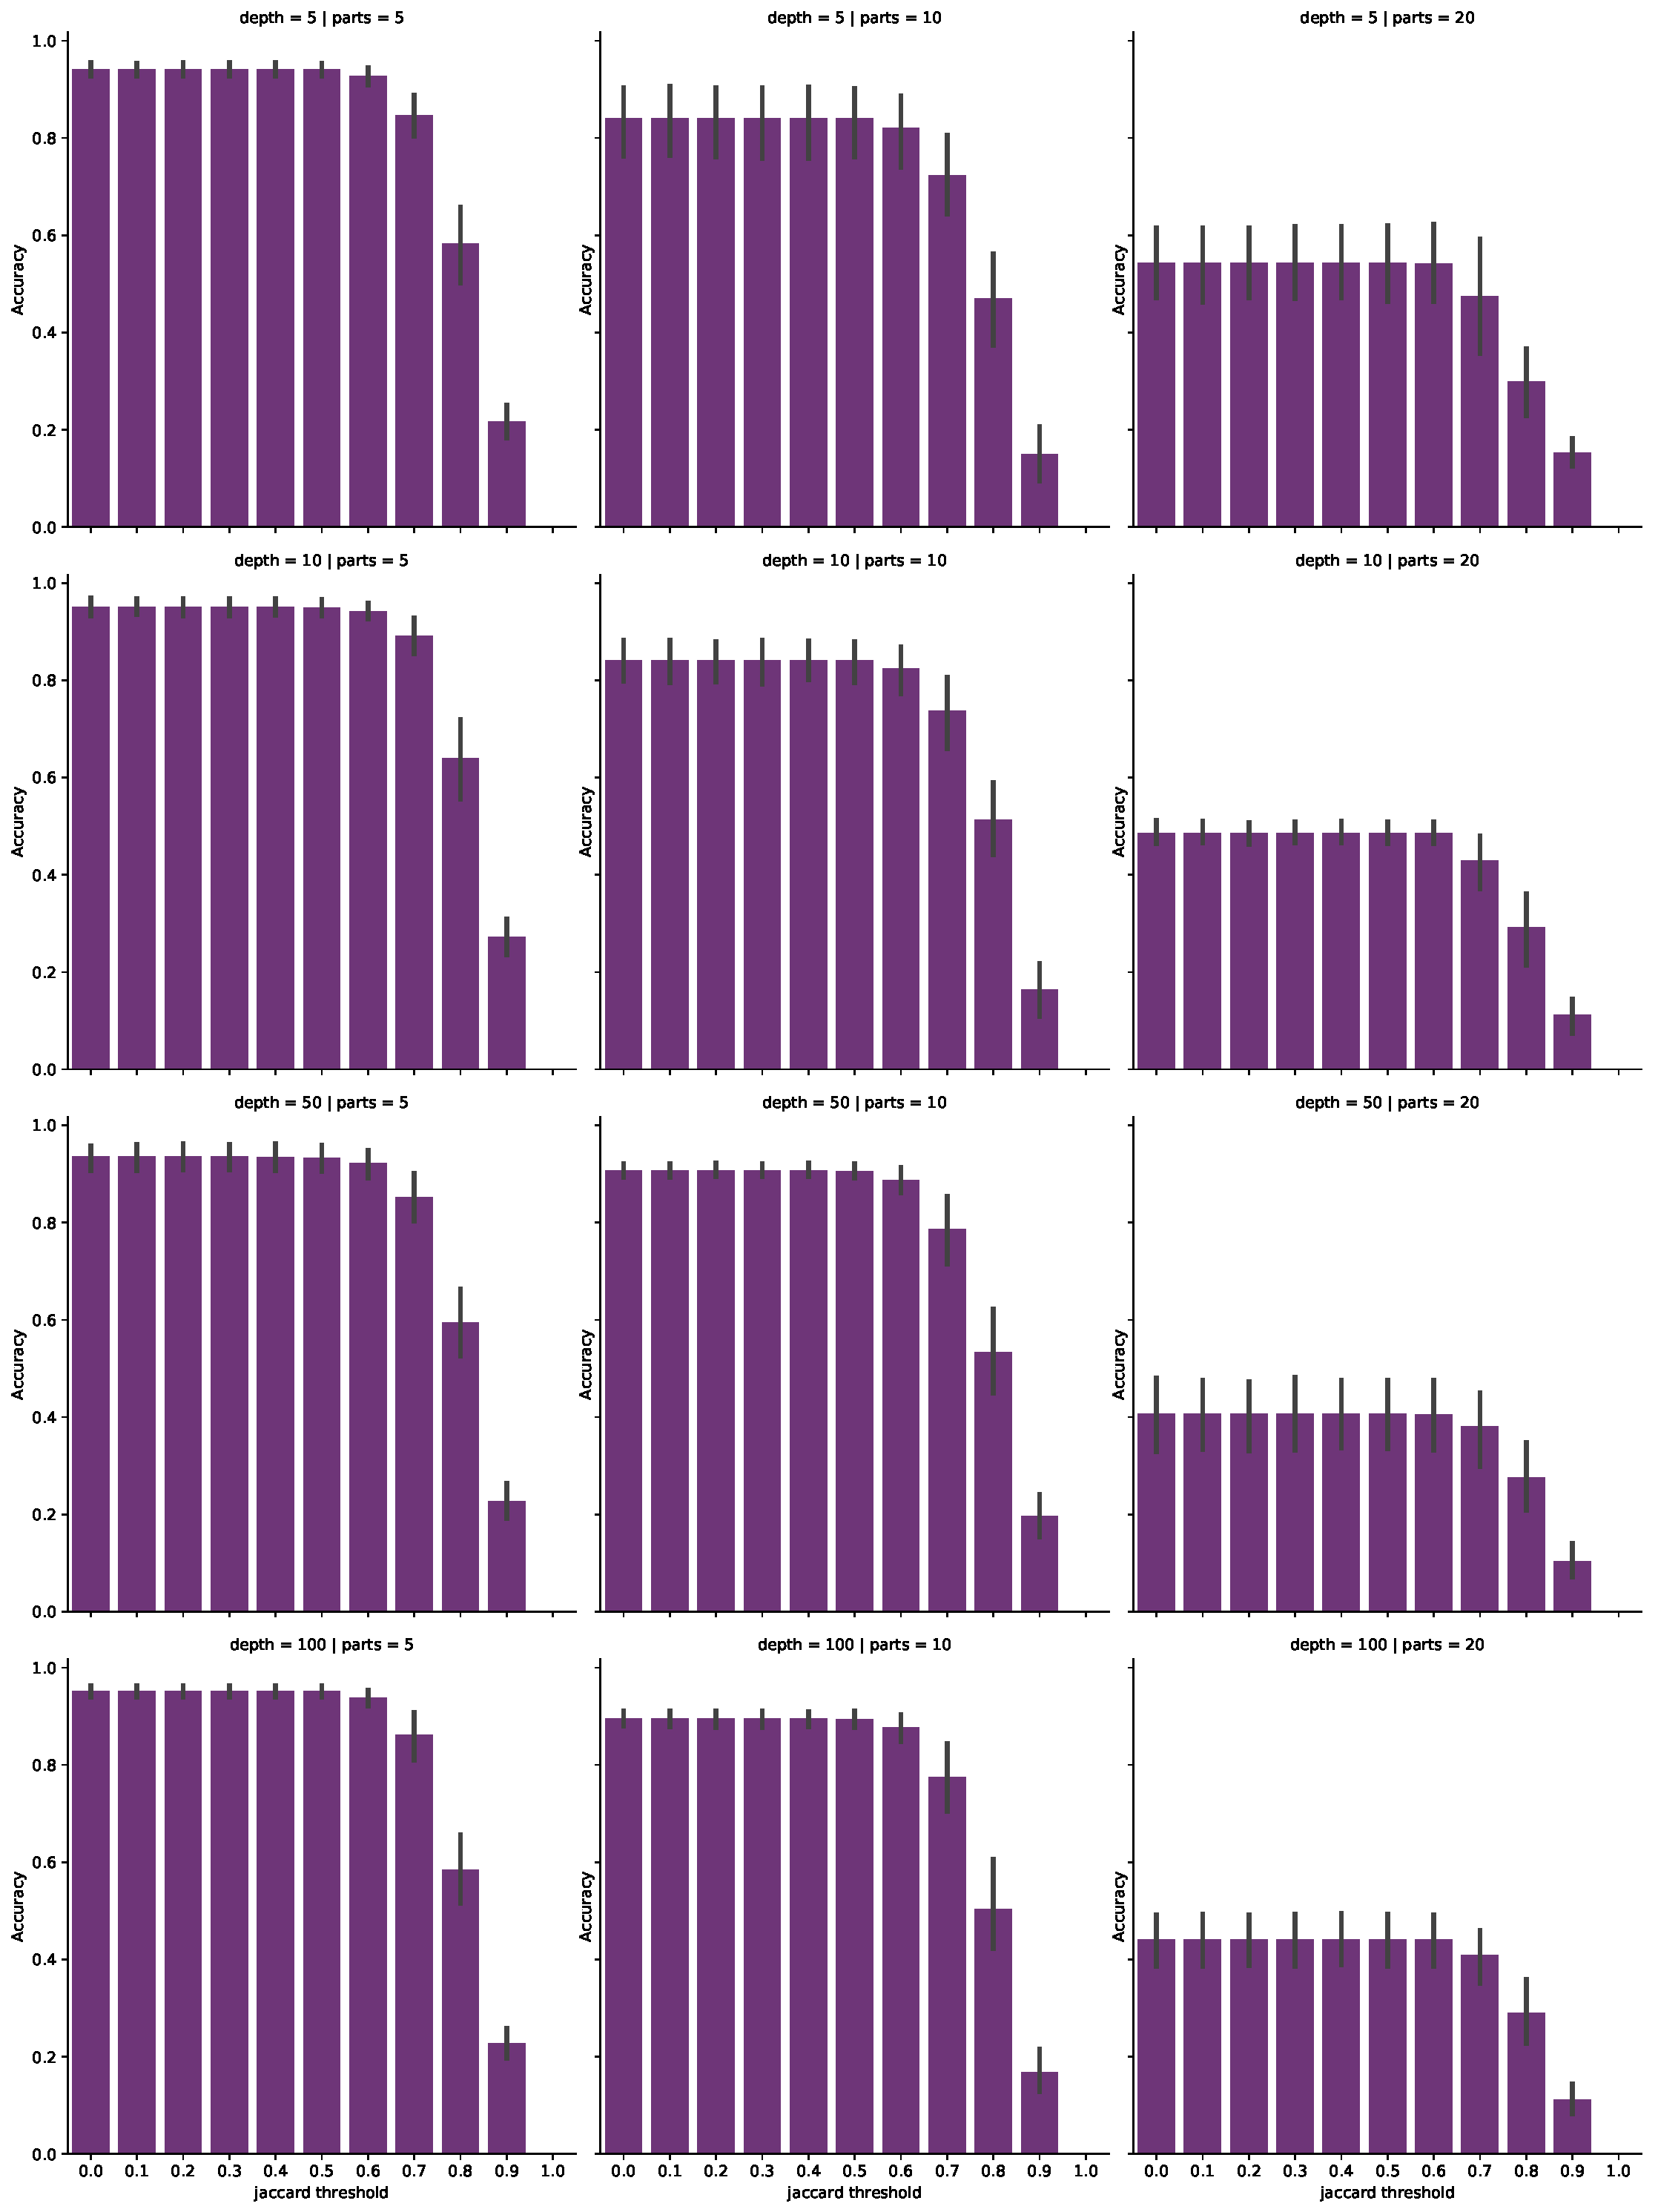
\includegraphics[width=1\textwidth]{../results/images_notebook/v_322/99_good_reads_true_positves.pdf}
    \end{center}
    \caption{{\bf accuracy $99\%$}}
   \label{fig:v_320_accuracy_99}
\end{figure}


\begin{figure}[ht]
    \begin{center}
    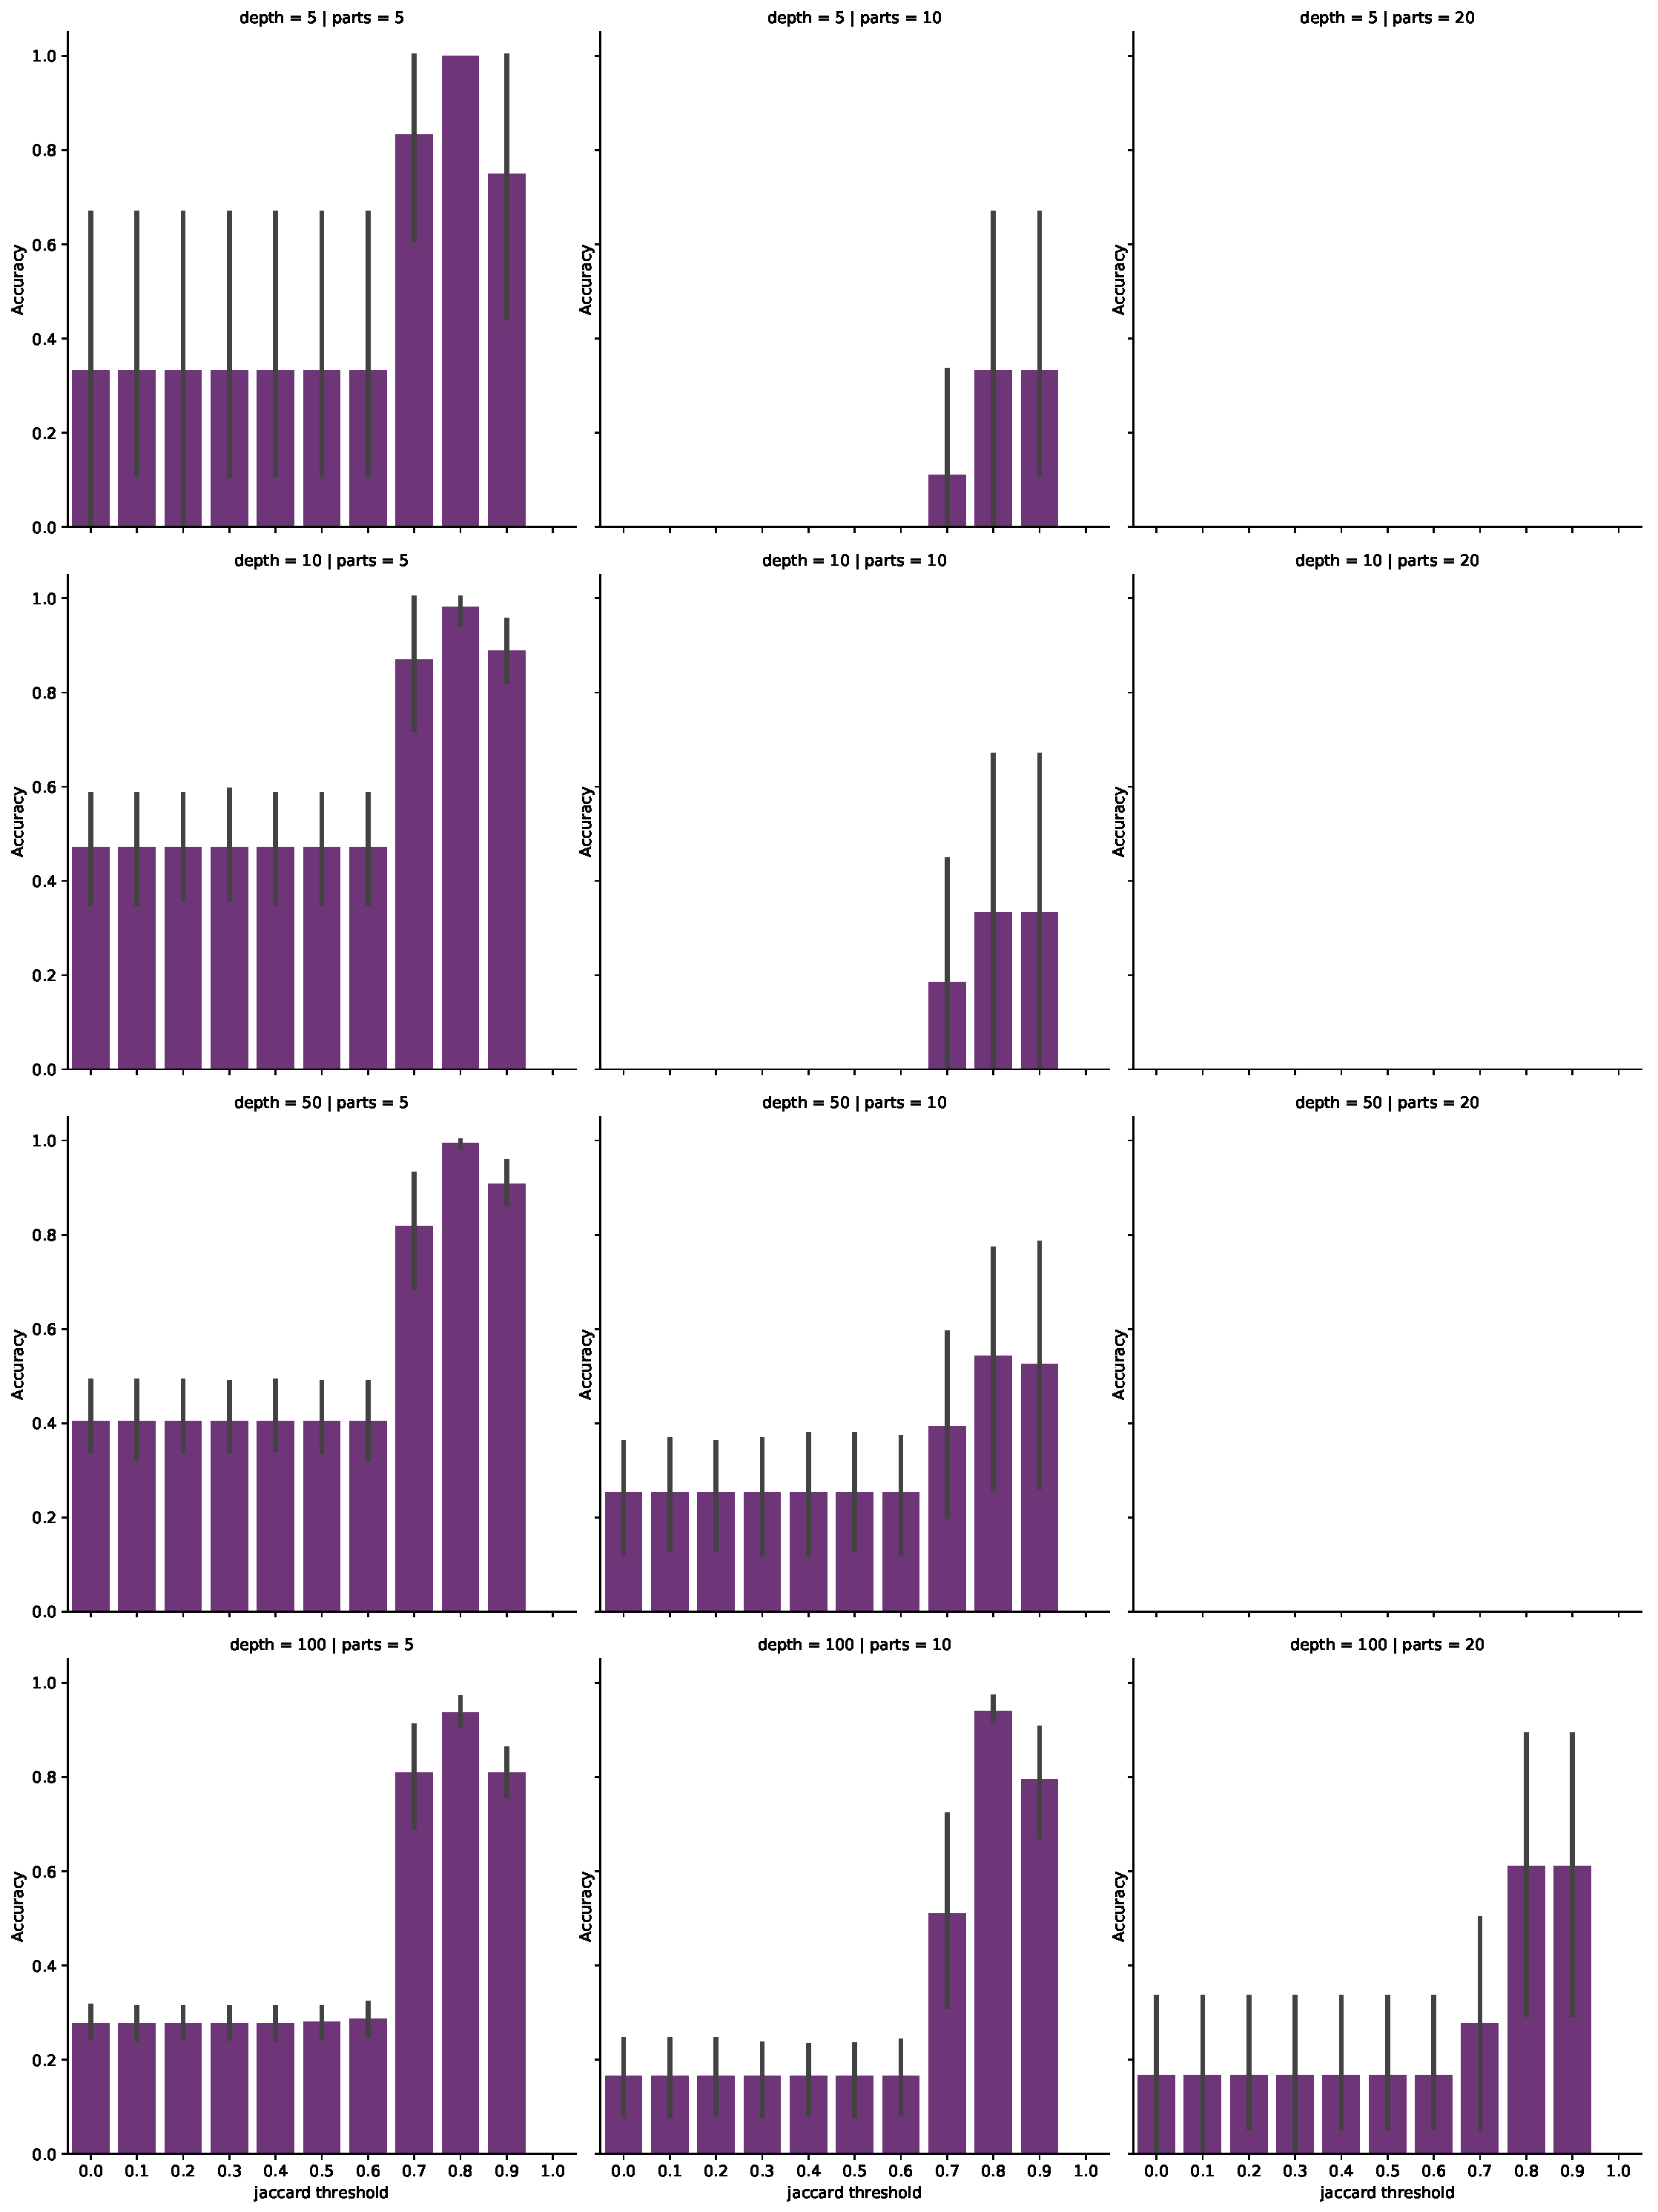
\includegraphics[width=1\textwidth]{../results/images_notebook/v_322/100_good_reads_true_positves.pdf}
    \end{center}
    \caption{{\bf accuracy $100\%$}}
   \label{fig:v_322_accuracy_100}
\end{figure}

\subsubsection{Good reads amount}
Evaluating amount of good reads
\textbf{Good reads} = the number of reads with a length $\geq$ of $99\%$ of the orignal construct

\begin{figure}[ht]
    \begin{center}
    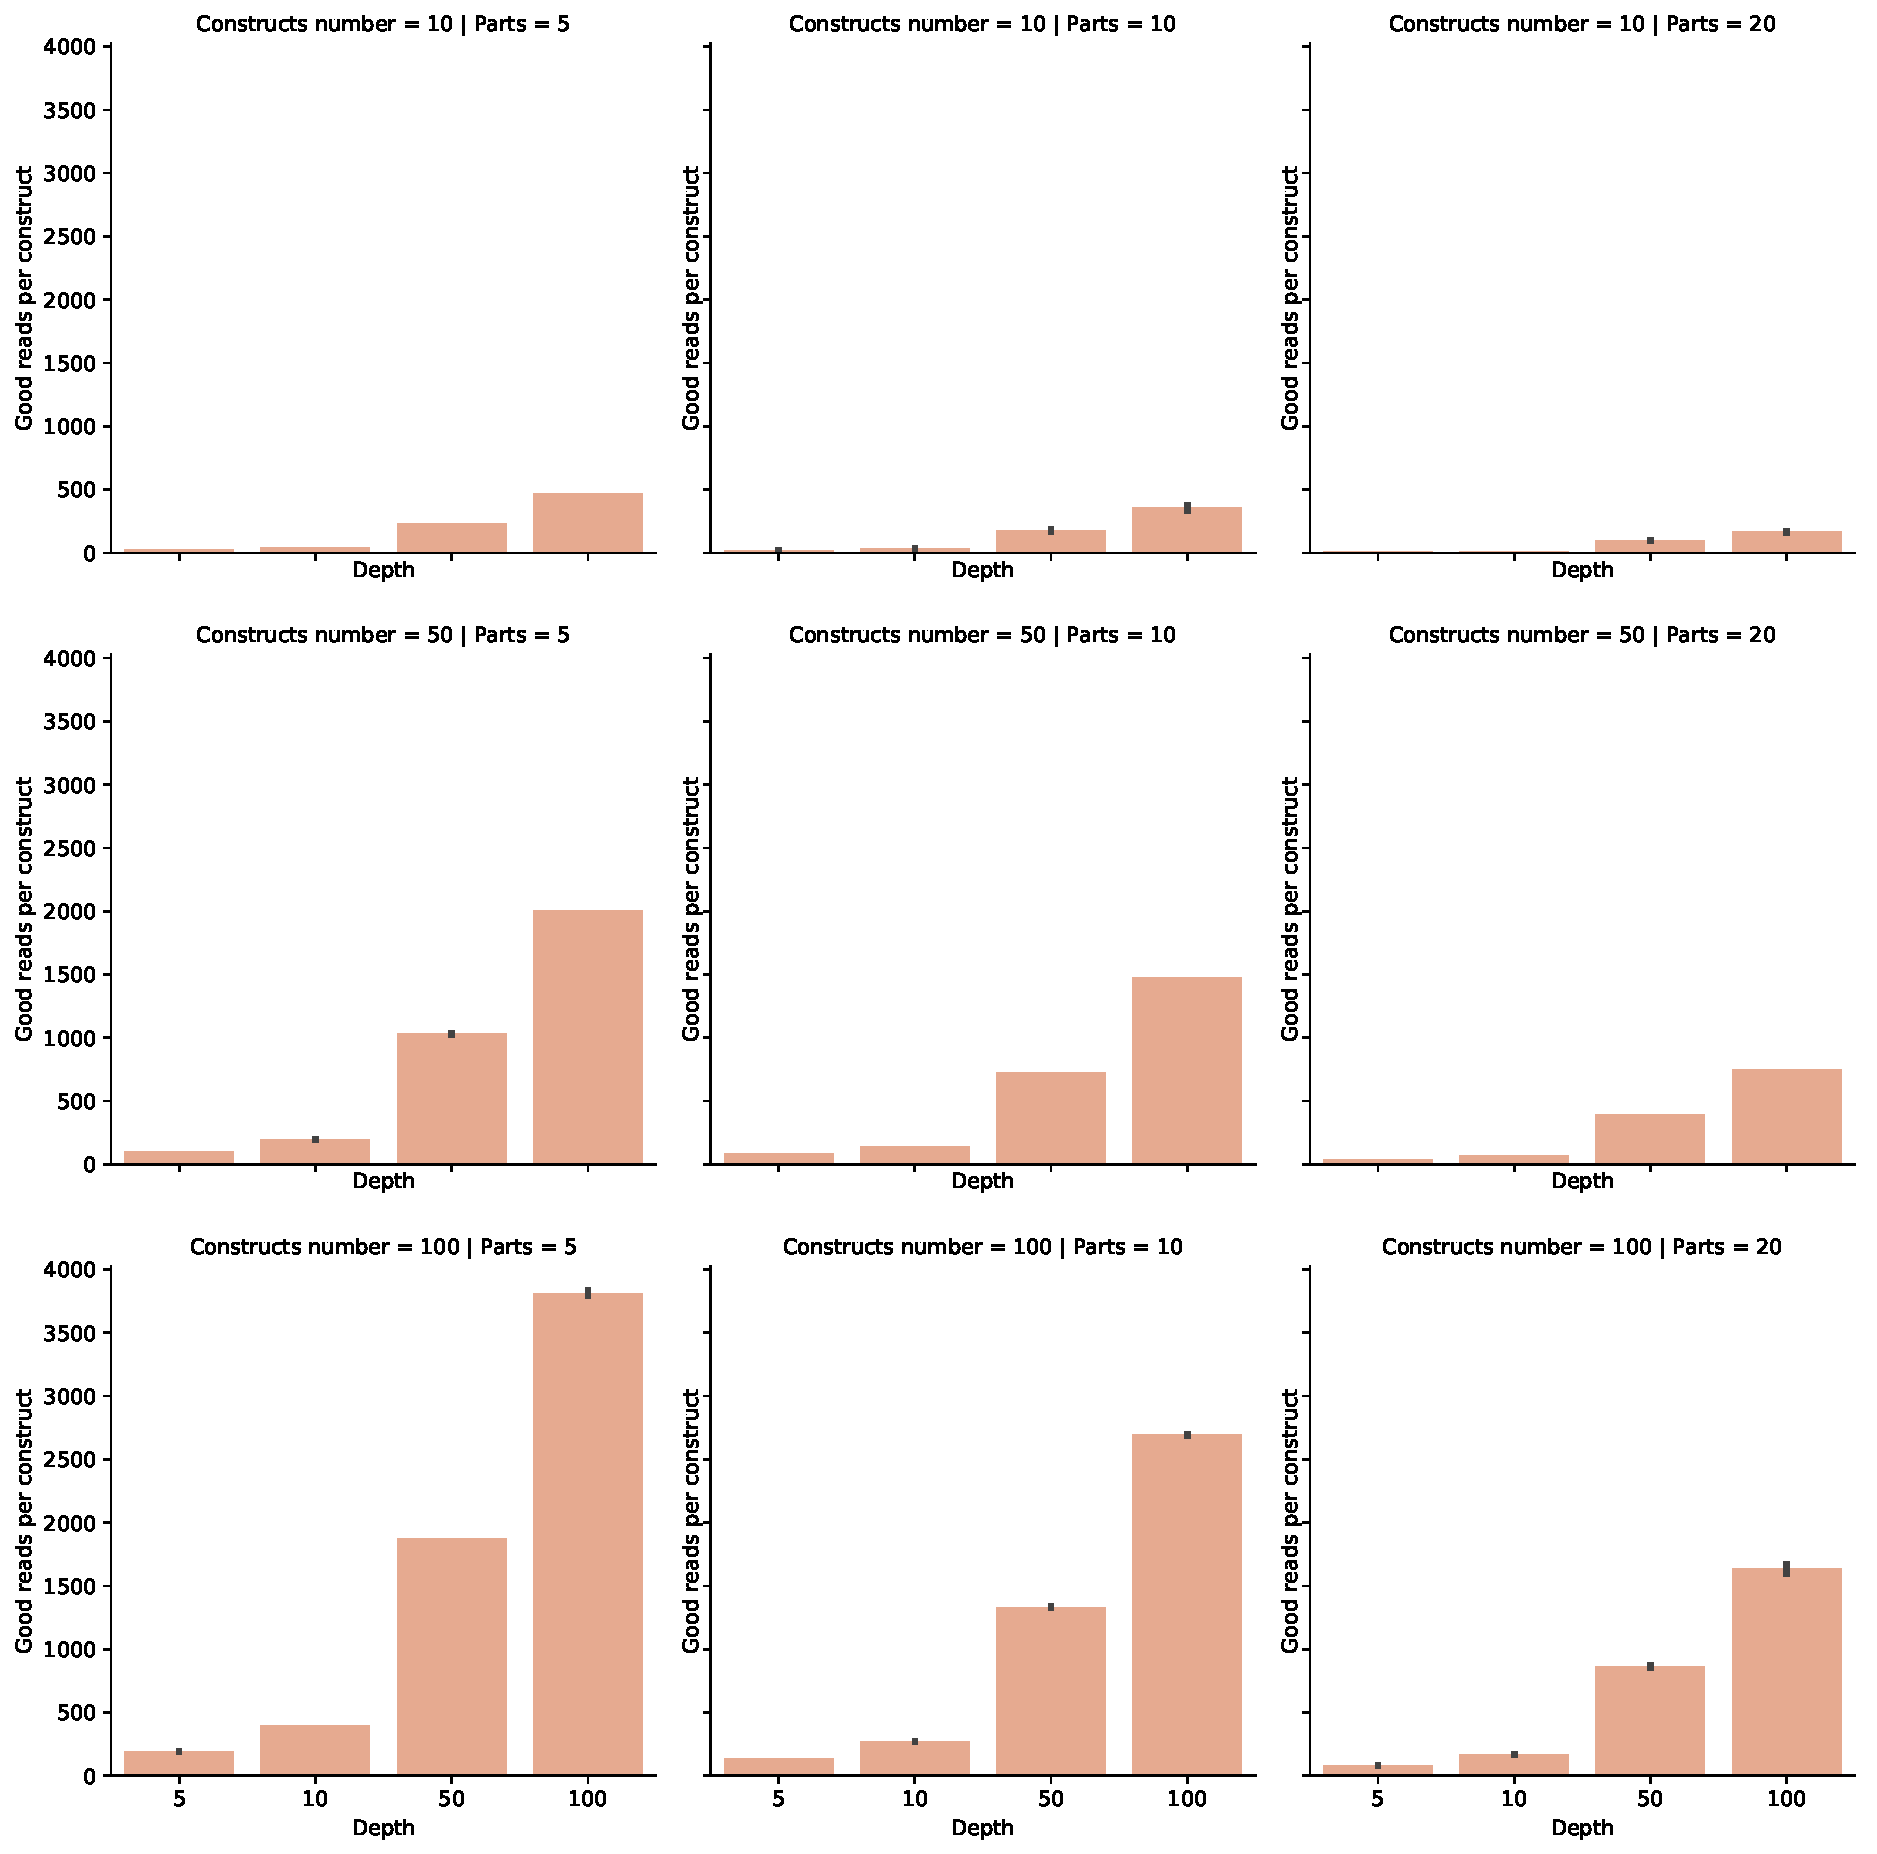
\includegraphics[width=1\textwidth]{../results/images_notebook/v_322/99_good_reads_plot.pdf}
    \end{center}
    \caption{{\bf good reads $99\%$}}
   \label{fig:v_322_good_reads_99}
\end{figure}

\begin{figure}[ht]
    \begin{center}
    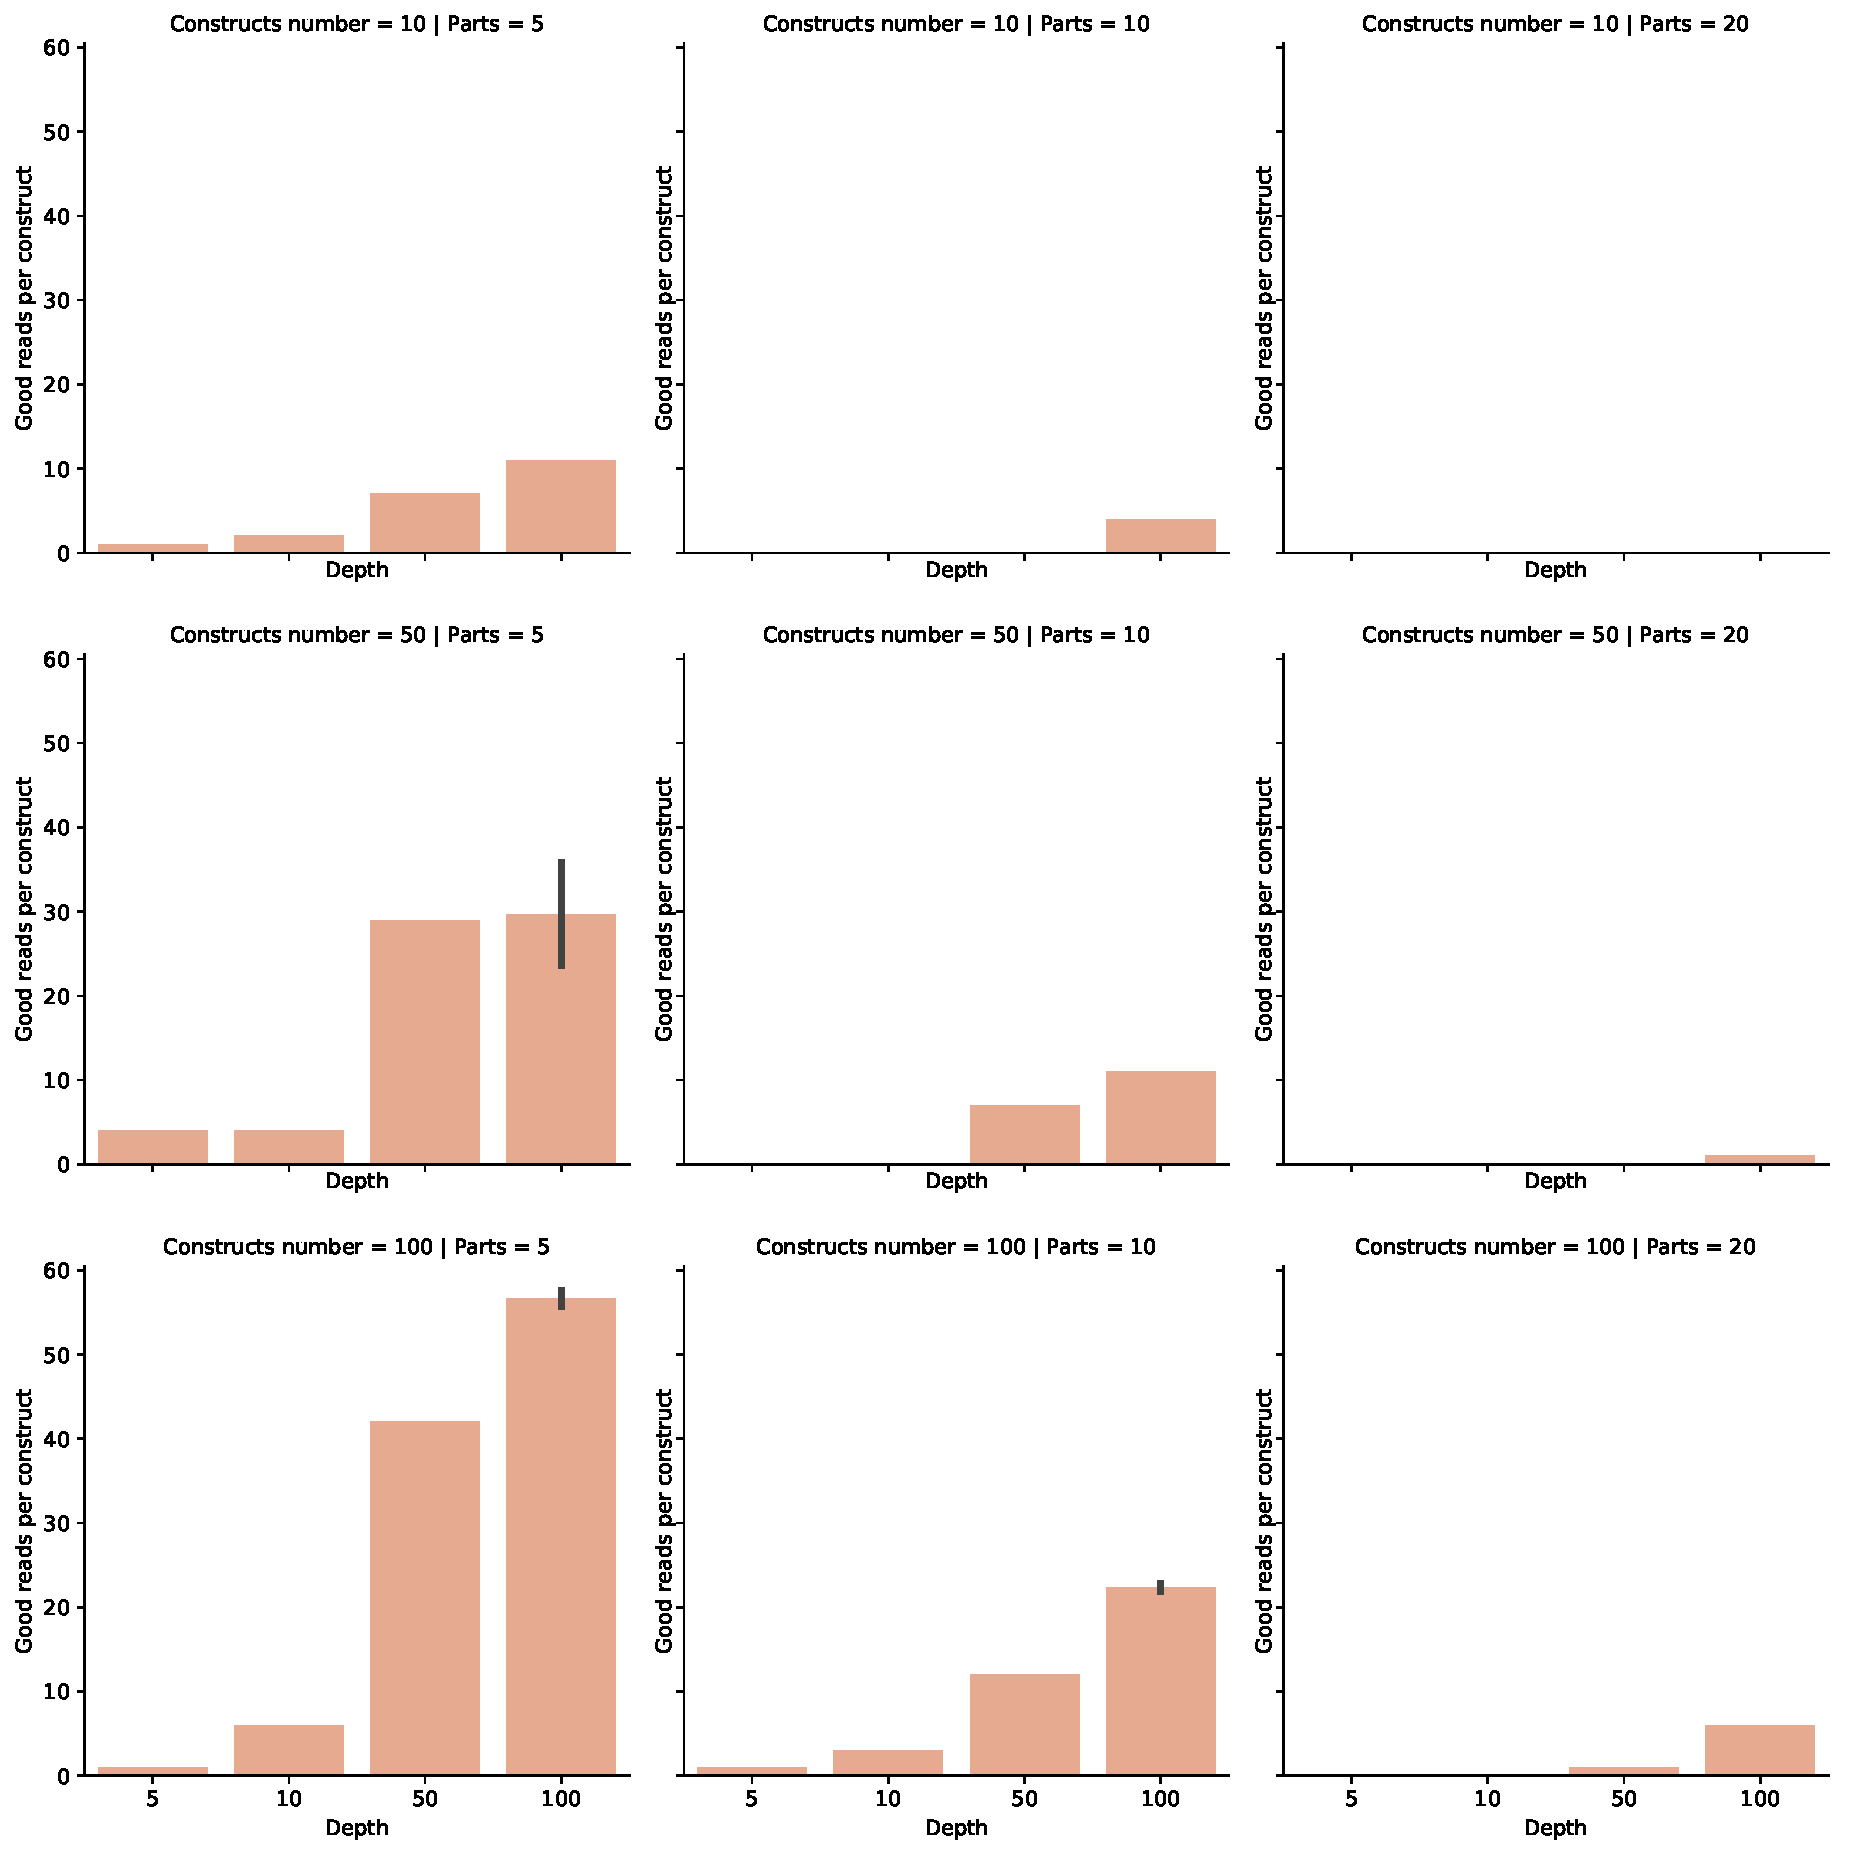
\includegraphics[width=1\textwidth]{../results/images_notebook/v_322/100_good_reads_plot.pdf}
    \end{center}
    \caption{{\bf good reads $100\%$}}
   \label{fig:v_322_good_reads_100}
\end{figure}


\subsubsection{Good reads ratio}
Given by good $reads / all reads$
Evaluating amount of good reads
\textbf{Good reads} = the number of reads with a length $\geq$ of $99\%$ of the orignal construct

\begin{figure}[ht]
    \begin{center}
    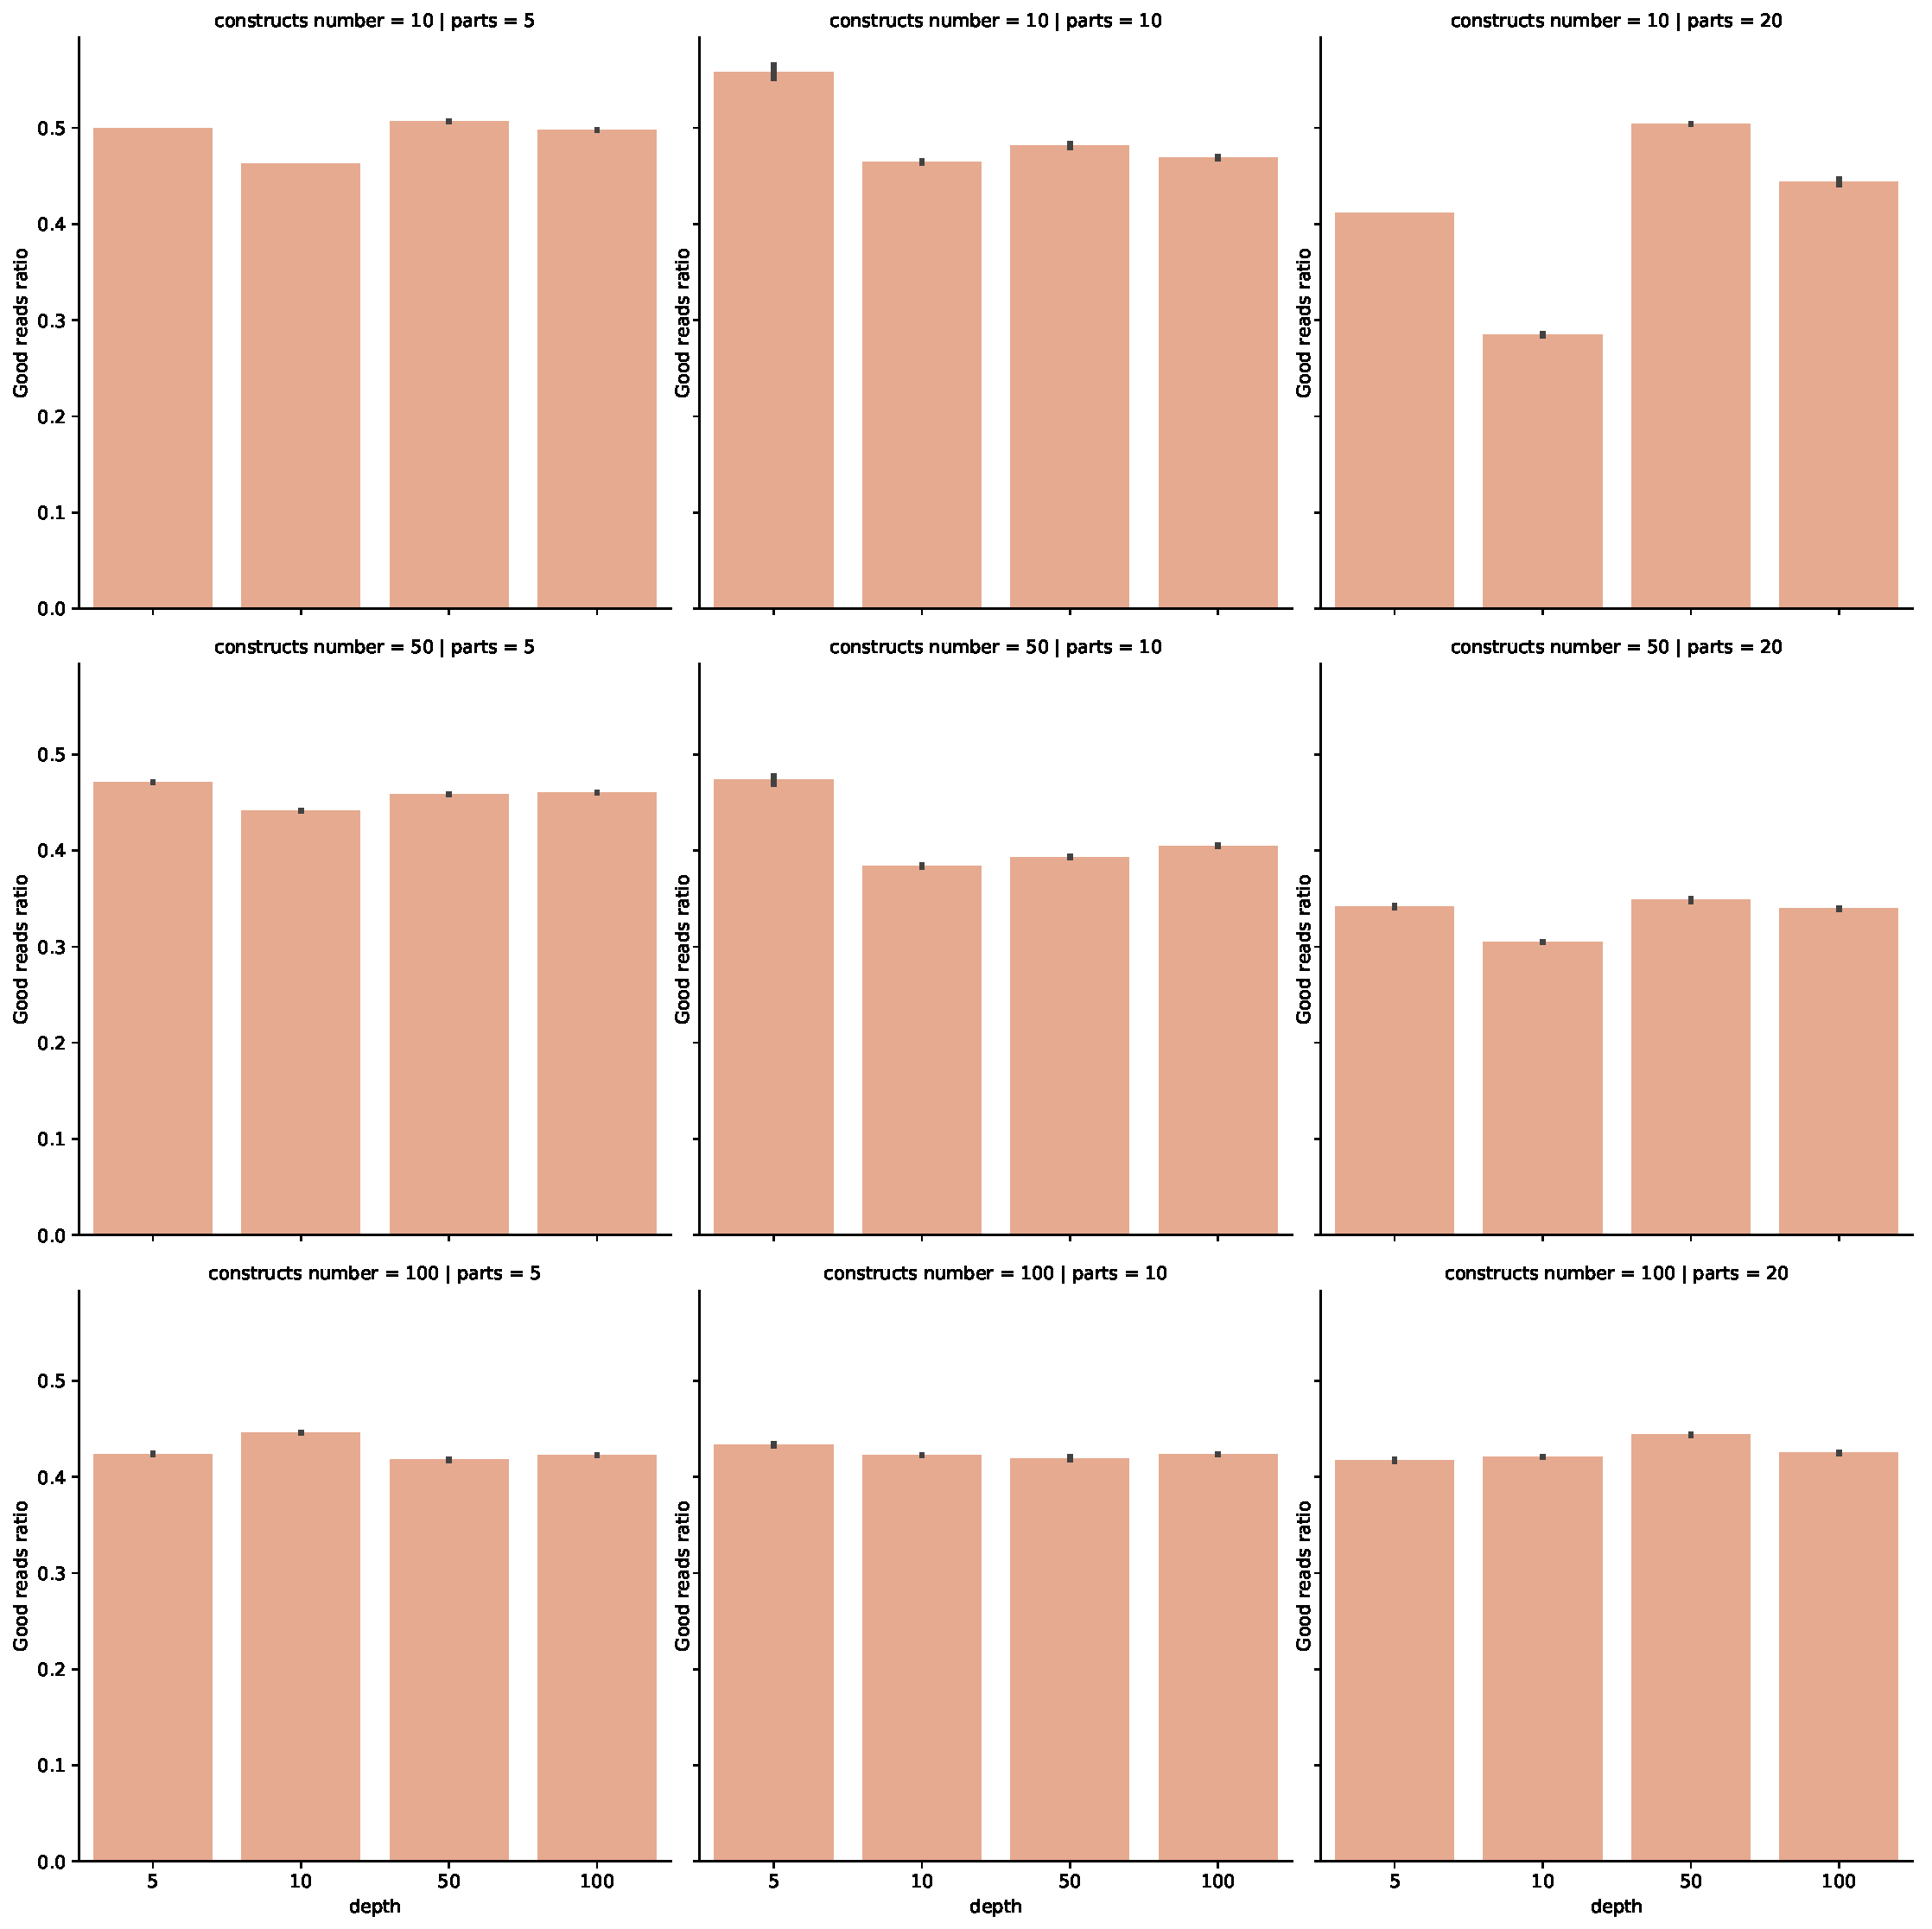
\includegraphics[width=1\textwidth]{../results/images_notebook/v_322/99_good_reads_ratio.pdf}
    \end{center}
    \caption{{\bf good reads ratio $99\%$}}
   \label{fig:v_322_good_reads_ratio_99}
\end{figure}

\begin{figure}[ht]
    \begin{center}
    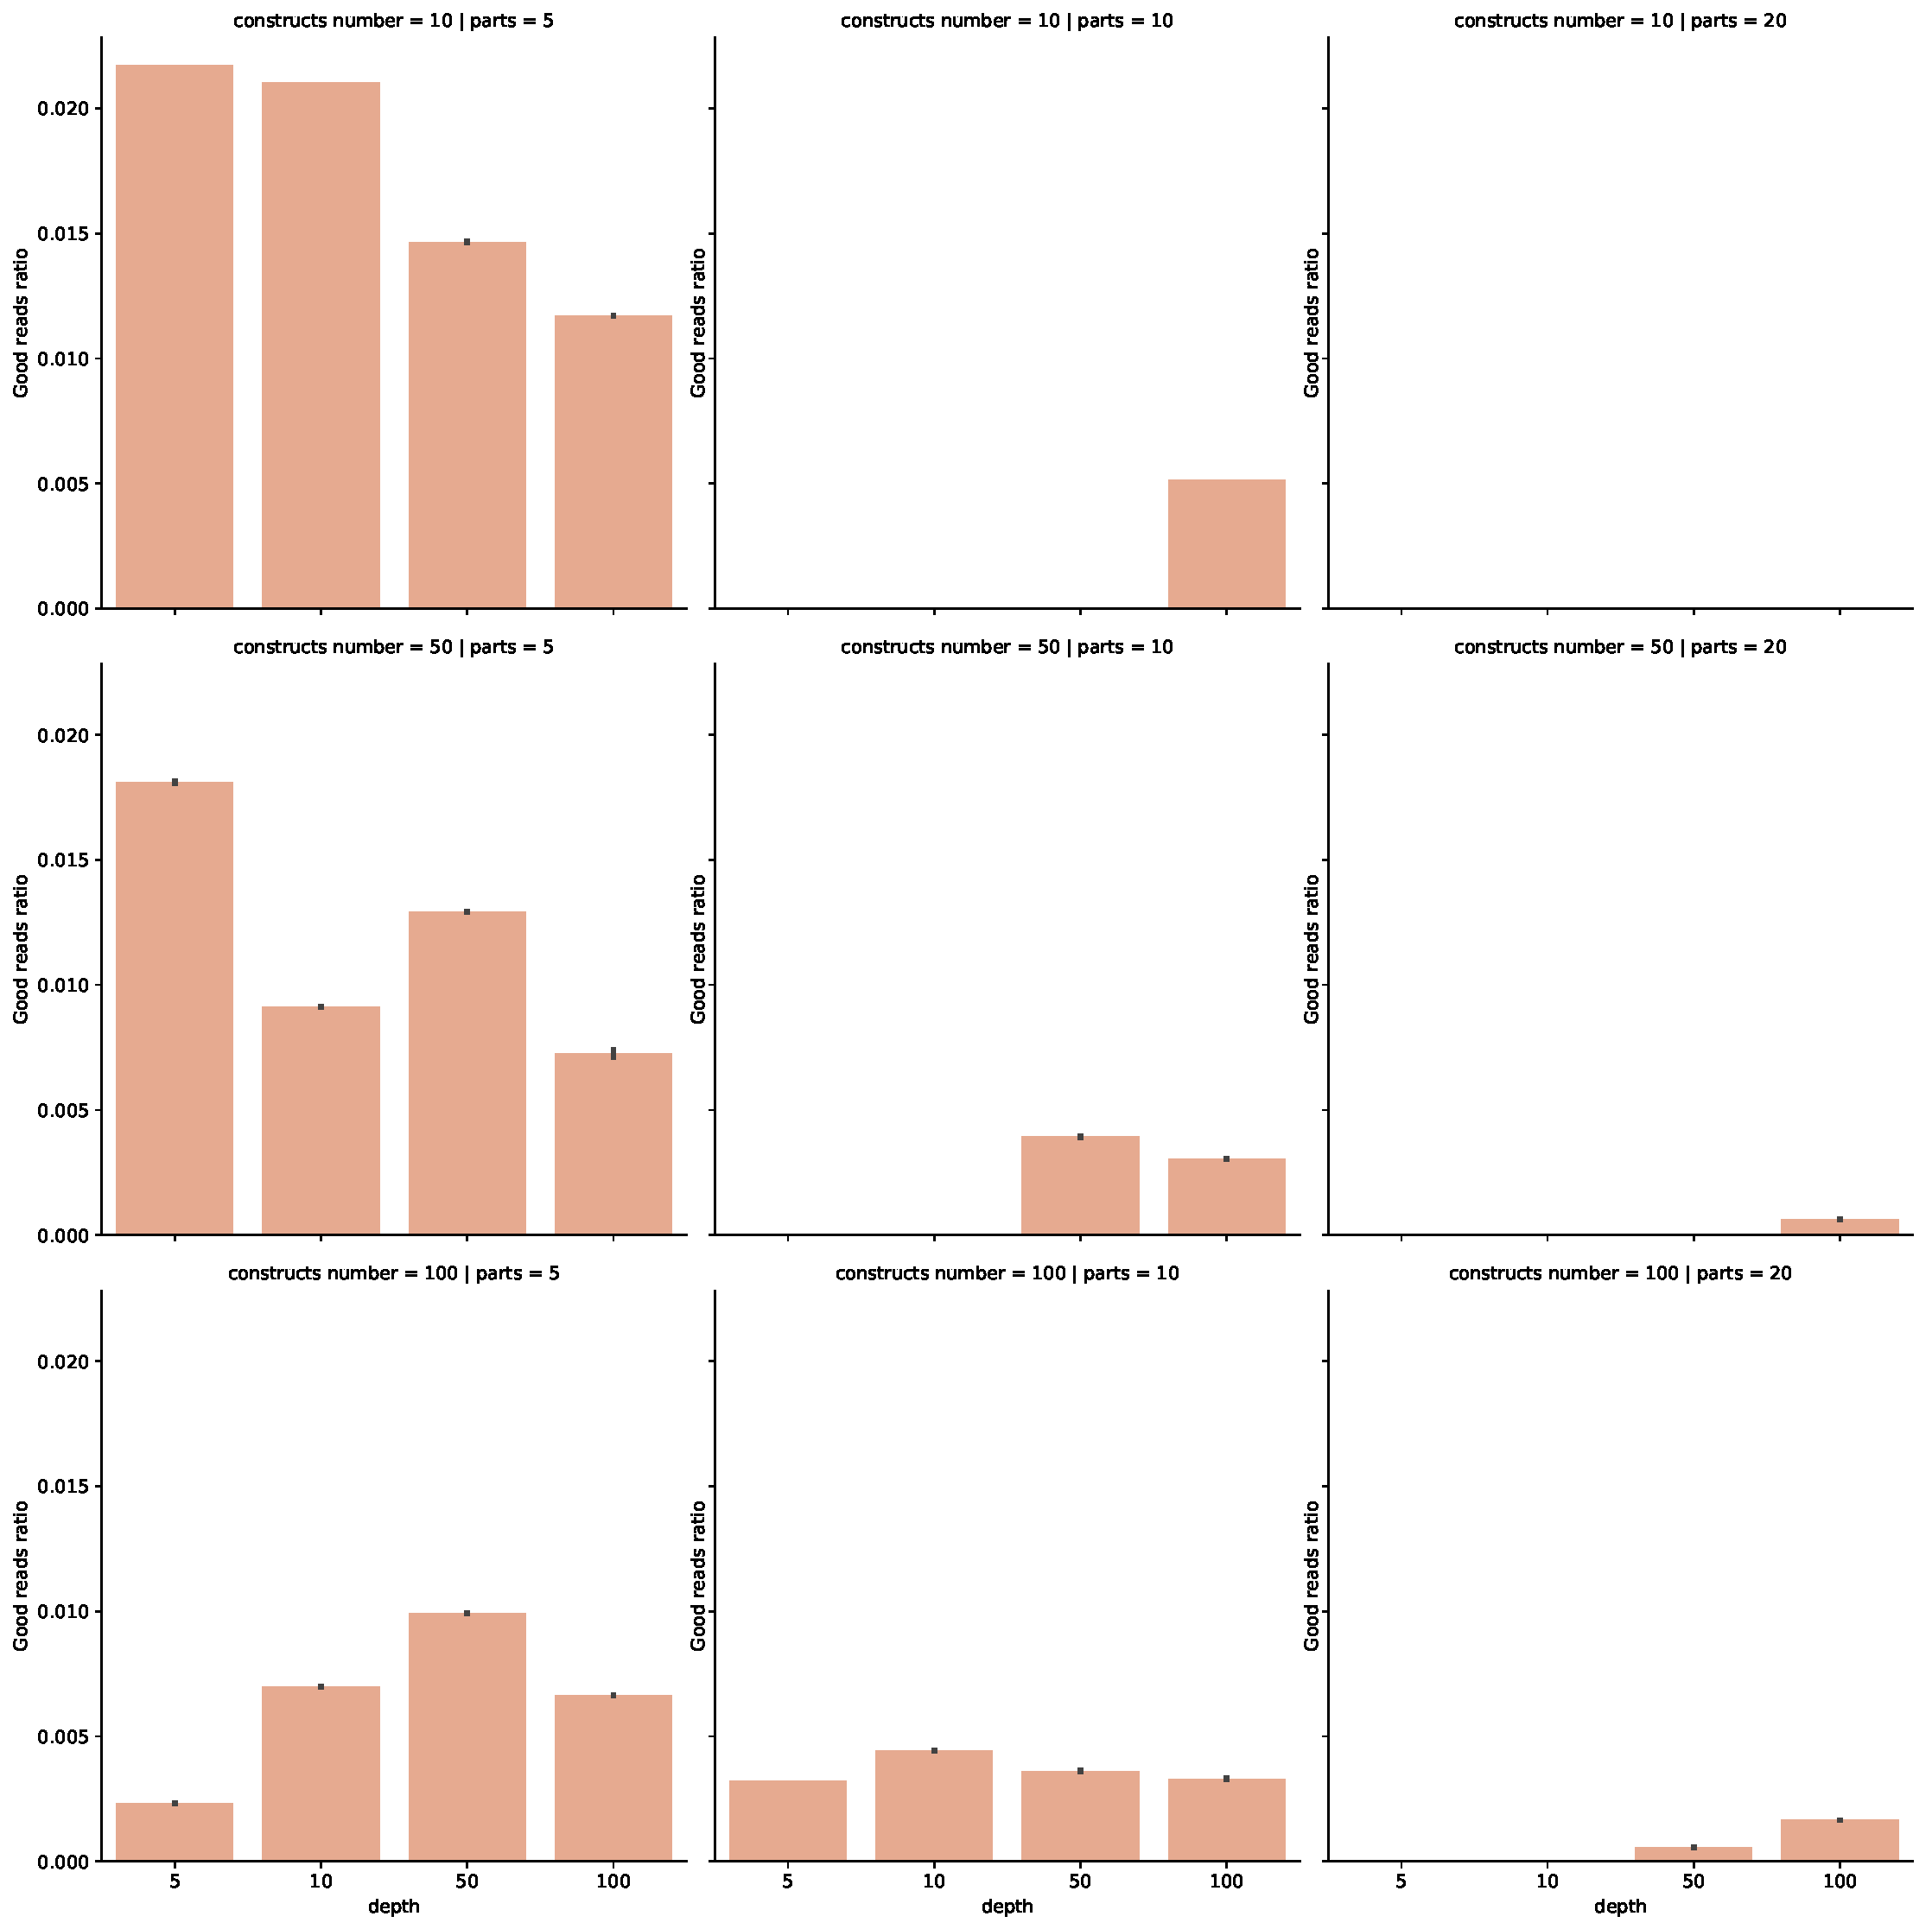
\includegraphics[width=1\textwidth]{../results/images_notebook/v_322/100_good_reads_ratio.pdf}
    \end{center}
    \caption{{\bf good reads ratio $100\%$}}
   \label{fig:v_322_good_reads__ratio_100}
\end{figure}

\clearpage
\subsection{V3.4.0 }
Results in this section can be obtained by running the following pipeline:
\begin{lstlisting}[language=Python]
    project: "mn_similarity_00"
    genbank: "yeast_chromosome_xiv.gb"
    run: 10

    generate_testbeds:
        cds_number : 50
        constructs_number: [10,50,100]
        parts : [5,10,20]
        constructs_similarity : 0.0
        parts_similarity : 0.0
        mutation_method : "last"

    badreads:
        quantity : [5x,10x,50x,100x]
        error_model: "nanopore"
        qscore_model: "nanopore"
        glitches: "0,0,0"
        junk_reads: 0
        random_reads: 0
        chimeras: 0
        identity: 95,100,4
        start_adapter_seq: ' "" '
        end_adapter_seq: ' "" '

    nanogate:
        error_rate : ["001","010","030"]
        jaccard_thresholds: ["00"]
\end{lstlisting}
\clearpage

\subsubsection{nanogate accuracy}
Accuracy is defined as:
$Good reads true postives/ good reads$
\textbf{Good reads} = the number of reads with a length $\geq$ of $99\%$ of the orignal construct
\textbf{Good reads true positives} = \textbf{Good reads} matching with the expected parts in the orignal construct

\begin{figure}[ht]
    \begin{center}
    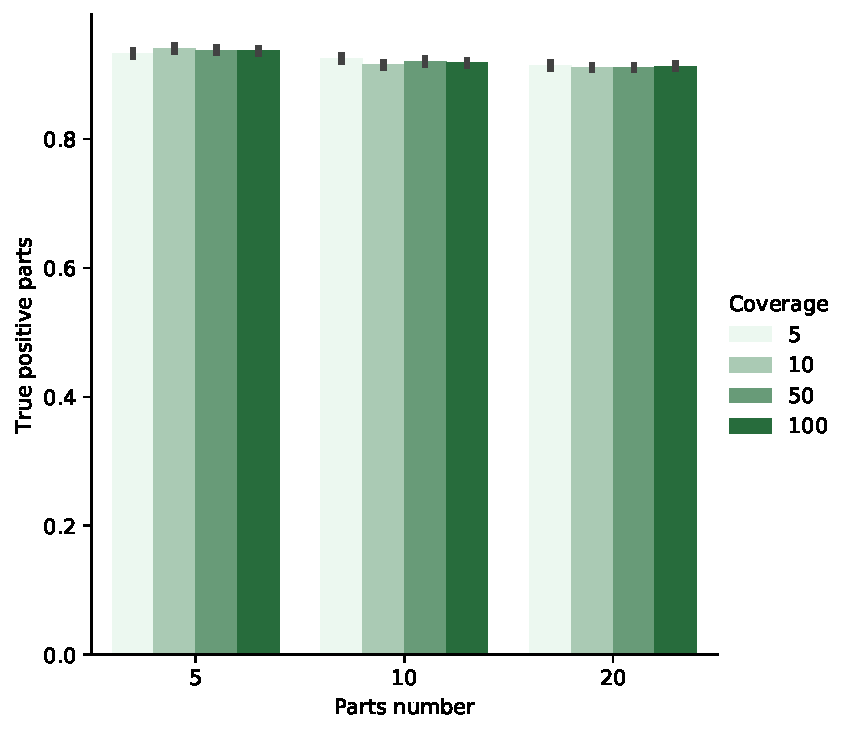
\includegraphics[width=1\textwidth]{../results/images_notebook/v_340/00_minimap2_true_positive.pdf}
    \end{center}
    \caption{{\bf  minimap2 accuracy similarity 0}This plot includes only alignment with alignment alignment score.
    original reference are aligned to the reads }
   \label{fig:v_340_minimap_accuracy_sim_0}
\end{figure}


\begin{figure}[ht]
    \begin{center}
    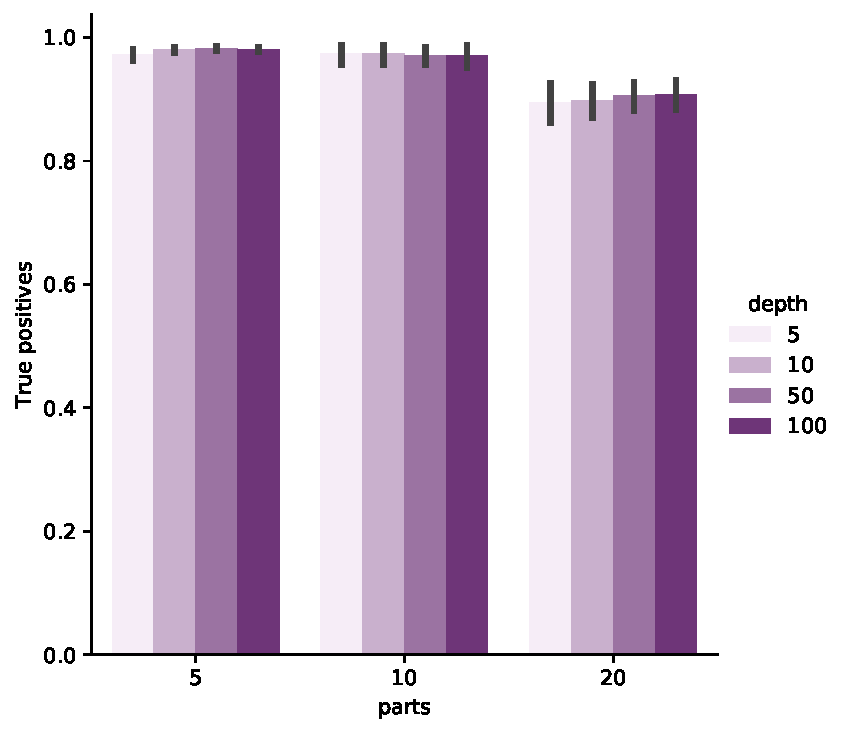
\includegraphics[width=1\textwidth]{../results/images_notebook/v_340/00_nanogate_good_reads_true_positves.pdf}
    \end{center}
    \caption{{\bf nanogate accuracy similarity 0} This plot takes into account only reads with a length >= $99\%$ of the
    original construct length }
   \label{fig:v_340_nanogate_accuracy_sim_0}
\end{figure}


\begin{figure}[ht]
    \begin{center}
    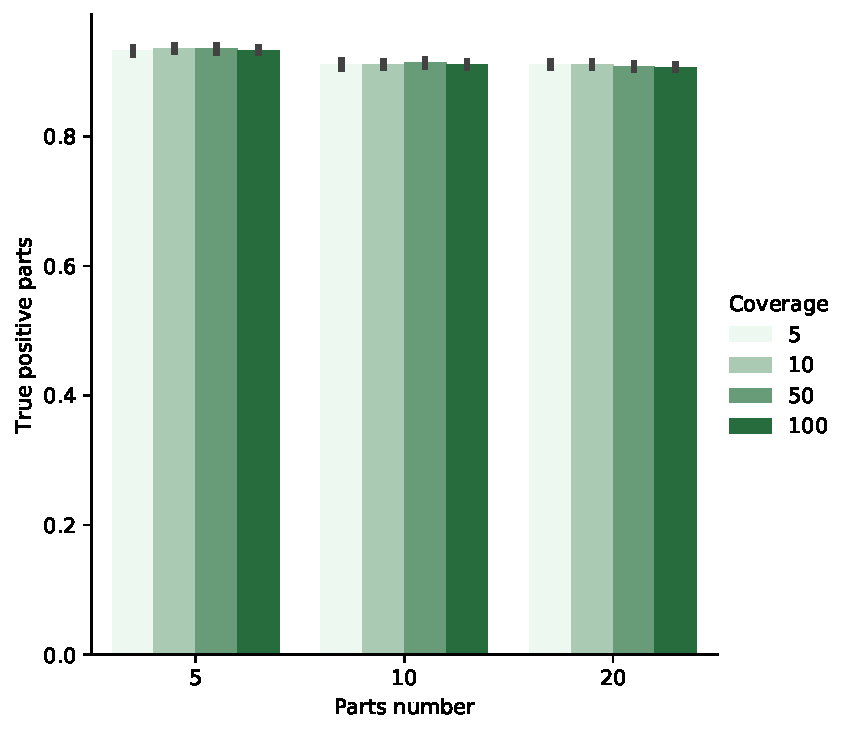
\includegraphics[width=1\textwidth]{../results/images_notebook/v_340/70_minimap2_true_positive.pdf}
    \end{center}
    \caption{{\bf  minimap2 accuracy similarity 70}This plot includes only alligment with alignment alignment score.
    original reference are aligned to the reads }
   \label{fig:v_340_minimap_accuracy_sim_70}
\end{figure}

\begin{figure}[ht]
    \begin{center}
    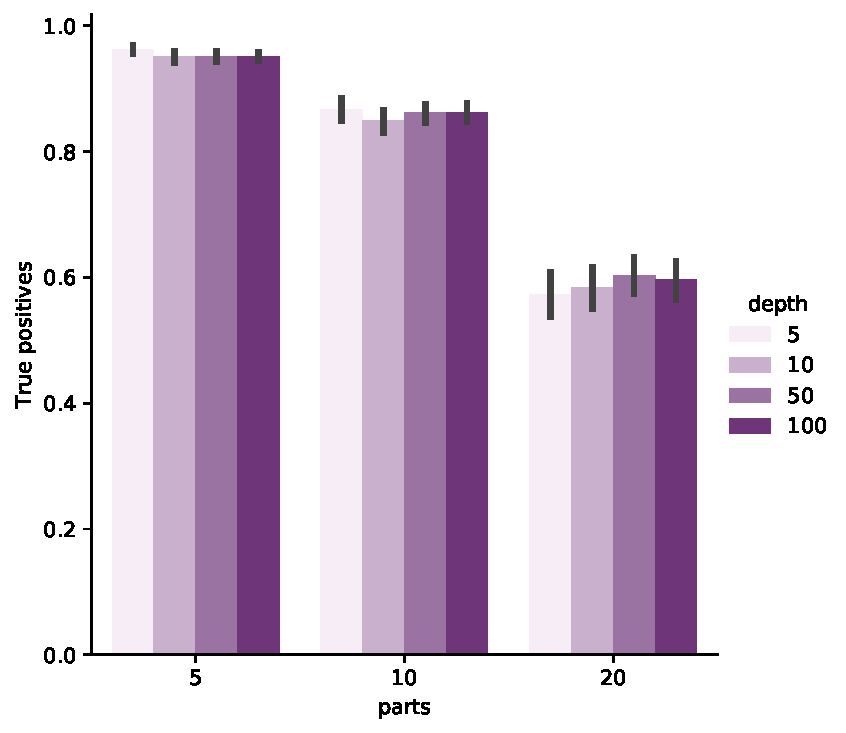
\includegraphics[width=1\textwidth]{../results/images_notebook/v_340/70_nanogate_good_reads_true_positves.pdf}
    \end{center}
    \caption{{\bf nanogate accuracy similarity 70} This plot takes into account only reads with a length >= $99\%$ of the
    original construct length }
   \label{fig:v_340_nanogate_accuracy_sim_70}
\end{figure}

\clearpage
\subsection{V4.0.0 }
Results in this section can be obtained by running the following pipeline:
\begin{lstlisting}[language=Python]
    project: "mn_similarity_00"
    genbank: "yeast_chromosome_xiv.gb"
    run: 10
    
    generate_testbeds:
        cds_number : 30
        constructs_number: [10,50,100]
        parts : [5,10,20]
        constructs_similarity : 0.0
        parts_similarity : 0.0
        mutation_method : "last"
    
    badreads:
        quantity : [5x,10x,50x,100x]
        error_model: "nanopore"
        qscore_model: "nanopore"
        glitches: "0,0,0"
        junk_reads: 0
        random_reads: 0
        chimeras: 0
        identity: 95,100,4
        start_adapter_seq: ' "" '
        end_adapter_seq: ' "" '
    
    combinatorial_assembly:
        max_parts: 5
    
    nanogate:
         error_rate : ["001","010","030"]
         jaccard_thresholds: ["00"]

\end{lstlisting}
\subsubsection{Minimap2}
Plots in this section are related  to minimap2

\begin{figure}[ht]
    \begin{center}
    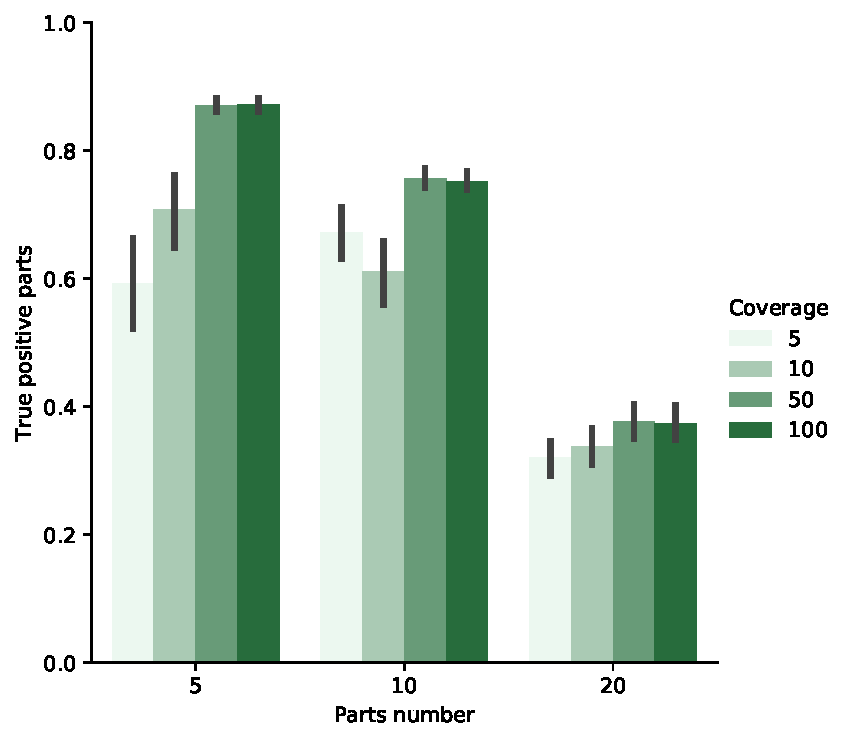
\includegraphics[width=1\textwidth]{../results/images_notebook/v_400/minimap_sim_00_true_positive.pdf}
    \end{center}
    \caption{{\bf  minimap2 true postives rate without parts similarity.} This plot shows the percentage of reads correctly analysed by Minimap2, unmapped reads and alignments without alignment score are considered as well(combinatorial assembly is not considered here)}
   \label{fig:v_400_accuracy_sim_0}
\end{figure}





\begin{figure}[ht]
    \begin{center}
    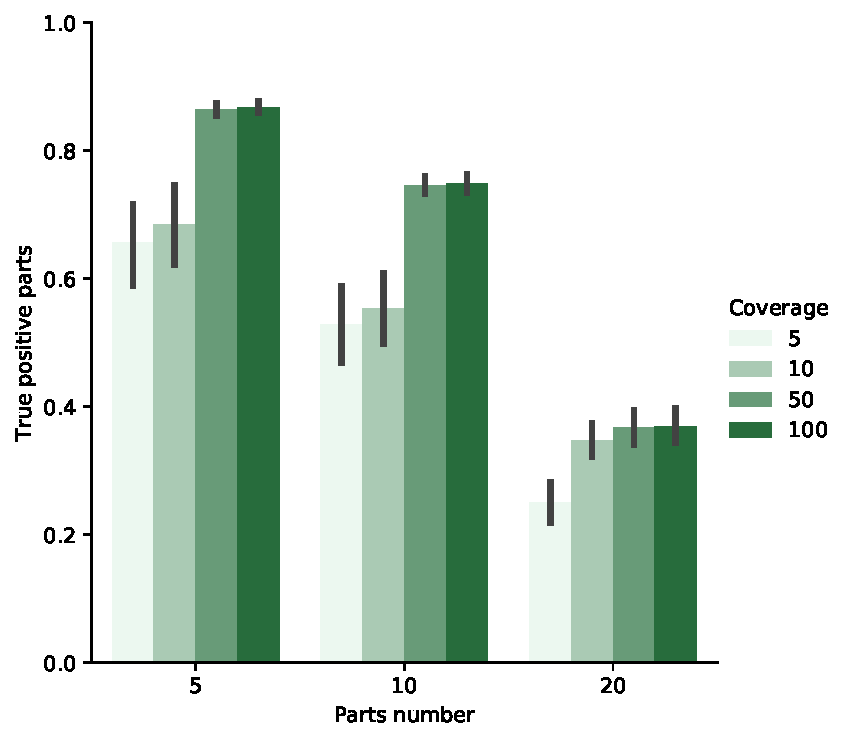
\includegraphics[width=1\textwidth]{../results/images_notebook/v_400/minimap_sim_70_true_positive.pdf}
    \end{center}
    \caption{{\bf  minimap2 true positives rate with parts similarity = 70\%.} This plot shows the percentage of reads correctly analysed by Minimap2, unmapped reads and alignments without alignment score are considered as well(combinatorial assembly is not considered here). Parts similarity slightly affect the results for Minimap2, whereas true positives rate increase with coverage and decrease with the number of parts per construct.}
   \label{fig:v_400_accuracy_sim_70}
\end{figure}

\begin{figure}[ht]
    \begin{center}
    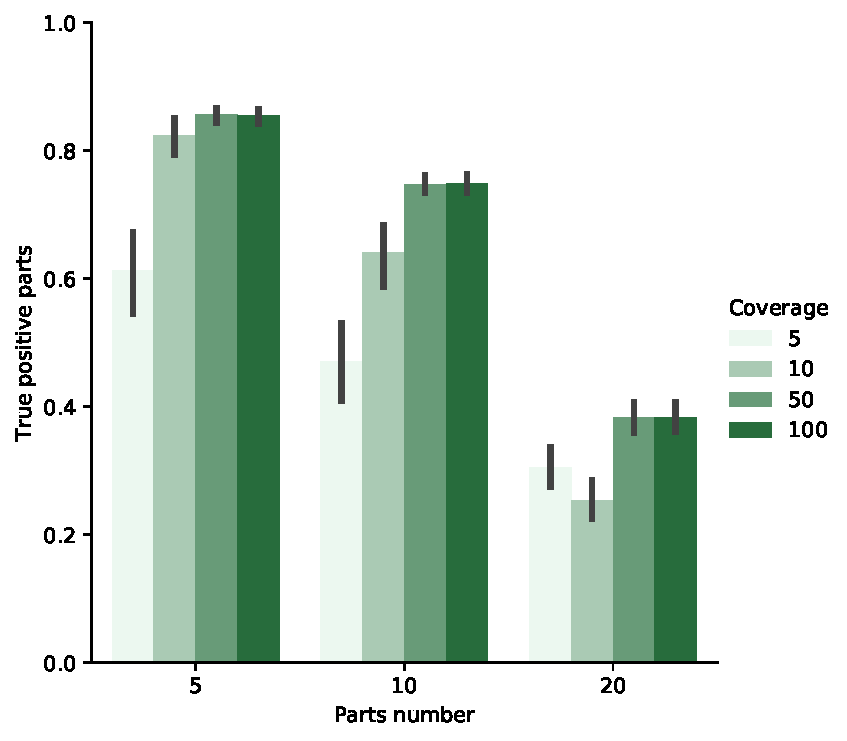
\includegraphics[width=1\textwidth]{../results/images_notebook/v_400/minimap_sim_90_true_positive.pdf}
    \end{center}
    \caption{{\bf  minimap2 accuracy with parts similarity = 90\%.} This plot shows the percentage of reads correctly analysed by Minimap2, unmapped reads and alignments without alignment score are considered as well(combinatorial assembly is not considered here). Parts similarity slightly affect the results for Minimap2, whereas true positives rate increase with coverage and decrease with the number of parts per construct.}
   \label{fig:v_400_accuracy_sim_90}
\end{figure}


   \begin{figure}[ht]
    \begin{center}
    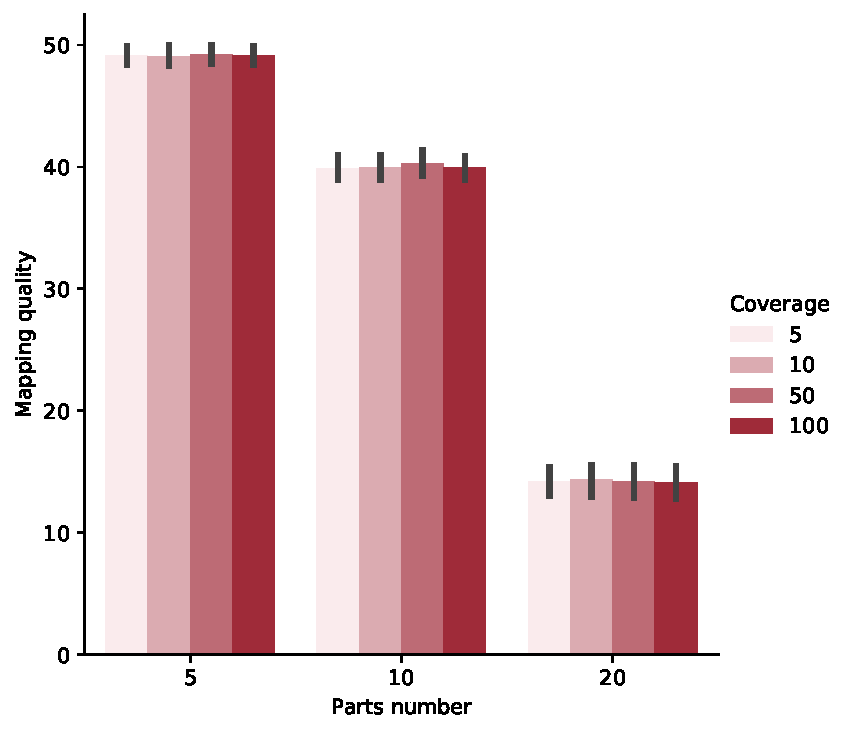
\includegraphics[width=1\textwidth]{../results/images_notebook/v_400/minimap_sim_00_mapping_quality.pdf}
    \end{center}
    \caption{{\bf  minimap2 mapping quality without parts similarity.} This plot shows how the Minimap2 mapping quality vary with coverage and number of parts per construct (combinatorial assembly is not considered here).Coverage seem to not affect mapping quality, however it decrease with the number of parts per construct}
   \label{fig:v_400_mapping_quality_sim_0}
\end{figure}

  \begin{figure}[ht]
    \begin{center}
    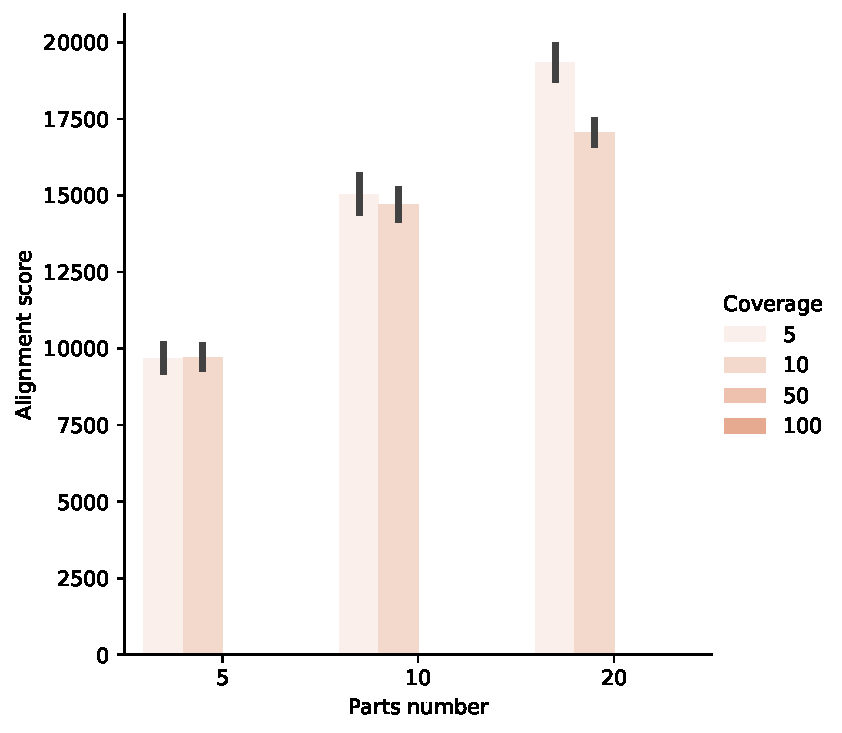
\includegraphics[width=1\textwidth]{../results/images_notebook/v_400/minimap_sim_00_alignment_score.pdf}
    \end{center}
    \caption{{\bf  minimap2 alignment score without parts similarity.} This plot shows how the Minimap2 alignment score vary with coverage and number of parts per construct (combinatorial assembly is not considered here).The alignment score increase with the number of parts per constructs, since as the length of a construct increase the number of matching bases increase as well. Coverage 50 and 100 are not shown need further investigation}
   \label{fig:v_400_alignment_score_sim_0}
\end{figure}

\begin{figure}[ht]
   \begin{center}
    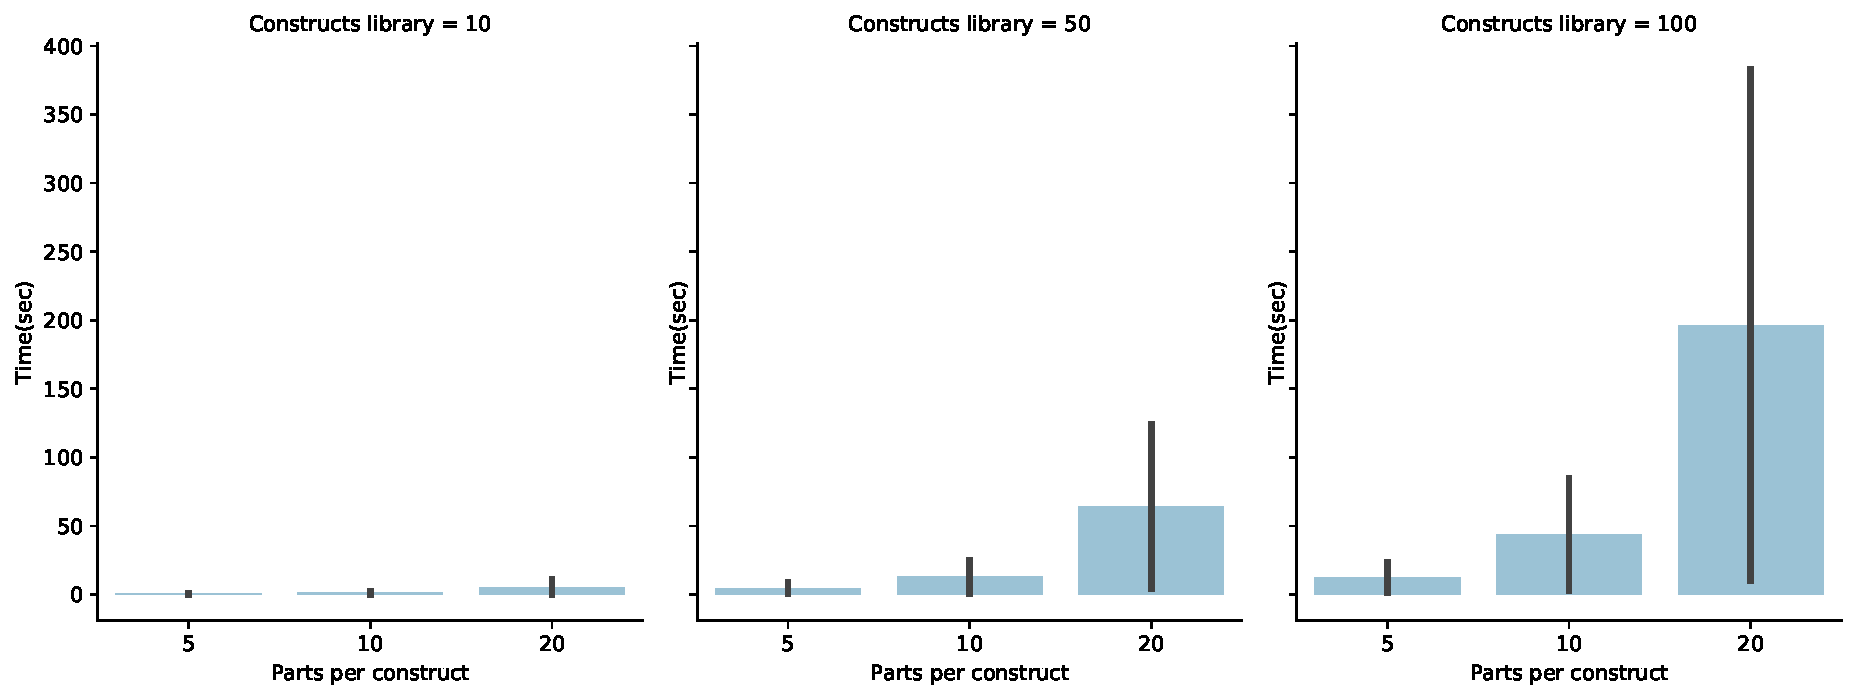
\includegraphics[width=1.35\textwidth]{../results/images_notebook/v_400/minimap_sim_00_real_time.pdf}
    \end{center}
    \caption{{\bf  minimap2 Real time without parts similarity.} This plot shows the time required by Minimap2 to per perform alignments between constructs generated by testbed generator and the reads generated by badreads tool,
    (combinatorial assembly is not considered here)}
   \label{fig:v_400_time_sim_0}
 \end{figure}

 \begin{figure}[ht]
    \begin{center}
    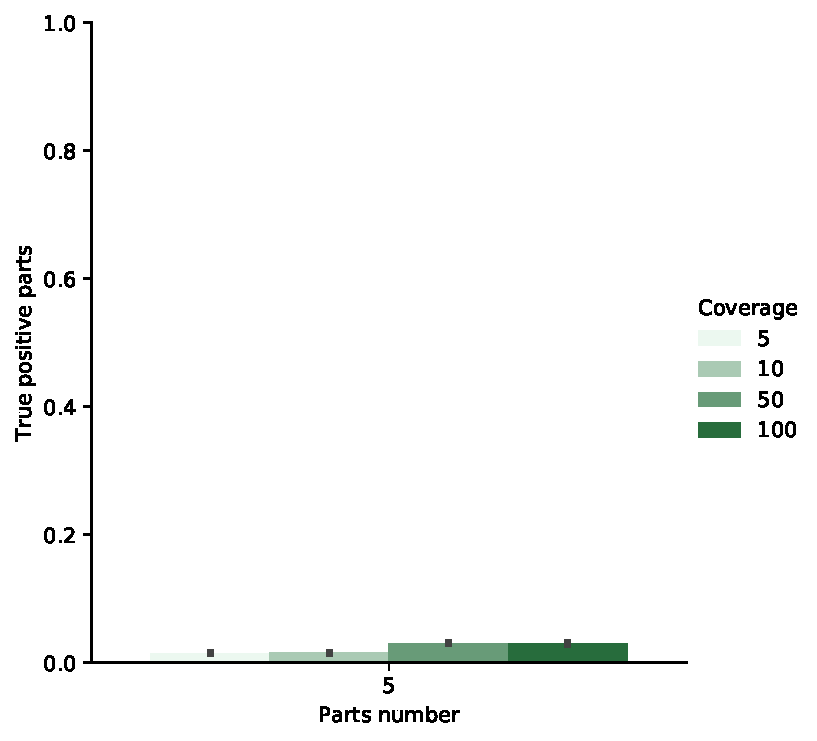
\includegraphics[width=1\textwidth]{../results/images_notebook/v_400/combinatorial_sim_00_true_positive.pdf}
    \end{center}
    \caption{{\bf  minimap2 combinatorial assembly true positives rate without parts similarity.} This plot shows the true positives rate obtained after performing an alignment between reads generated from badreads tool and parts assembled combinatorially. To save time on the analysis only combinatorial assembly for 5 parts constructs are evaluated. The true positives rate slightly increase with coverage, however is always below 0.1.  }
   \label{fig:v_400_combinatorial_sim_00}
\end{figure}
 
  \begin{figure}[ht]
    \begin{center}
    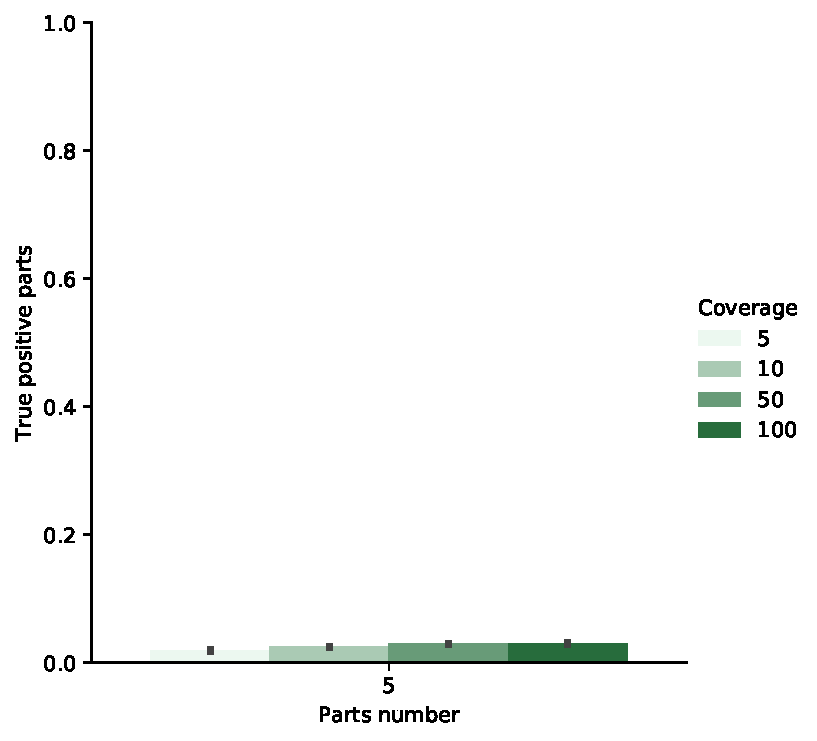
\includegraphics[width=1\textwidth]{../results/images_notebook/v_400/combinatorial_sim_90_true_positive.pdf}
    \end{center}
    \caption{{\bf  minimap2 combinatorial assembly true positives rate with parts similarity =90\%.} This plot shows the true positives rate obtained after performing an alignment between reads generated from badreads tool and parts assembled combinatorially. To save time on the analysis only combinatorial assembly for 5 parts constructs are evaluated. The true positives rate slightly increase with coverage, however is always below 0.1.  }
   \label{fig:v_400_combinatorial_sim_90}
\end{figure}

  \begin{figure}[ht]
    \begin{center}
    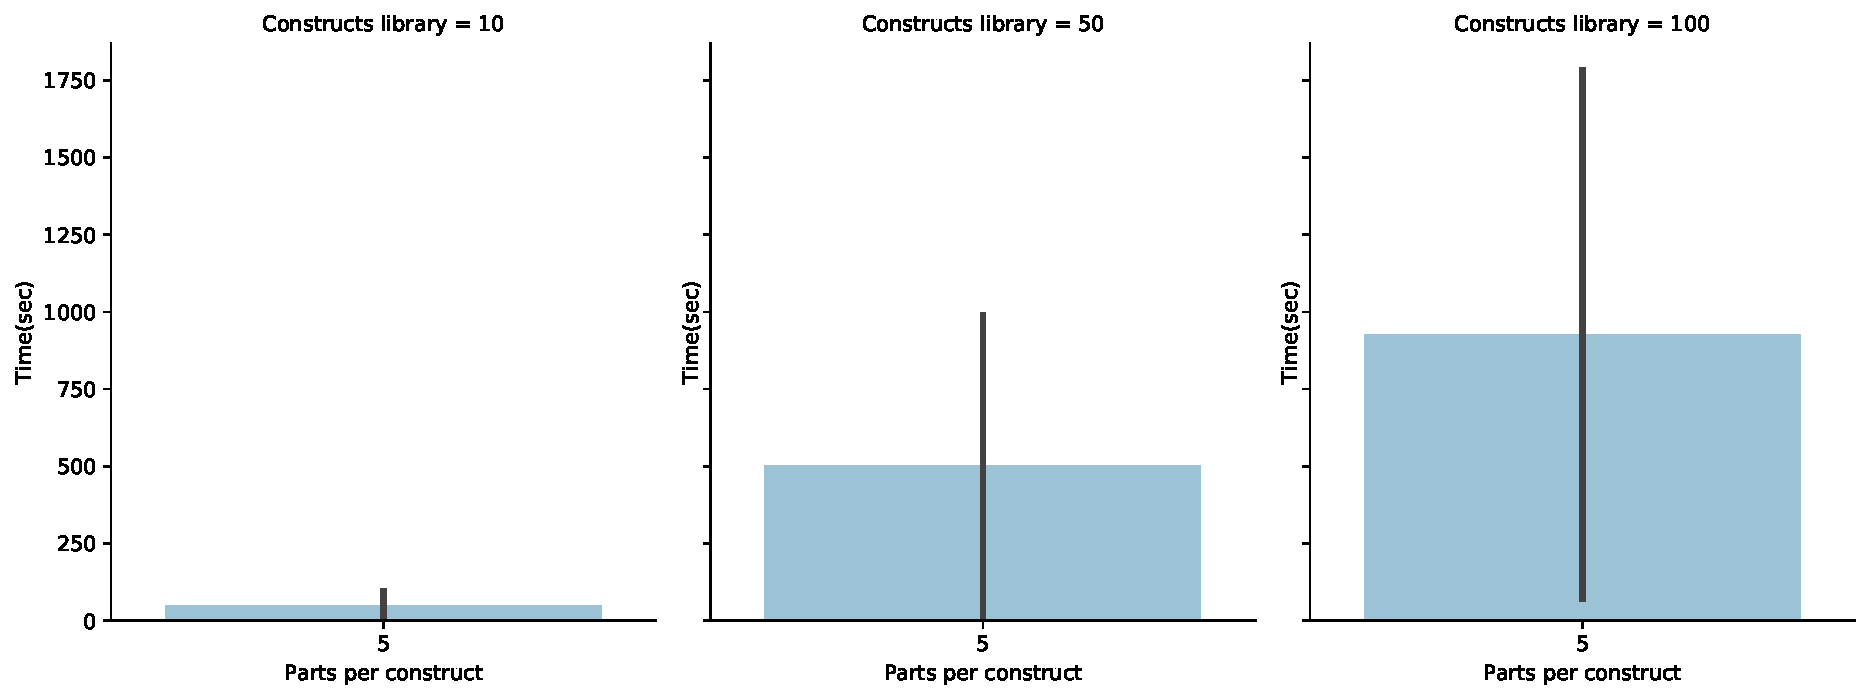
\includegraphics[width=1.35\textwidth]{../results/images_notebook/v_400/combinatorial_sim_00_real_time.pdf}
    \end{center}
    \caption{{\bf  minimap2 combinatorial assembly real time wihtout parts similarity.} This plot shows the time required by minimap2 to perform an alignment between parts combinatorially assembled used as reference and reads generated by badreas tool as query}
   \label{fig:v_400_combinatorial_sim_00_real_time}
\end{figure}
\clearpage
\subsubsection{Nanogate}


Plots in this section are related to Nanogate

\begin{figure}[ht]
    \begin{center}
    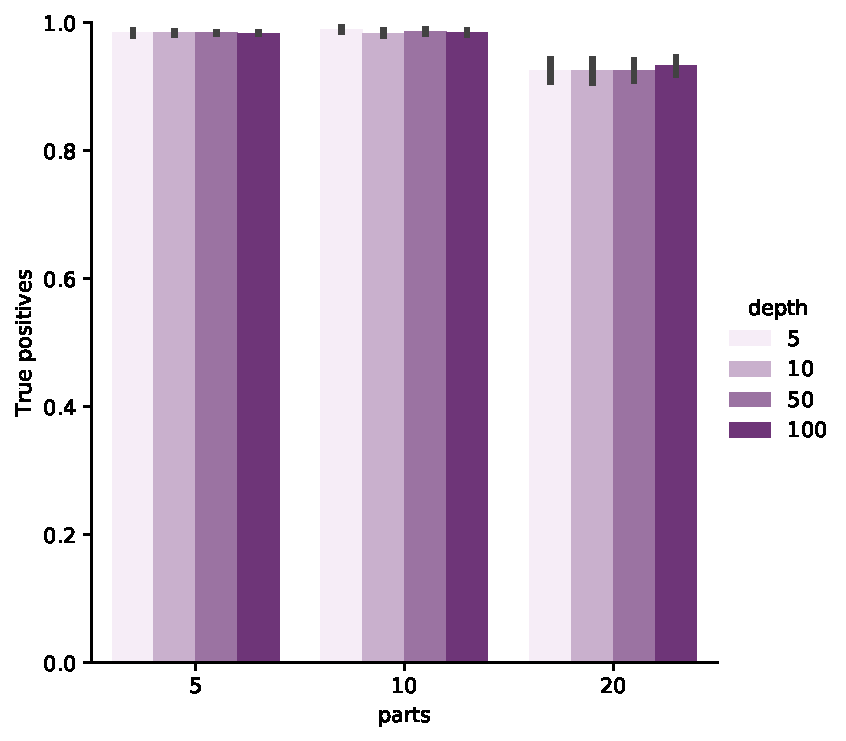
\includegraphics[width=1\textwidth]{../results/images_notebook/v_400/nanogate_sim_00_good_reads_true_positves.pdf}
    \end{center}
    \caption{{\bf  Nanogate true postives rate without parts similarity.} This plot shows the percentage of reads correctly analysed by Nanogate, only reads with a length $>=99\%$ than the constructs original length are considered here. With no parts similarity Nanogate gives a true positives rate close to 1,
    and give better result compared to Minimap2 whether in standard alignments or applied to combinatorial assembly.}
   \label{fig:v_400_nanogate_accuracy_sim_0}
\end{figure}

\begin{figure}[ht]
    \begin{center}
    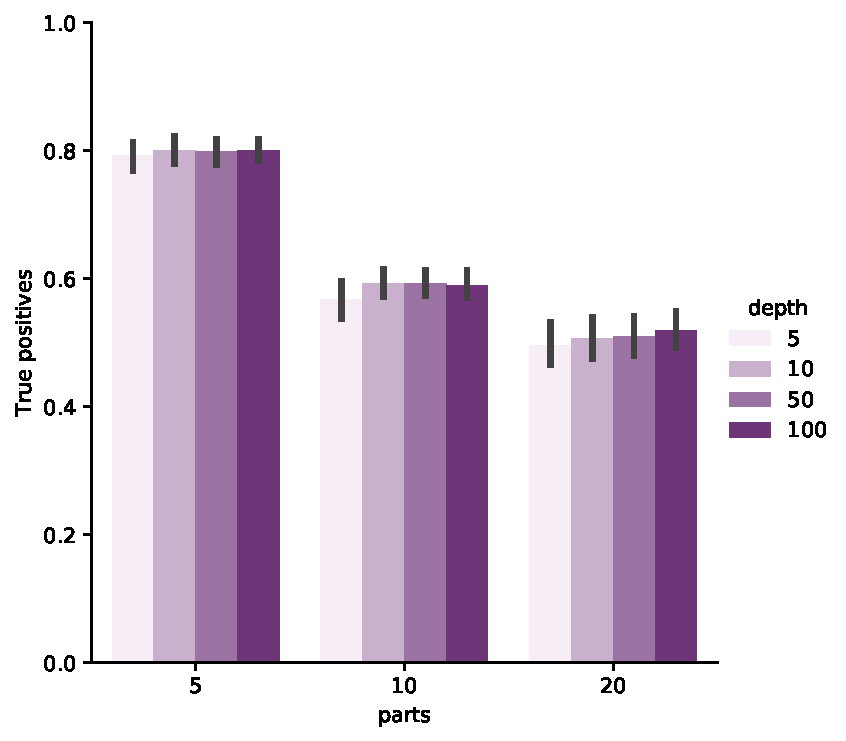
\includegraphics[width=1\textwidth]{../results/images_notebook/v_400/nanogate_sim_90_good_reads_true_positves.pdf}
    \end{center}
    \caption{{\bf  Nanogate true positives rate with parts similarity =90\%.} This plot shows the percentage of reads correctly analysed by Nanogate, only reads with a length $>=99\%$ than the constructs original length are considered here. With no parts similarity Nanogate gives a true positives rate close to 1,
    and give better result compared to Minimap2 whether in standard alignments or applied to combinatorial assembly. However, compared to analysis performed without parts similarity the true positives rate has sensibly decreased in particular for 10 and 20 parts constructs }
   \label{fig:v_400_nanogate_accuracy_sim_90}
\end{figure}

\begin{figure}[ht]
    \begin{center}
    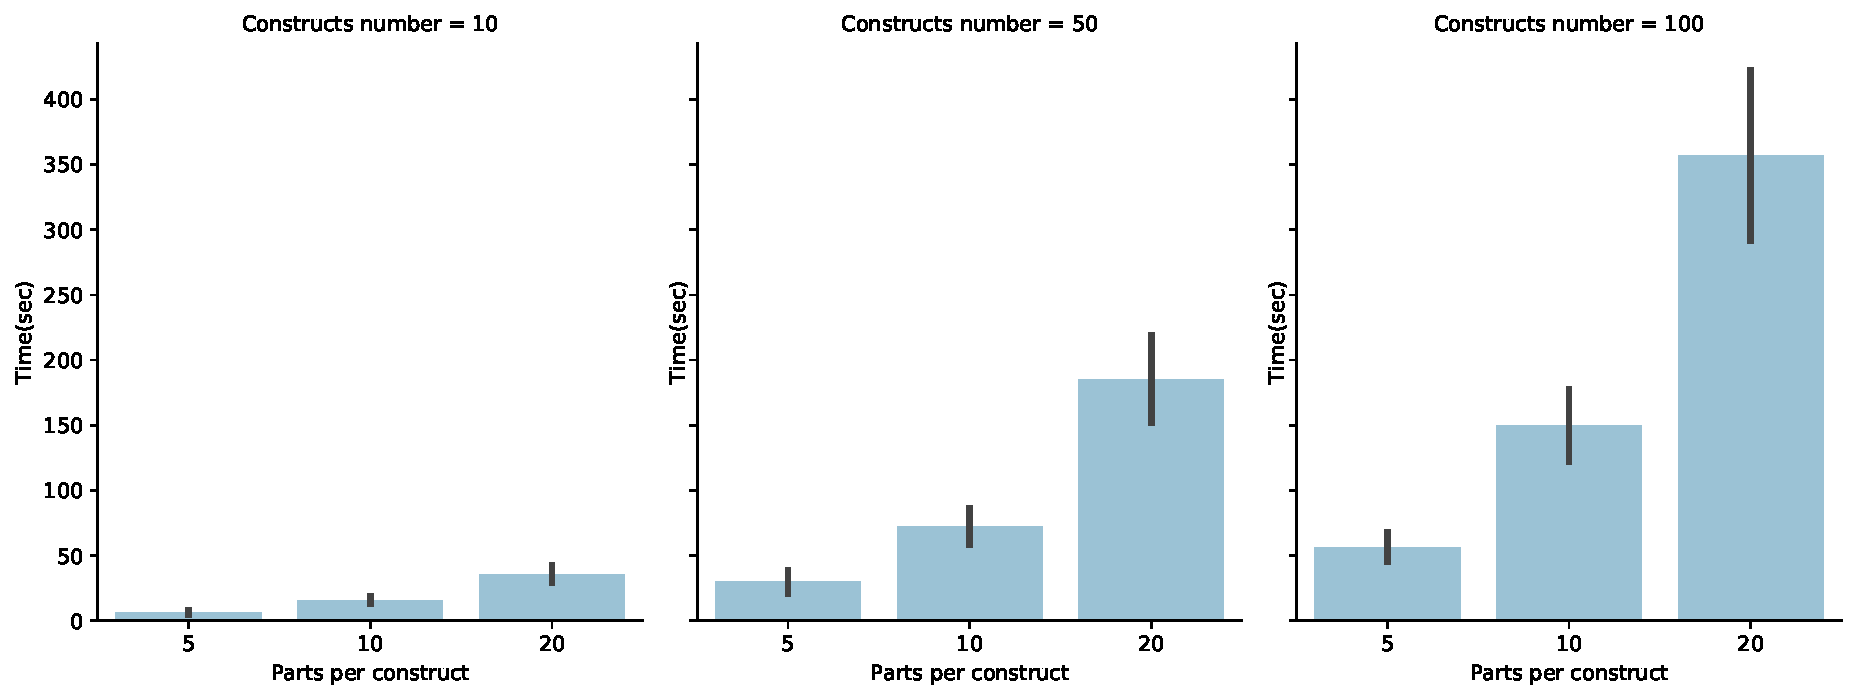
\includegraphics[width=1.35\textwidth]{../results/images_notebook/v_400/nanogate_sim_00_time_plot.pdf}
    \end{center}
    \caption{{\bf  Nanogate time plot.} This plot shows the time required by Nanogate to perform the analysis, on average if compared to Minimap2 applied in standard condition, Nanogate require on average more time to perform the analysis. If we compare the computational time bewteen Nanogate and Minimap2 applied to combinatorial assembly, Nanogate requires by far less time.   }
   \label{fig:v_400_nanogate_time_sim_00}
\end{figure}

\clearpage
\subsubsection{Minimap2 Nanogate Comparisons}
Plots in this section show comparisons between Minimpa2 and Nanogate

\begin{figure}[ht]
    \begin{center}
    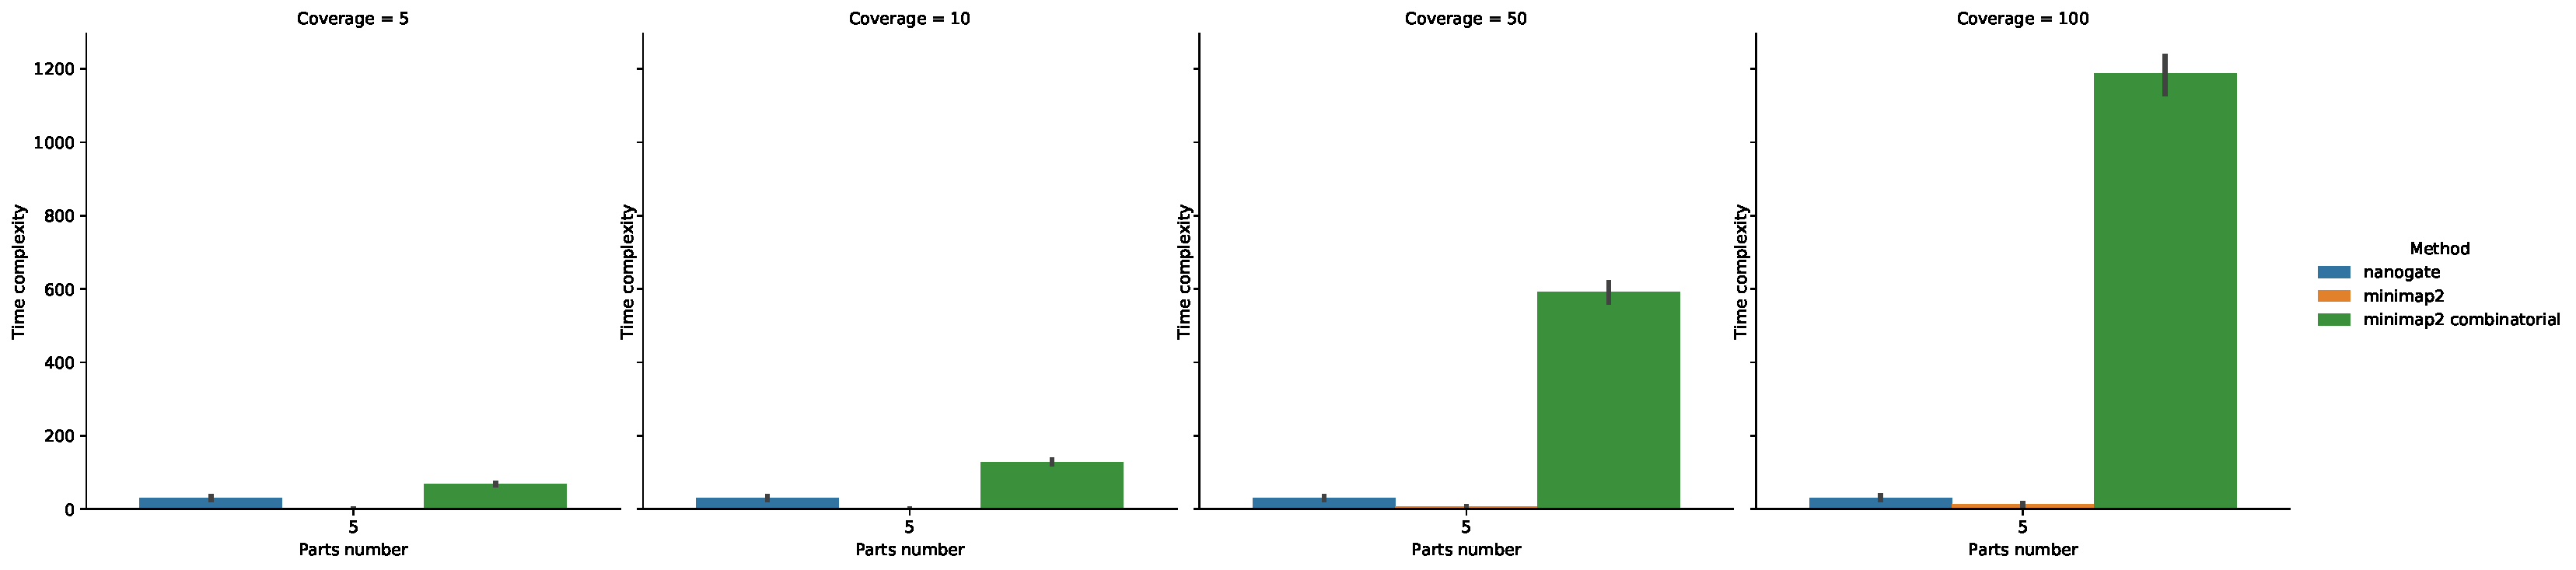
\includegraphics[width=1.35\textwidth]{../results/images_notebook/v_400/sim_00_5_parts_time_comparison.pdf}
    \end{center}
    \caption{{\bf Nanogate Minimap2 and combinatorial assembly time plot.} This plot shows, in absence of parts similarity, the time complexity comparison between Nanogate, Minimap2 using as query only constructs reads, and Minimap2 applied to combinatorial assemblies. To simplify the analysis only 5 parts constructs are taken into account.}
   \label{fig:v_400_sim_00_5_parts_time_comparison}
\end{figure}
 
 \begin{figure}[ht]
    \begin{center}
    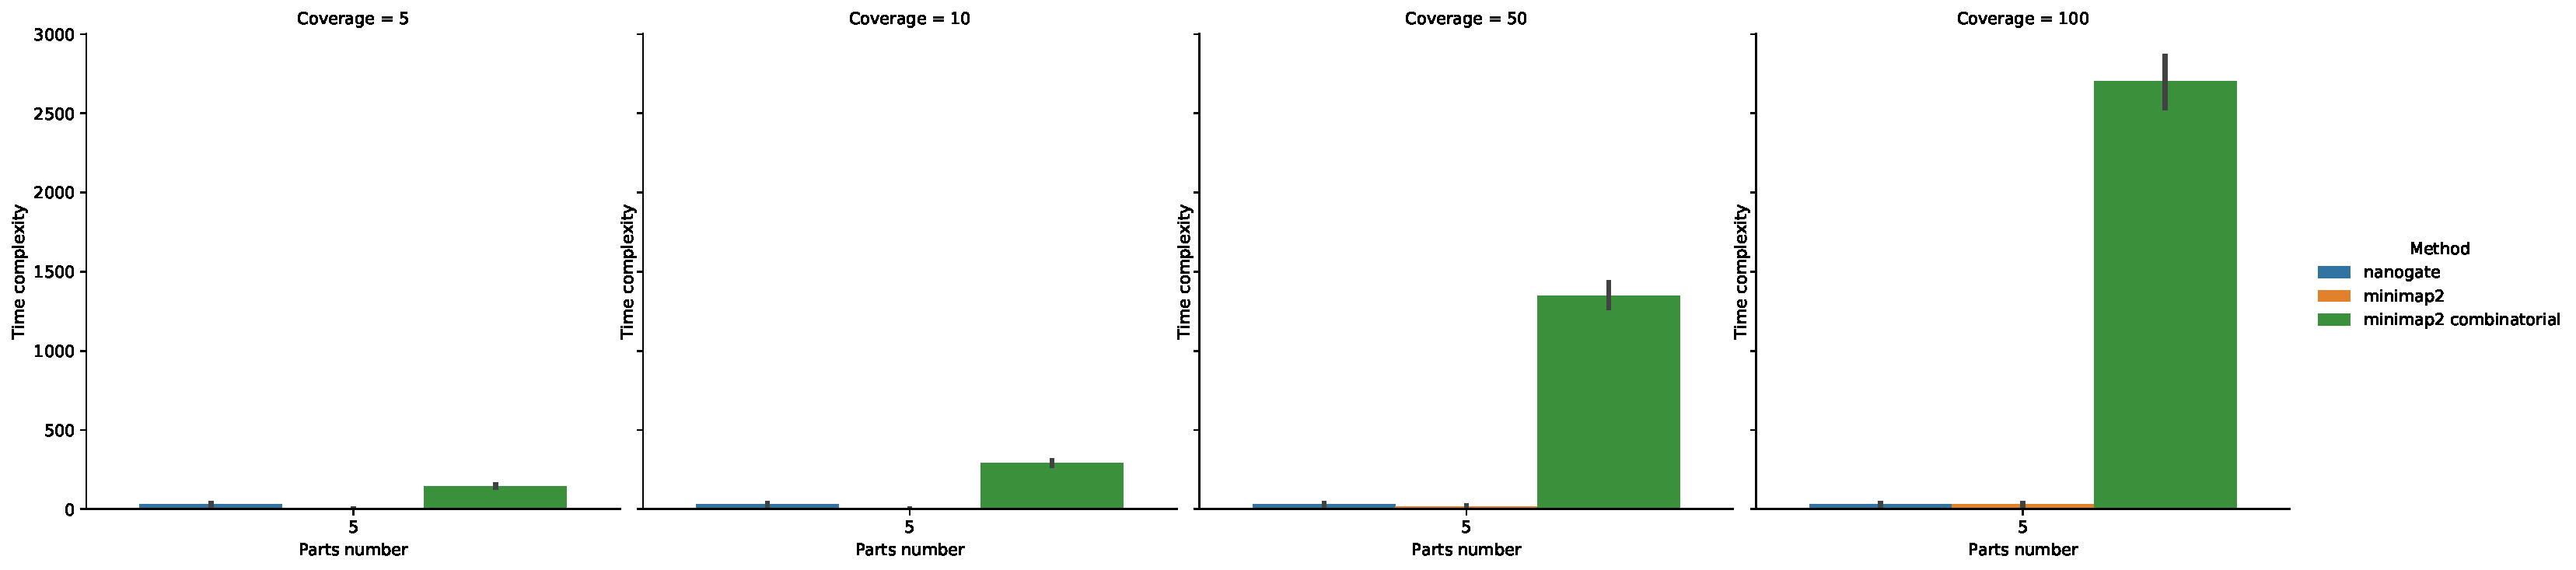
\includegraphics[width=1.35\textwidth]{../results/images_notebook/v_400/sim_09_5_parts_time_comparison.pdf}
    \end{center}
    \caption{{\bf Nanogate Minimap2 and combinatorial assembly time plot.} This plot shows, for parts similarity $=90\%$, the time complexity comparison between Nanogate, Minimap2 using as query only constructs reads, and Minimap2 applied to combinatorial assemblies. To simplify the analysis only 5 parts constructs are taken into account.}
   \label{fig:v_400_sim_09_5_parts_time_comparison}
\end{figure}



 \begin{figure}[ht]
    \begin{center}
    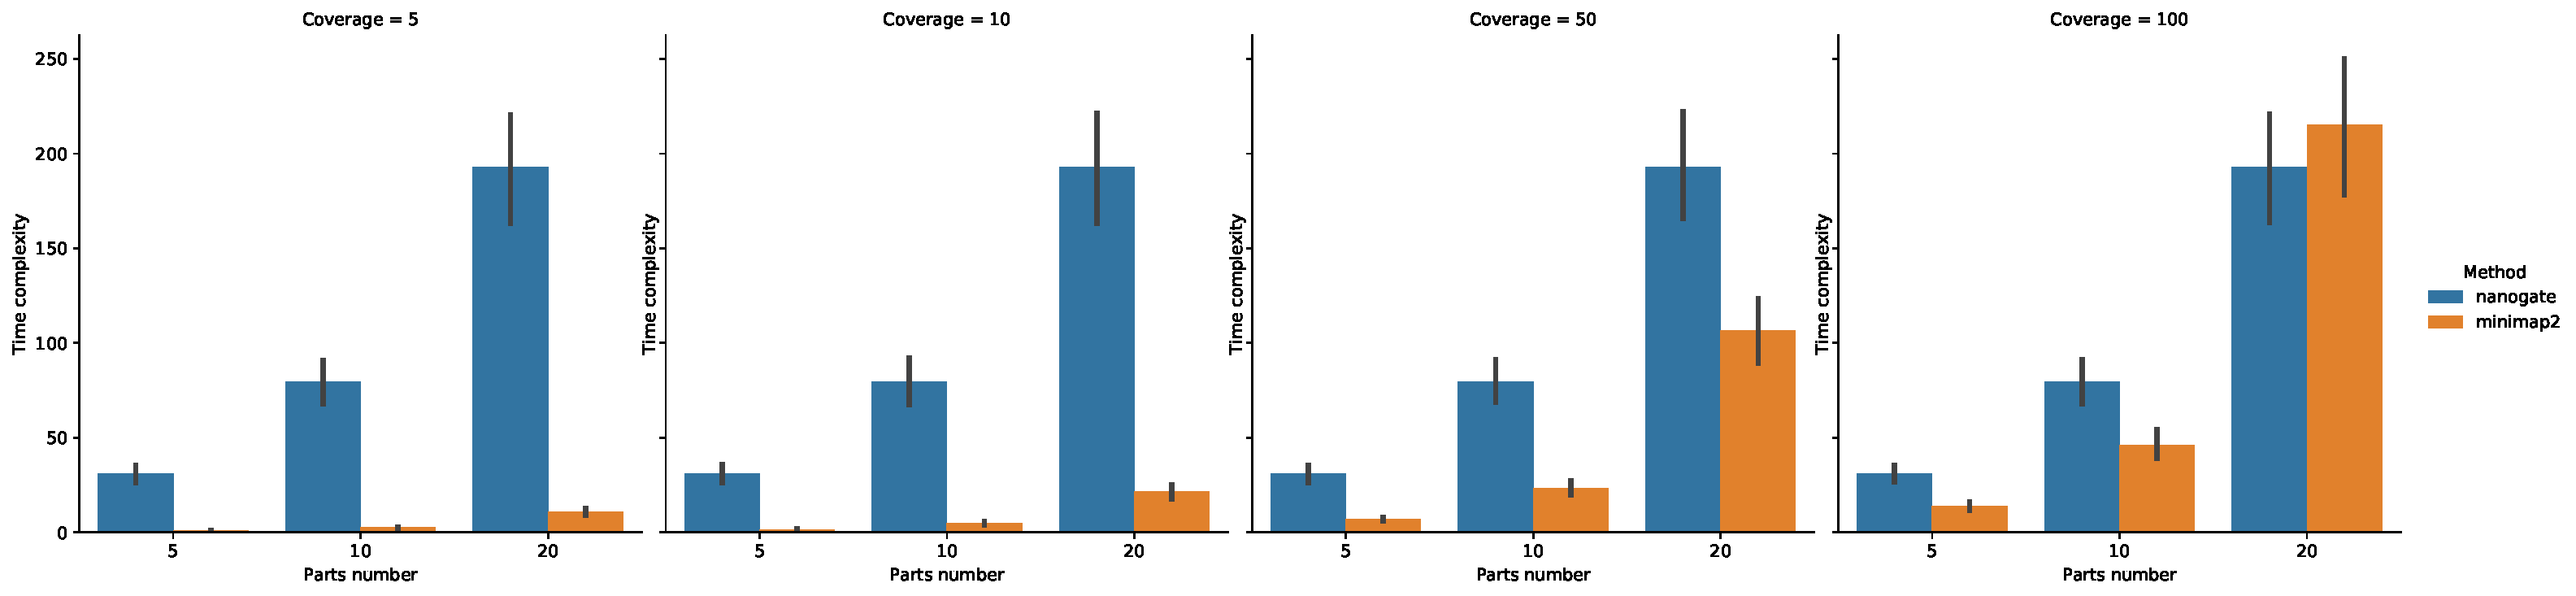
\includegraphics[width=1.35\textwidth]{../results/images_notebook/v_400/sim_00_minimap2_nanogate_time_comparison.pdf}
    \end{center}
    \caption{{\bf Nanogate and Minimap2 time comparison plot.} This plot shows, in absence of parts similarity, the time complexity comparison between Nanogate and Minimap2 using as query only constructs reads.}
   \label{fig:v_400_sim_00_time_comparison}
\end{figure}


 \begin{figure}[ht]
    \begin{center}
    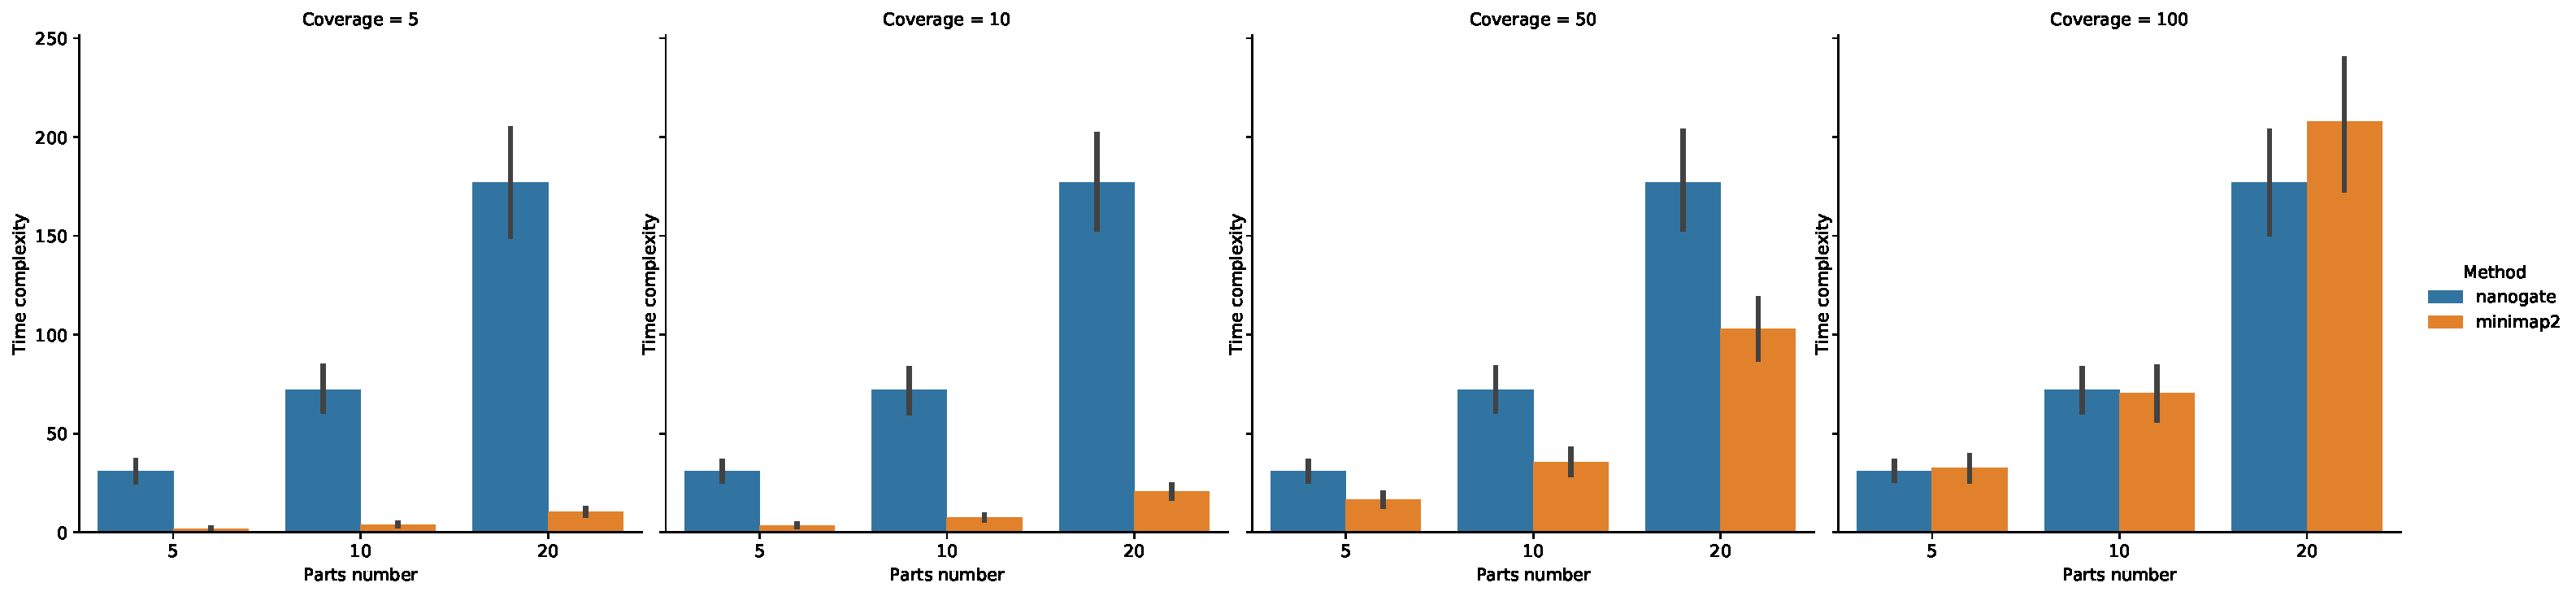
\includegraphics[width=1.35\textwidth]{../results/images_notebook/v_400/sim_09_minimap2_nanogate_time_comparison.pdf}
    \end{center}
    \caption{{\bf Nanogate and Minimap2 time comparison plot.} This plot shows, for parts similarity$=90\%$, the time complexity comparison between Nanogate and Minimap2 using as query only constructs reads.}
   \label{fig:v_400_sim_09_time_comparison}
\end{figure}
 
  \begin{figure}[ht]
    \begin{center}
    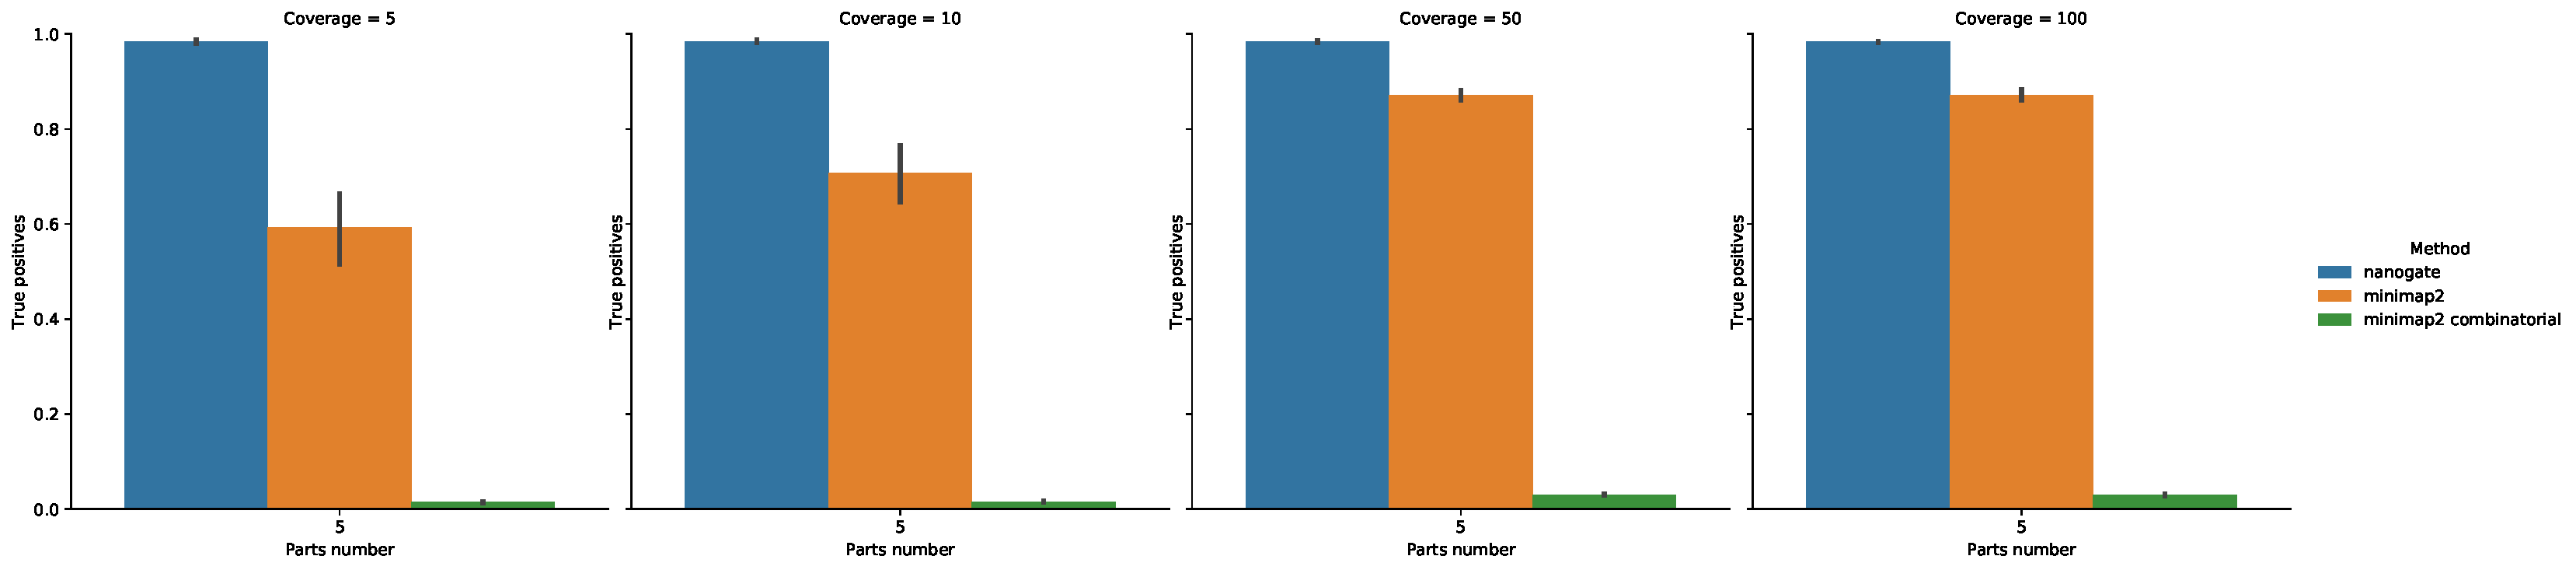
\includegraphics[width=1.35\textwidth]{../results/images_notebook/v_400/sim_00_5_parts_true_positives_comparison.pdf}
    \end{center}
    \caption{{\bf Nanogate Minimap2 and combinatorial assembly true positives.}  This plot shows, in absence of parts similarity, the true positives comparison between Nanogate, Minimap2 using as query only constructs reads, and Minimap2 applied to combinatorial assemblies. To simplify the analysis only 5 parts constructs are taken into account.}
   \label{fig:v_400_sim_00_5_parts_true_positives_comparison}
\end{figure}

  \begin{figure}[ht]
    \begin{center}
    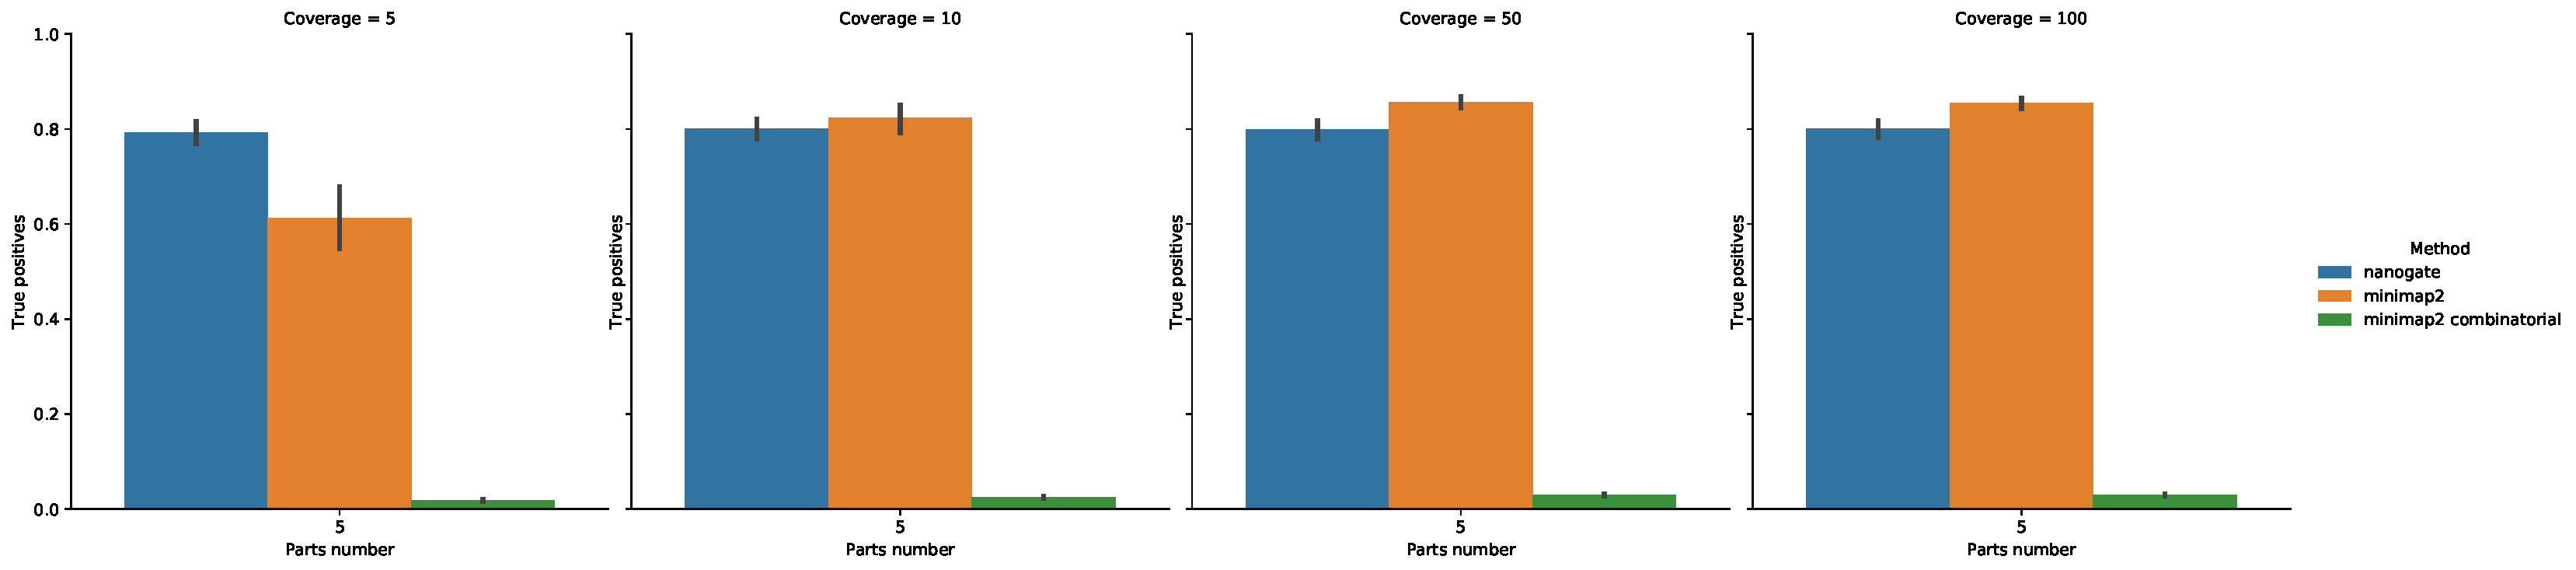
\includegraphics[width=1.35\textwidth]{../results/images_notebook/v_400/sim_09_5_parts_true_positives_comparison.pdf}
    \end{center}
    \caption{{\bf Nanogate Minimap2 and combinatorial assembly true positives.}  This plot shows, for parts similarity $=90\%$, the true positives comparison between Nanogate, Minimap2 using as query only constructs reads, and Minimap2 applied to combinatorial assemblies. To simplify the analysis only 5 parts constructs are taken into account.}
   \label{fig:v_400_sim_90_5_parts_true_positives_comparison}
\end{figure}

  \begin{figure}[ht]
    \begin{center}
    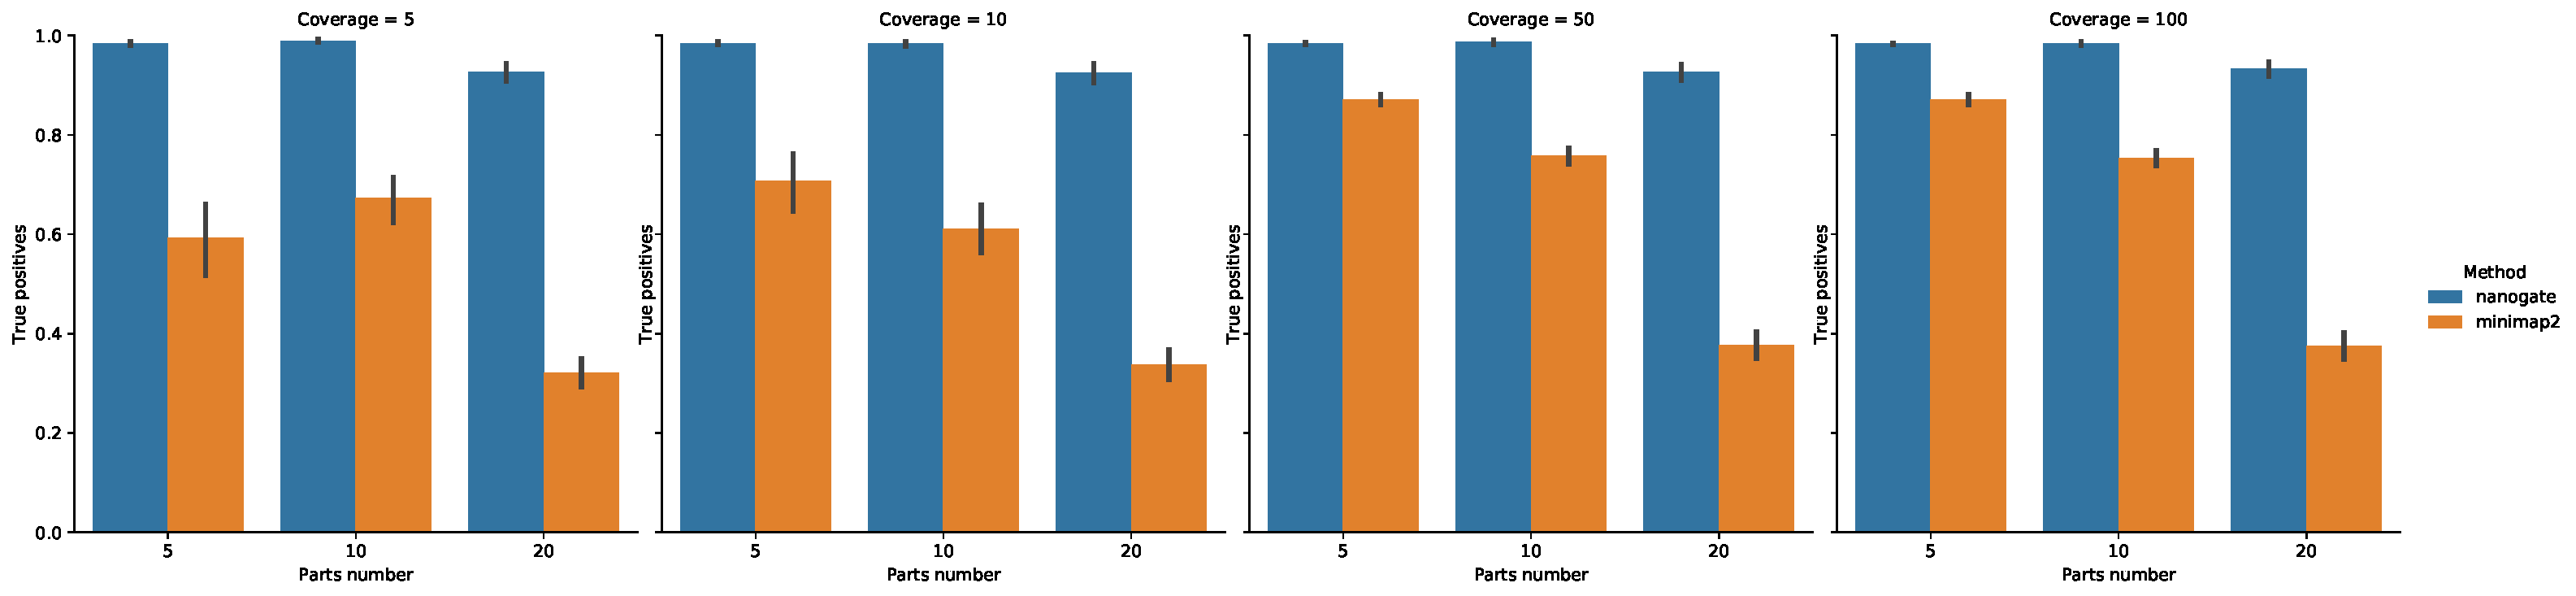
\includegraphics[width=1.35\textwidth]{../results/images_notebook/v_400/sim_00_minimap2_nanogate_true_positives_comparison.pdf}
    \end{center}
    \caption{{\bf Nanogate Minimap2 true positives.}  This plot shows, in absence of parts similarity, the true positives comparison between Nanogate and Minimap2 using as query only constructs reads.}
   \label{fig:v_400_sim_00_true_positives_comparison}
\end{figure}

  \begin{figure}[ht]
    \begin{center}
    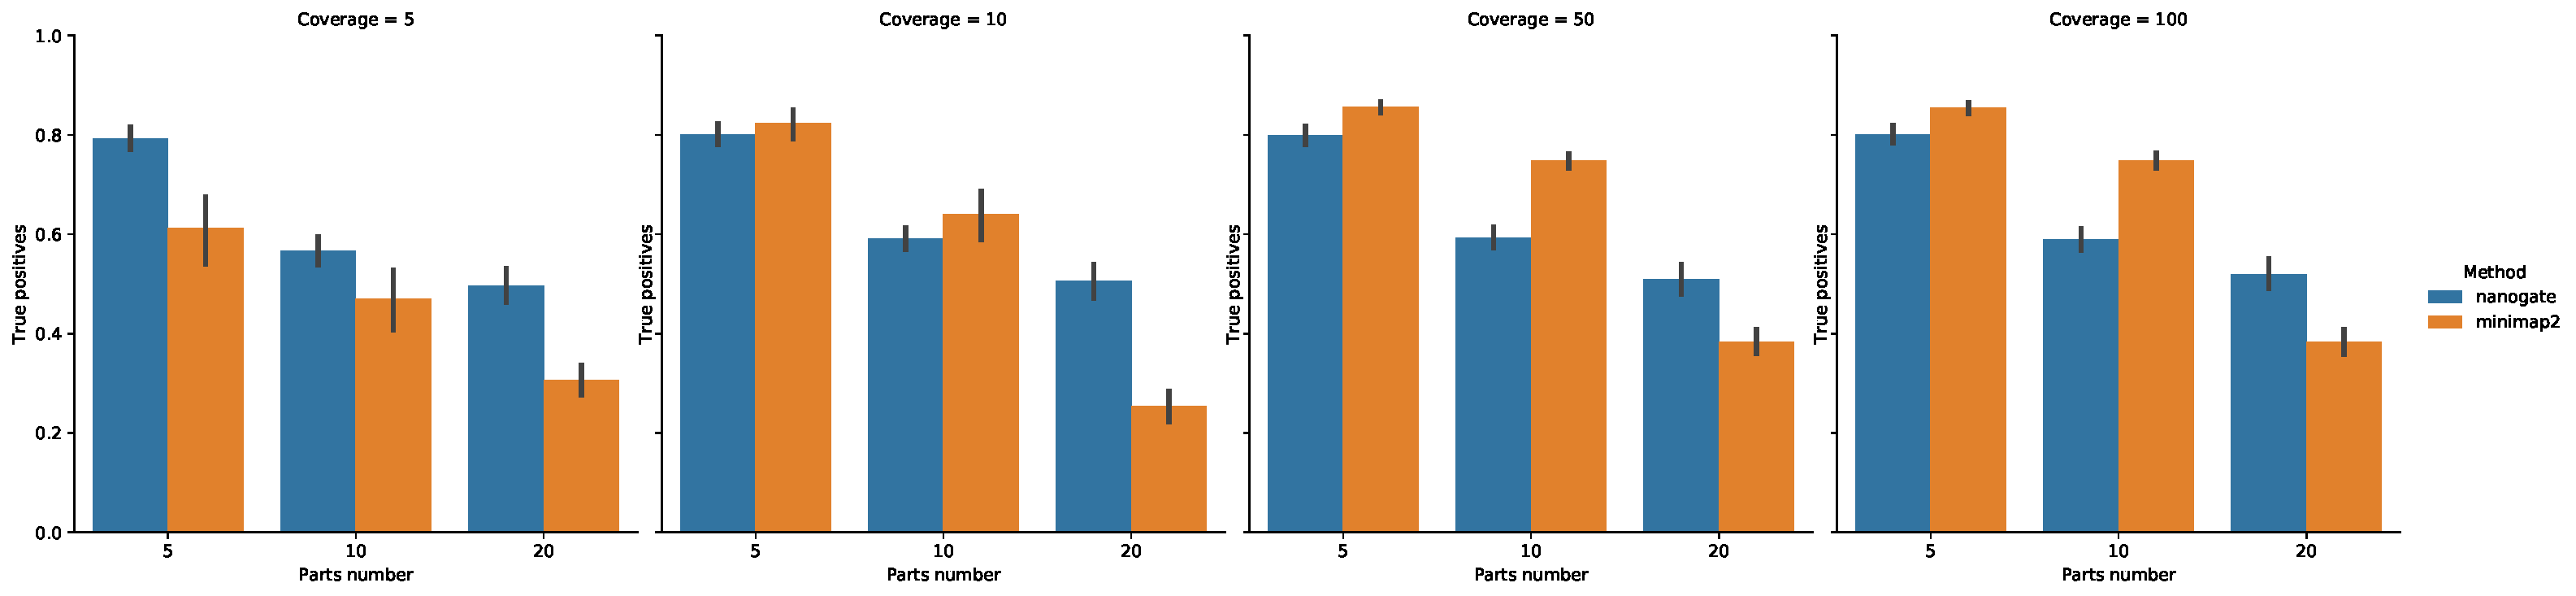
\includegraphics[width=1.35\textwidth]{../results/images_notebook/v_400/sim_09_minimap2_nanogate_true_positives_comparison.pdf}
    \end{center}
    \caption{{\bf Nanogate Minimap2 true positives.}  This plot shows, for parts similarity$=90\%$, the true positives comparison between Nanogate and Minimap2 using as query only constructs reads.}
   \label{fig:v_400_sim_90_true_positives_comparison}
\end{figure}

\clearpage
\subsection{V4.5.0 }
Results in this section can be obtained by running the following pipeline:
\begin{lstlisting}[language=Python]
    project: "bad_reads_sim_00"
    genbank: "yeast_chromosome_xiv.gb"
    run: 10
    
    generate_testbeds:
        cds_number : 50
        constructs_number: [10,50,100]
        parts : [5,10,20]
        constructs_similarity : 0.0
        parts_similarity : 0.0
        mutation_method : "last"
    
    badreads:
        quantity : [5x,10x,50x,100x]
        error_model: "nanopore"
        qscore_model: "nanopore"
        glitches: "1000,100,100"
        junk_reads: 5
        random_reads: 5
        chimeras: 10
        identity: 75,90,8
        start_adapter_seq: ' "" '
        end_adapter_seq: ' "" '
    
    combinatorial_assembly:
        max_parts: 5
    
    nanogate:
        error_rate : ["001","010","030"]
        jaccard_thresholds: ["00","002","004","006","007","008","01"]

\end{lstlisting}

 \begin{figure}[ht]
    \begin{center}
    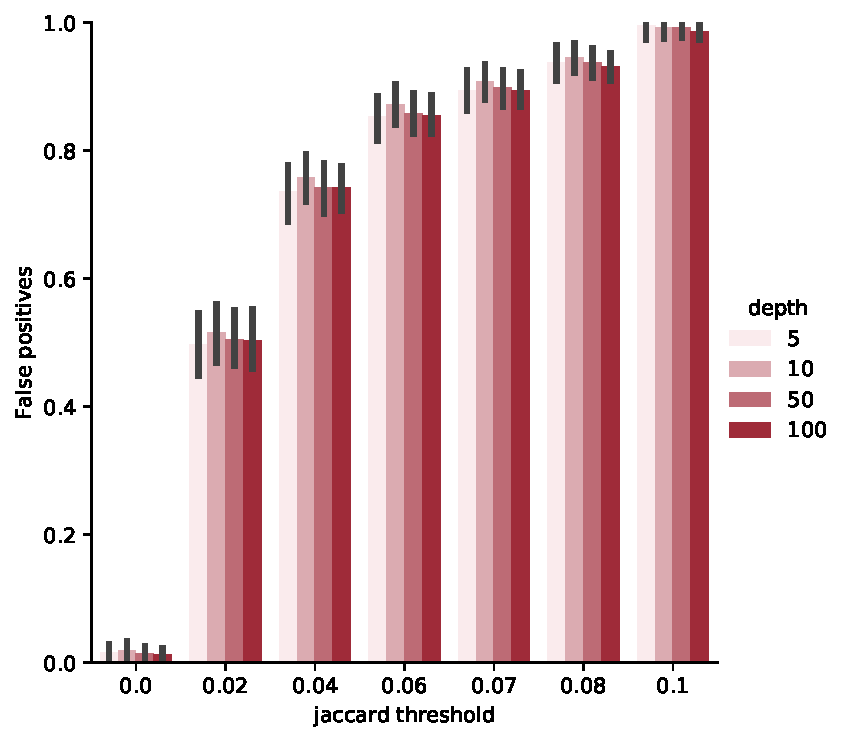
\includegraphics[width=1.35\textwidth]{../results/images_notebook/v_450/sim_00_false_positive.pdf}
    \end{center}
    \caption{{\bf Nanogate true positives.}  This plot shows, in absence of parts similarity, the false positives rate. To evaluate false positives only junk reads and random reads are taken into consideration. A false positive is evaluated as the ratio 
    $p_0/br$, where $p_0$ is number of junk or random reads with no part assigned and $br$ is the number of the overall number of junk and random reads}
   \label{fig:v_450_sim_00_false_positives}
\end{figure}

 \begin{figure}[ht]
    \begin{center}
    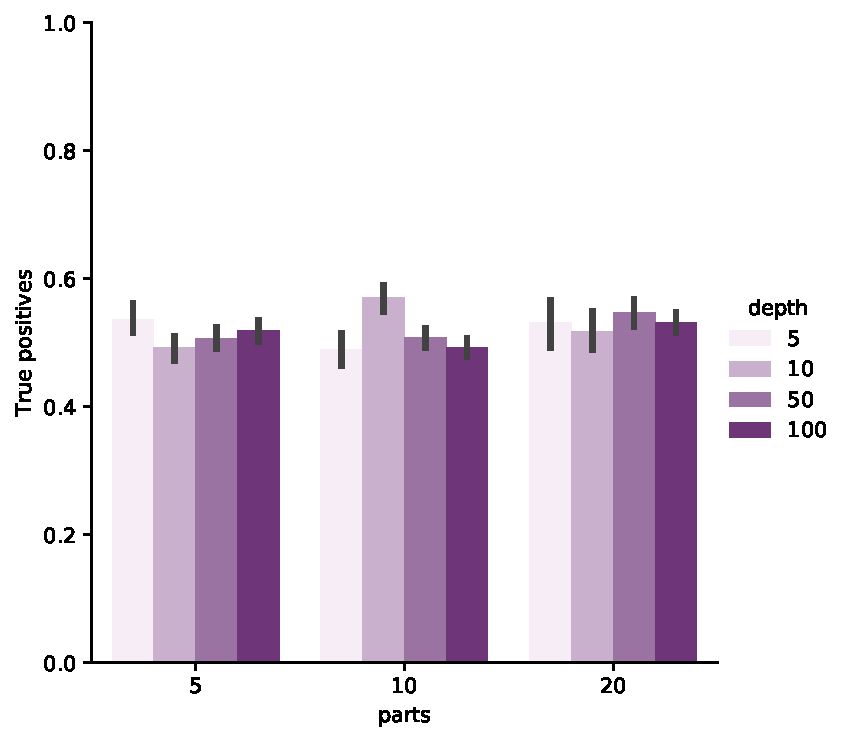
\includegraphics[width=1.35\textwidth]{../results/images_notebook/v_450/sim_00_good_reads_true_positves.pdf}
    \end{center}
    \caption{{\bf Nanogate true positives.}  This plot shows, in absence of parts similarity, the true positives rate when Nanogate is applied to reads with a bad quality }
   \label{fig:v_450_sim_00_good_read_true_positives}
\end{figure}

 \begin{figure}[ht]
    \begin{center}
    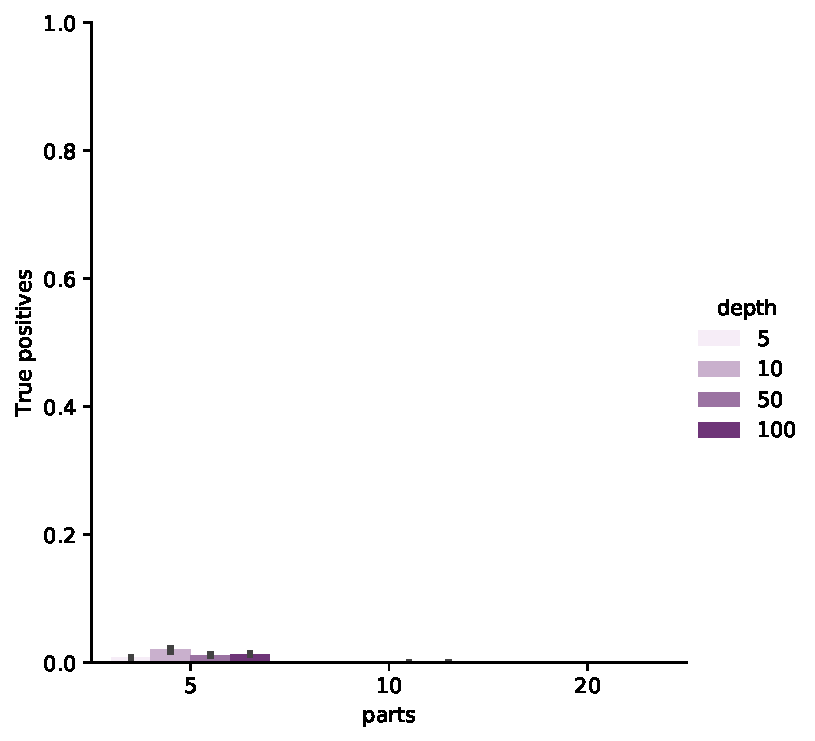
\includegraphics[width=1.35\textwidth]{../results/images_notebook/v_450/sim_90_good_reads_true_positves.pdf}
    \end{center}
    \caption{{\bf Nanogate true positives.}  This plot shows the true positives rate when Nanogate is applied to reads with a bad quality and the parts similarity $=90\%$ }
   \label{fig:v_450_sim_90_true_positives}
\end{figure}


 \begin{figure}[ht]
    \begin{center}
    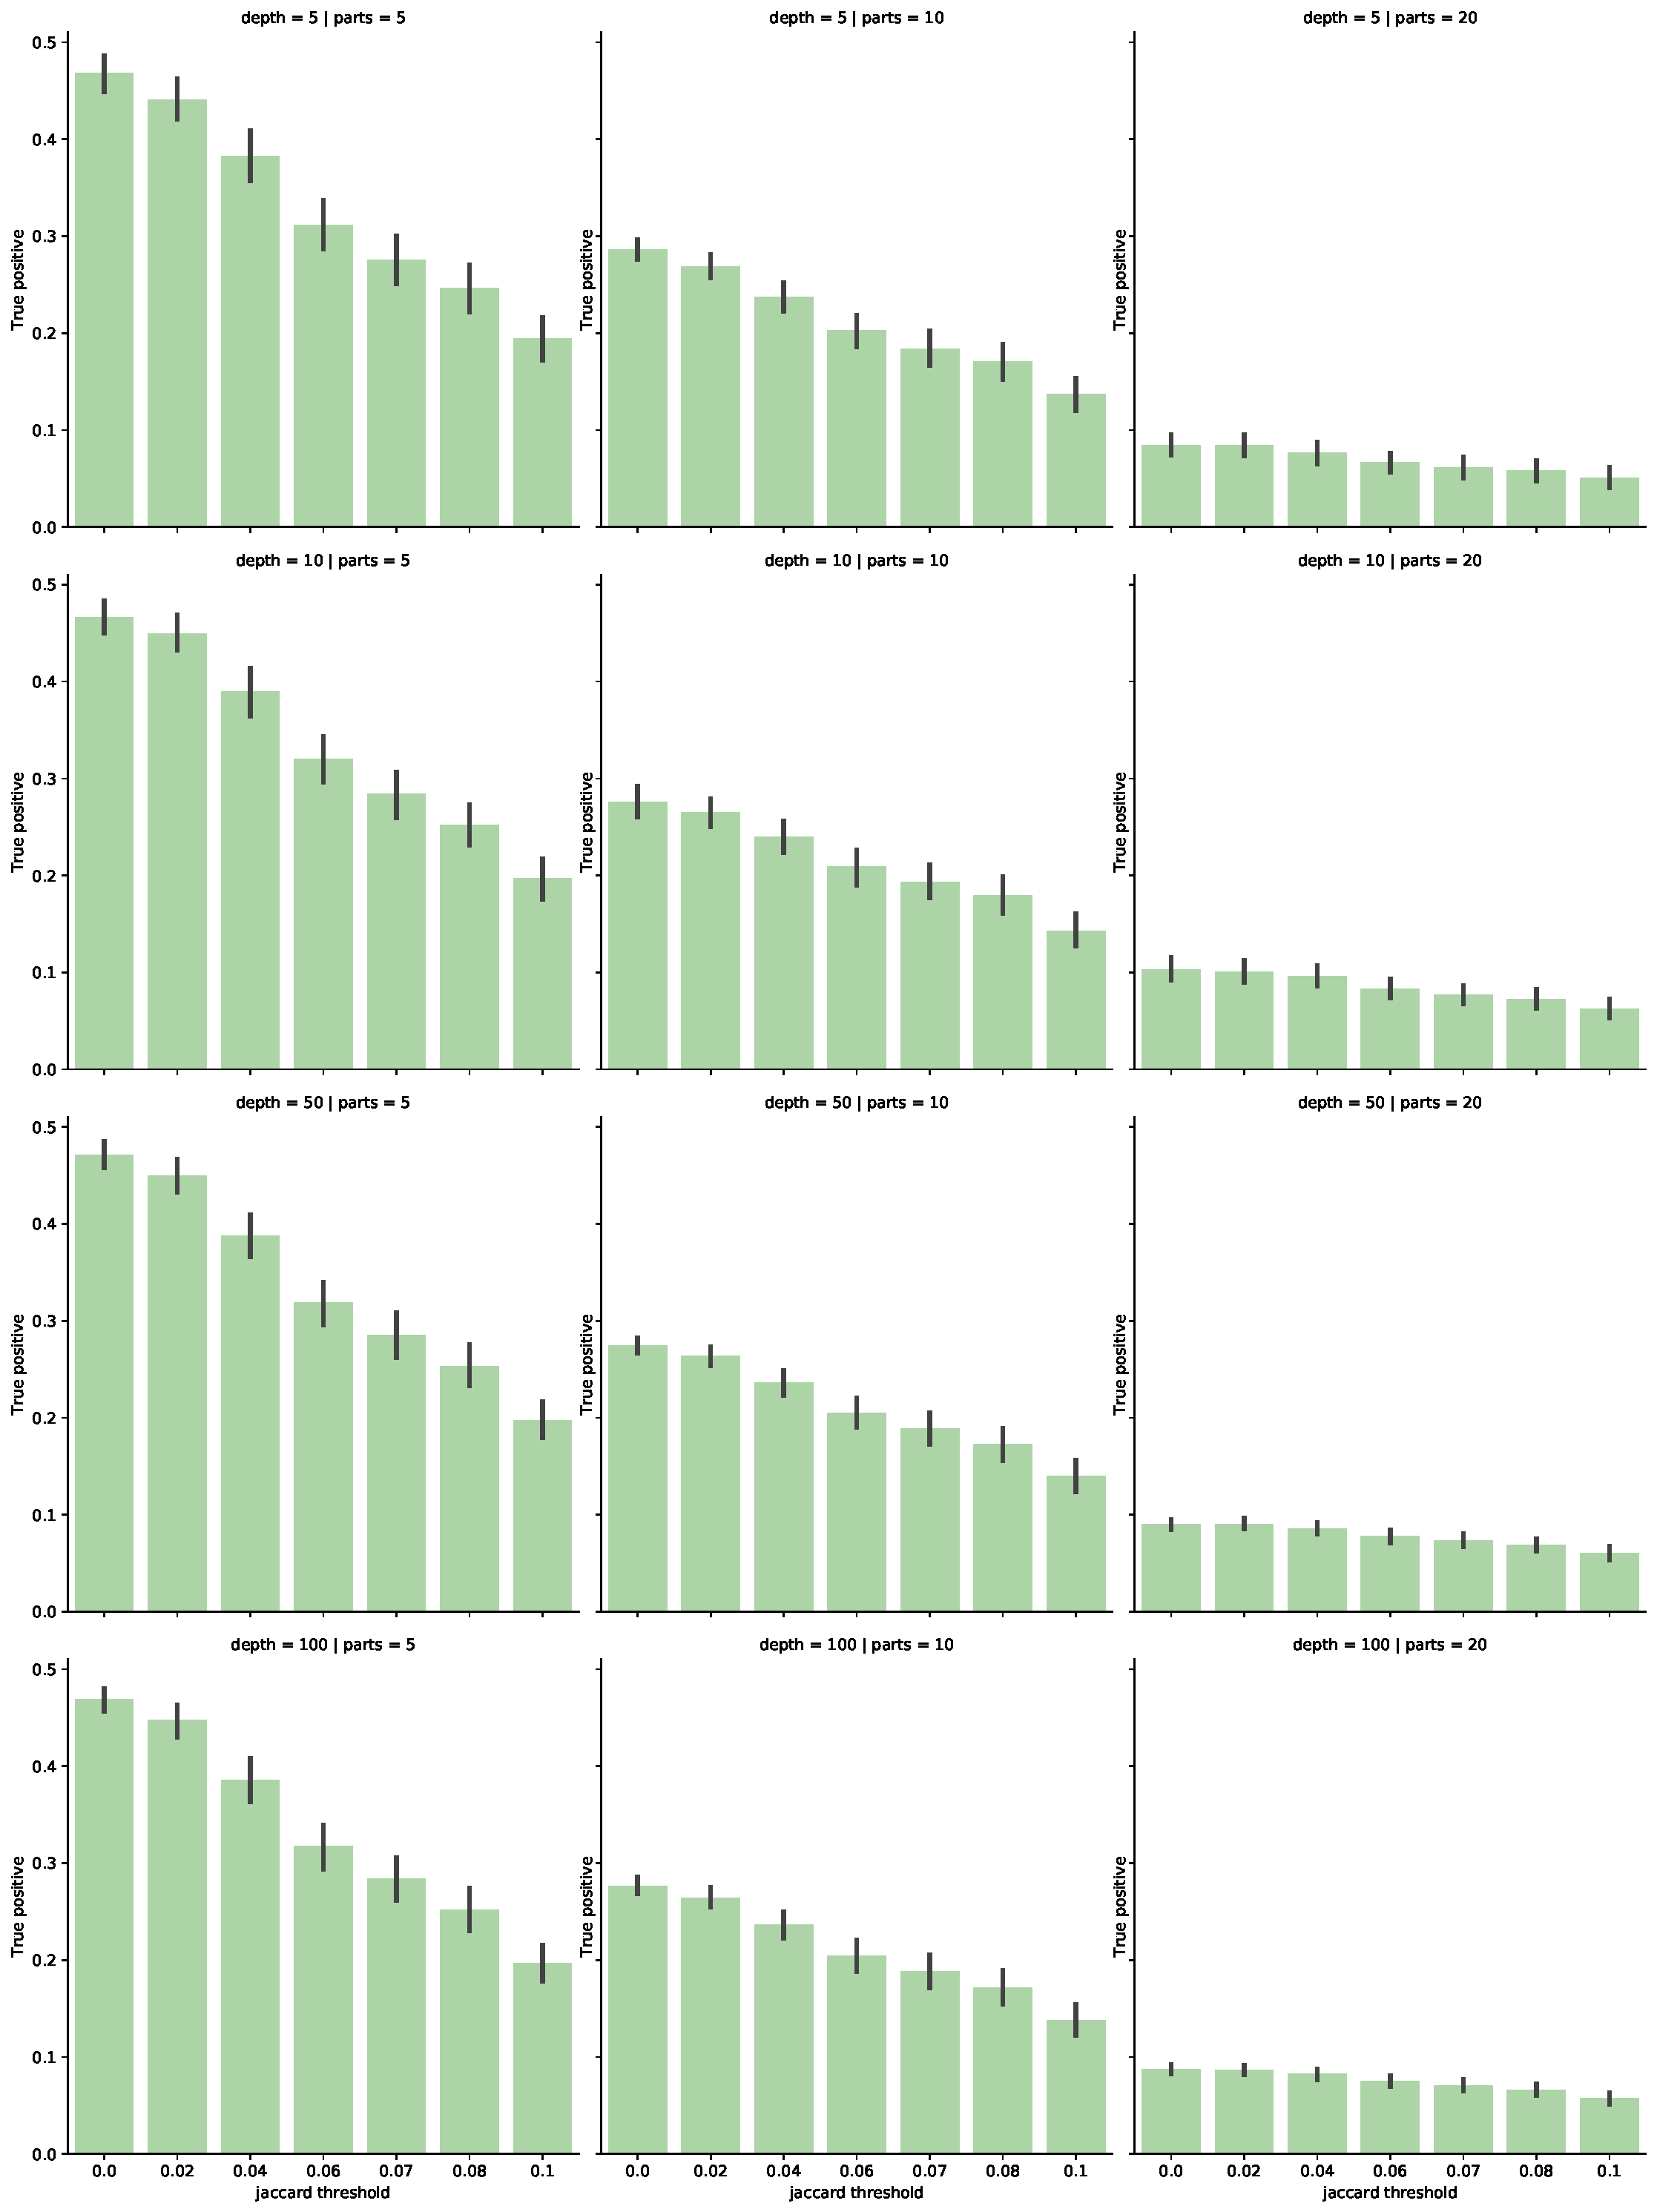
\includegraphics[width=1.35\textwidth]{../results/images_notebook/v_450/sim_00_true_positive.pdf}
    \end{center}
    \caption{{\bf Nanogate true positives.}  This plot shows, in absence of parts similarity, the true positives rate when Nanogate is applied to reads with a bad quality.Here all reads who pass the Nanogate filter are considered not only those with a length $>= 99\%$ of the original construct length . }
   \label{fig:v_450_sim_00_true_positives}
\end{figure}


 \begin{figure}[ht]
    \begin{center}
    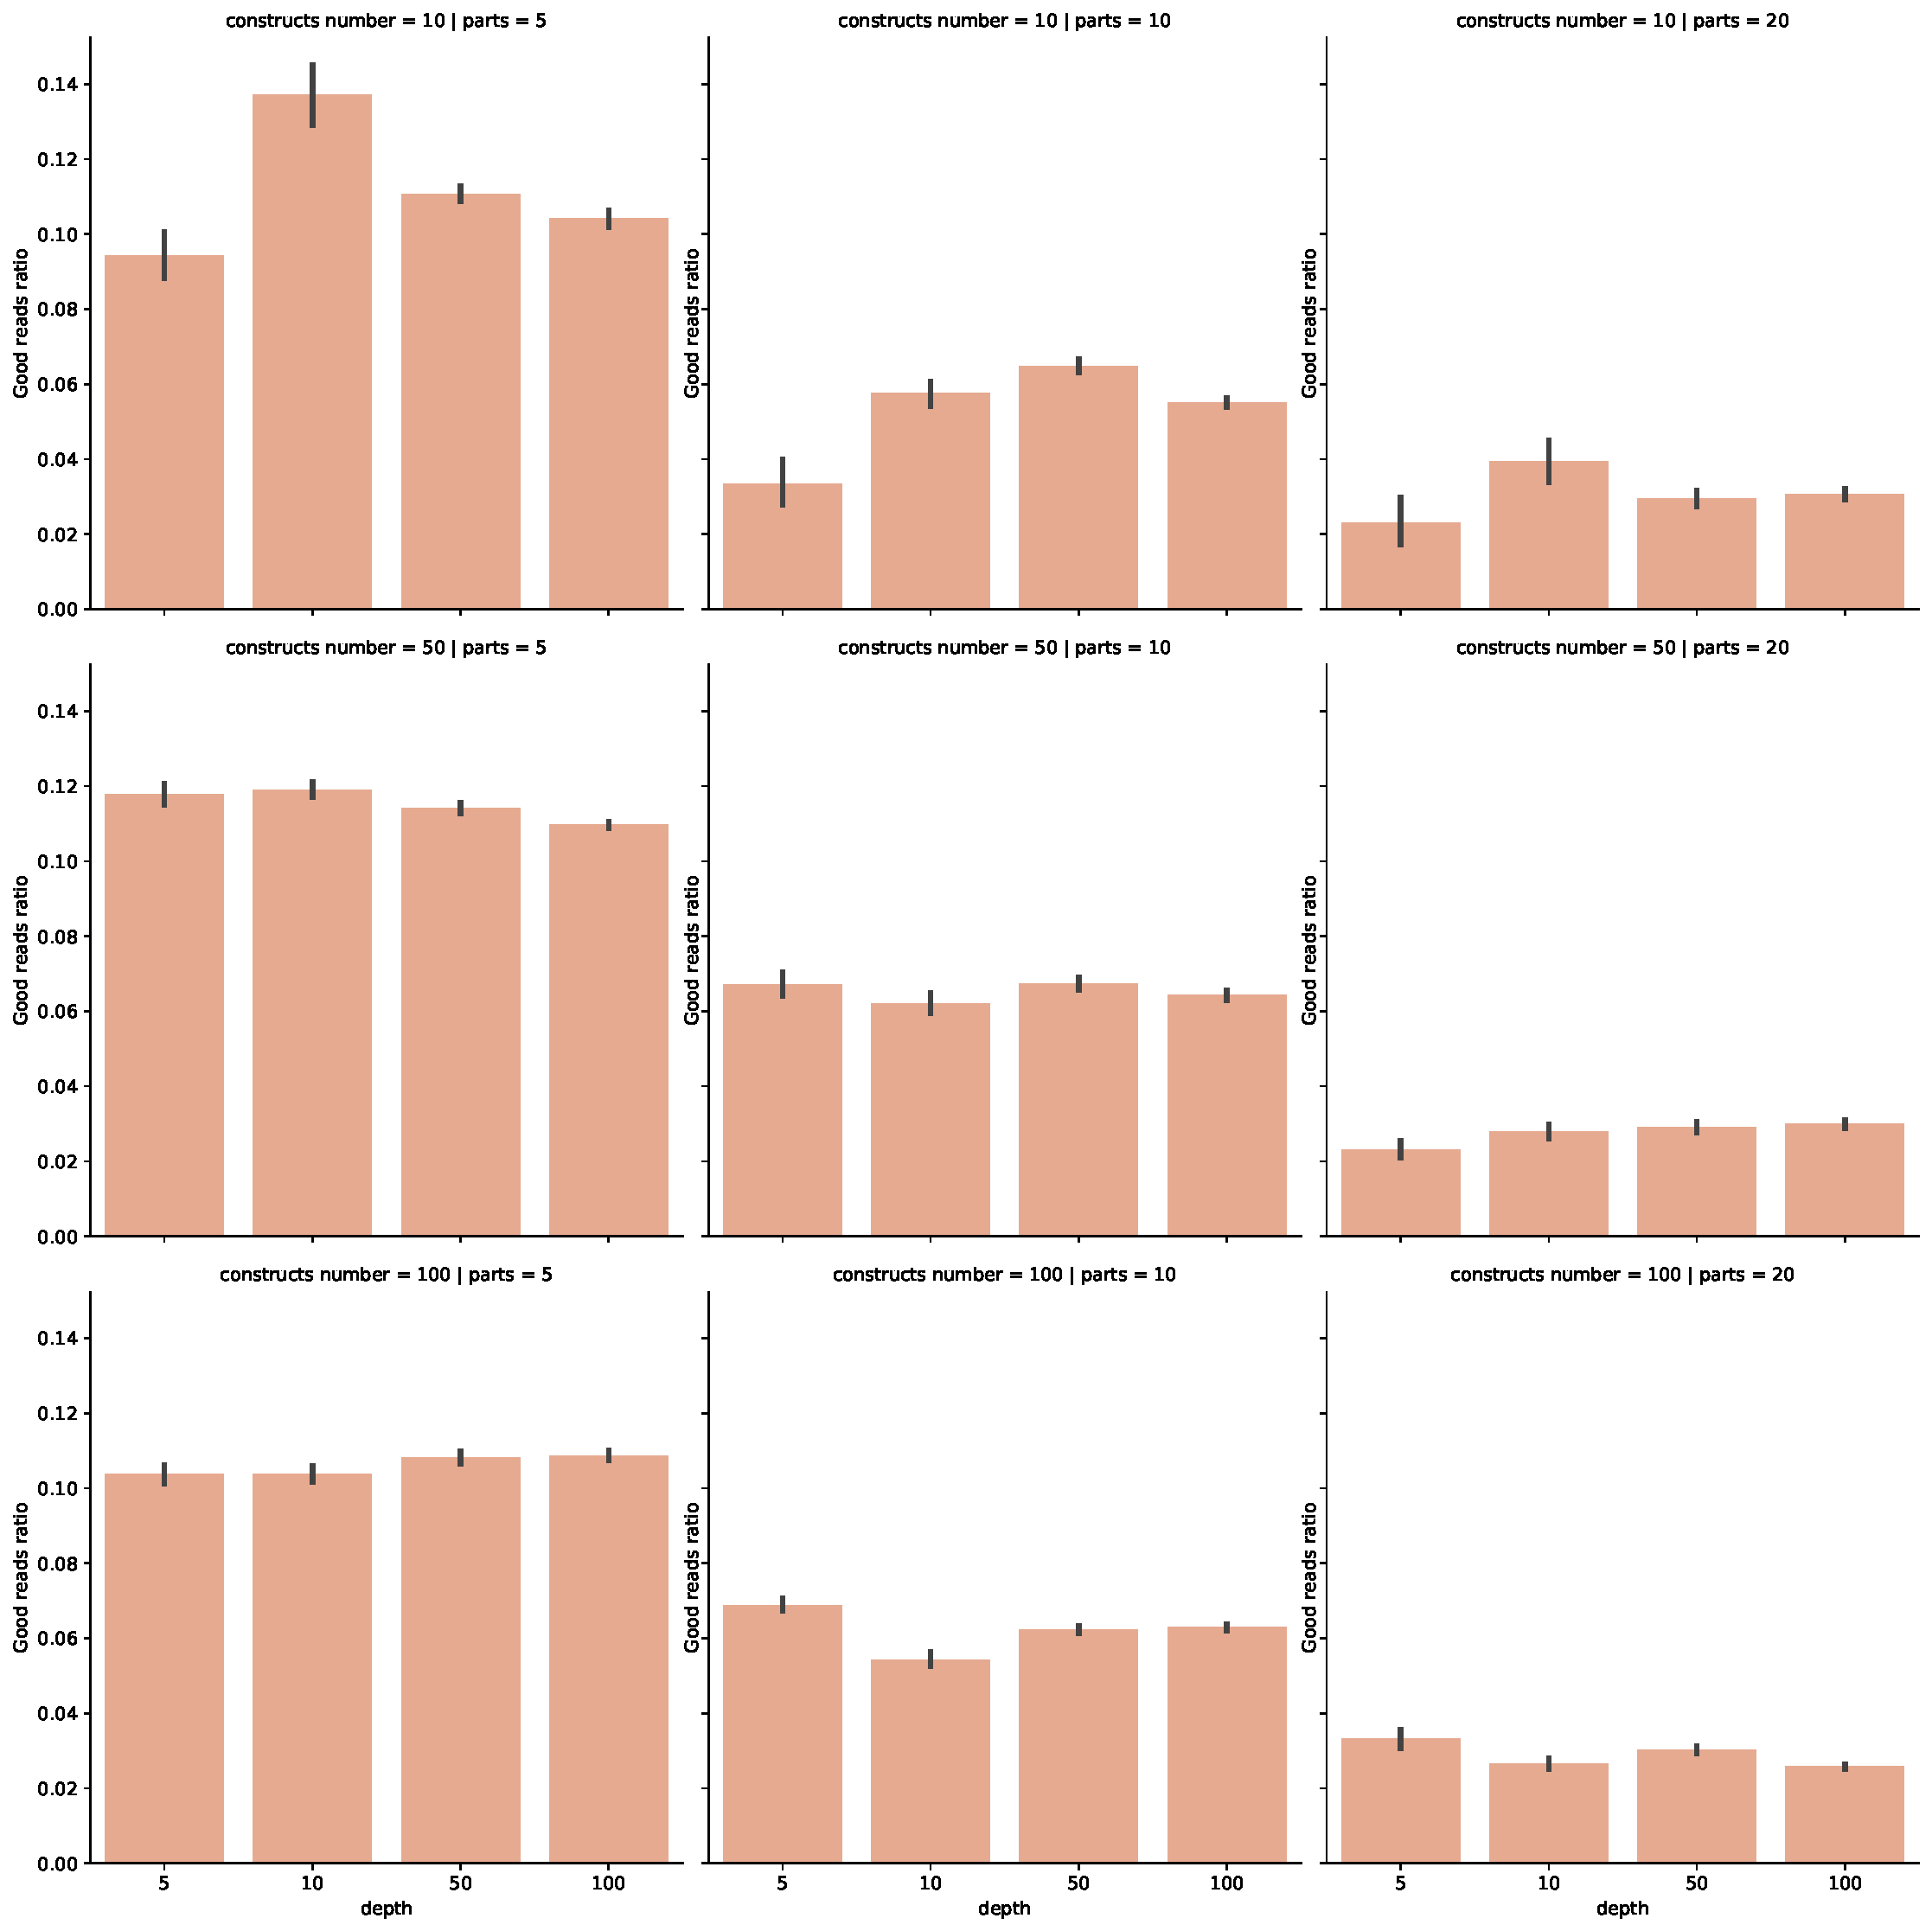
\includegraphics[width=1.35\textwidth]{../results/images_notebook/v_450/sim_00_good_reads_ratio.pdf}
    \end{center}
    \caption{{\bf Reads quality.}  This plot shows the ratio $99r/r$, where $99r$ is the amount read with a length $>=99\%$ of the original construct length, and $r$ is the amount of all read analysed}
   \label{fig:v_450_good_reads_ratio}
\end{figure}

 \begin{figure}[ht]
    \begin{center}
    \includegraphics[width=1.35\textwidth]{../results/images_notebook/v_450/sim_00_mismatch_per_error.pdf}
    \end{center}
    \caption{{\bf Mismatch error.}  This plot shows the ratio $m/e$, where $m$ is amount of reads including at least of mismatch and $e$ is the amount of reads analysed incorrectly. This plot shows how much of the Nanogate error is due to a part assigned incorrectly.}
   \label{fig:v_450_mismatch_error }
\end{figure}

 \begin{figure}[ht]
    \begin{center}
    \includegraphics[width=1.35\textwidth]{../results/images_notebook/v_450/sim_00_short_reads_per_error.pdf}
    \end{center}
    \caption{{\bf Reads error.}  This plot shows the ratio $er/e$, where $er$ is the amount of reads including a different number of parts compared to the construct from which they derived.$e$ is the amount of reads analysed incorrectly. These plot shows how much of the error is due to reads longer or shorter than the original construct, and as consequence they include more or less parts}
   \label{fig:v_450_parts_error }
\end{figure}

 \begin{figure}[ht]
    \begin{center}
    \includegraphics[width=1.35\textwidth]{../results/images_notebook/v_450/sim_00_parts_positive.pdf}
    \end{center}
    \caption{{\bf Parts true positives.}  This plot shows the ratio $pc/p$, where $pc$ is the amount of parts correctly called and $p$ is the amount of all parts analysed.This plot show how many parts have been assigned correctly.The similarity between parts $=0\%$ in this plot}
   \label{fig:v_sim_00_450_parts_positives }
\end{figure}

 \begin{figure}[ht]
    \begin{center}
    \includegraphics[width=1.35\textwidth]{../results/images_notebook/v_450/sim_90_parts_positive.pdf}
    \end{center}
    \caption{{\bf Parts true positives.}  This plot shows the ratio $pc/p$, where $pc$ is the amount of parts correctly called and $p$ is the amount of all parts analysed.This plot show how many parts have been assigned correctly.The similarity between parts $=90\%$ in this plot}
   \label{fig:v_450_sim_90_parts_positives }
\end{figure}
\clearpage
\subsection{V4.6.0 }
\begin{lstlisting}[language=Python]
    project: "bad_reads_sim_00"
    genbank: "yeast_chromosome_xiv.gb"
    run: 10
    
    generate_testbeds:
        cds_number : 50
        constructs_number: [10,50,100]
        parts : [5,10,20]
        constructs_similarity : 0.0
        parts_similarity : 0.0
        mutation_method : "last"
    
    badreads:
        quantity : [5x,10x,50x,100x]
        error_model: "nanopore"
        qscore_model: "nanopore"
        glitches: "1000,100,100"
        junk_reads: 5
        random_reads: 5
        chimeras: 10
        identity: 75,90,8
        start_adapter_seq: ' "" '
        end_adapter_seq: ' "" '
    
    combinatorial_assembly:
        max_parts: 5
    
    nanogate:
        error_rate : ["001","010","030"]
        jaccard_thresholds: ["00","002","004","006","007","008","01"]

\end{lstlisting}

\subsubsection{Contaminant discovery}
Random and junk reads are analysed separately from others, here I show the ratio
\begin{equation}
    cd = \mbox{contaminants detected}/ \mbox{all contaminants}
\end{equation}

 \begin{figure}[ht]
    \begin{center}
    \includegraphics[width=1.35\textwidth]{../results/images_notebook/v_460/lq_sim_70_contaminant_discovery.pdf}
    \end{center}
    \caption{{\bf Contaminants discovery.}  This plot shows the ratio between the detected contaminants and all contaminants.We see how increasing the $J_t$, the contaminant discovery increase as well. Contaminants discovery is applied only on low quality reads, here in particular  }
   \label{fig:v_460_sim_70_contaminant_discovery}
\end{figure}
\clearpage
\subsubsection{Reads quality analysis}
In this version of Nanogate we are analysing only pass reads. We mark reads as pass, if Nanogate assign them the preset number of parts. Here I show the difference in terms of reads analysed between the high quality setting and the low quality.

 \begin{figure}[ht]
    \begin{center}
    \includegraphics[width=1.35\textwidth]{../results/images_notebook/v_460/hq_sim_00_good_reads_ratio.pdf}
    \end{center}
    \caption{{\bf High quality reads analysed .}  This plot show ration of reads analysed who passed the Nanogate filter, here I measure the ratio between reads who passed the filter and are marked as pass and every reads who pass the filter. The analysis is performed on High quality reads and in absence of parts similarity.}
   \label{fig:v_460_sim_00_hq_reads_quality}
\end{figure}

 \begin{figure}[ht]
    \begin{center}
    \includegraphics[width=1.35\textwidth]{../results/images_notebook/v_460/lq_sim_90_good_reads_ratio.pdf}
    \end{center}
    \caption{{\bf Low quality reads analysed .}  This plot show ration of reads analysed who passed the Nanogate filter, here I measure the ratio between reads who passed the filter and are marked as pass and every reads who pass the filter. The analysis is performed on Low quality reads and with parts similarity $= 90\%$.}
   \label{fig:v_460_sim_90_reads_quality}
\end{figure}
\clearpage
\subsubsection{Confusion matrix analysis}
Here I analyse Nanogate precision and recall. \\
Positivity definition:
\begin{itemize}
    \item \textbf{True Positive(TP)} read correctly analysed by Nanogate, where all parts are predicted correctly
      \item \textbf{False Positive(FP)} read analysed incorrectly, which composition defined by Nanogate matches the composition of another construct in the pool
    \item \textbf{False Negative(FN)} read analysed incorrectly, which composition defined by Nanogate matches none of the construct in the pool
\end{itemize}


\begin{equation}
    Recall = \frac{TP}{TP + FN}
\end{equation}

      
\begin{equation}
    Precision = \frac{TP}{TP + FP}
\end{equation}


 \begin{figure}[ht]
    \begin{center}
    \includegraphics[width=1.35\textwidth]{../results/images_notebook/v_460/hq_sim_00_recall_per_result.pdf}
    \end{center}
    \caption{{\bf High quality recall per result .}  This plot shows the recall related to the high quality setting, in absence of parts similarity. The recall is evaluated on each each Nanogate output, each point represent the recall evaluated on a single output}
   \label{fig:v_460_hq_sim_00_recall_per_result}
\end{figure}

 \begin{figure}[ht]
    \begin{center}
    \includegraphics[width=1.35\textwidth]{../results/images_notebook/v_460/lq_sim_00_recall_per_result.pdf}
    \end{center}
    \caption{{\bf Low quality recall per result similarity $0\%$ .}  This plot shows the recall related to the low quality setting, in absence of parts similarity. The recall is evaluated on each each Nanogate output, each point represent the recall evaluated on a single output}
   \label{fig:v_460_lq_sim_00_recall_per_result}
\end{figure}


 \begin{figure}[ht]
    \begin{center}
    \includegraphics[width=1.35\textwidth]{../results/images_notebook/v_460/lq_sim_00_recall_per_construct.pdf}
    \end{center}
    \caption{{\bf Low quality recall per construct similarity $0\%$ .}  This plot shows the recall related to the low quality setting, in absence of parts similarity. The recall is evaluated on each construct, each point represent a construct}
   \label{fig:v_460_lq_sim_00_recall_per_construct}
\end{figure}


 \begin{figure}[ht]
    \begin{center}
    \includegraphics[width=1.35\textwidth]{../results/images_notebook/v_460/lq_sim_90_recall_per_result.pdf}
    \end{center}
    \caption{{\bf Low quality recall per result similarity $90\%$ .}  This plot shows the recall related to the low quality setting, with parts similarity $=90\%$. The recall is evaluated on each each Nanogate output, each point represent the recall evaluated on a single output}
   \label{fig:v_460_lq_sim_90_recall_per_result}
\end{figure}

 \begin{figure}[ht]
    \begin{center}
    \includegraphics[width=1.35\textwidth]{../results/images_notebook/v_460/lq_sim_90_recall_per_construct.pdf}
    \end{center}
    \caption{{\bf Low quality recall per construct similarity $90\%$ .}  This plot shows the recall related to the low quality setting, with parts similarity $=90\%$. The recall is evaluated on each construct, each point represent a construct}
   \label{fig:v_460_lq_sim_90_recall_per_construct}
\end{figure}


 \begin{figure}[ht]
    \begin{center}
    \includegraphics[width=1.35\textwidth]{../results/images_notebook/v_460/hq_sim_00_precision_per_result.pdf}
    \end{center}
    \caption{{\bf High quality precision per result similarity $0\%$ .}  This plot shows the precision related to the high quality setting, with parts similarity $=0\%$. The precision is evaluated on each each Nanogate output, each point represent the recall evaluated on a single output. (The plot is correct, there is a bug with labels, this plot shows the precision)}
   \label{fig:v_460_hq_sim_00_precision_per_result}
\end{figure}


 \begin{figure}[ht]
    \begin{center}
    \includegraphics[width=1.35\textwidth]{../results/images_notebook/v_460/lq_sim_00_precision_per_result.pdf}
    \end{center}
    \caption{{\bf Low quality precision per result similarity $0\%$ .}  This plot shows the precision related to the low quality setting, with parts similarity $=0\%$. The precision is evaluated on each each Nanogate output, each point represent the recall evaluated on a single output. (The plot is correct, there is a bug with labels, this plot shows the precision)}
   \label{fig:v_460_lq_sim_00_precision_per_result}
\end{figure}

 \begin{figure}[ht]
    \begin{center}
    \includegraphics[width=1.35\textwidth]{../results/images_notebook/v_460/lq_sim_00_precision_per_construct.pdf}
    \end{center}
    \caption{{\bf Low quality precision per construct similarity $0\%$ .}  This plot shows the precision related to the low quality setting, with parts similarity $=0\%$. The precision is evaluated on each construct, each point represent a construct. (The plot is correct, there is a bug with labels, this plot shows the precision)}
   \label{fig:v_460_lq_sim_00_precision_per_construct}
\end{figure}


 \begin{figure}[ht]
    \begin{center}
    \includegraphics[width=1.35\textwidth]{../results/images_notebook/v_460/lq_sim_90_recall_per_result.pdf}
    \end{center}
    \caption{{\bf Low quality precision per construct similarity $90\%$ .}  This plot shows the precision related to the low quality setting, with parts similarity $=90\%$. The precision is evaluated on each each Nanogate output, each point represent the precision evaluated on a single output. (The plot is correct, there is a bug with labels, this plot shows the precision)}
   \label{fig:v_460_lq_sim_90_precision_per_result}
\end{figure}

\clearpage
\subsection{Latest version V5.0.0 }
In this section I am showing for the first time results related to the parts order.

\subsubsection{High quality reads analysis}
\paragraph{Reads quality analysis}
The following plot shows the ratio between the reads who passed the Nanogate filter and the the reads marked as pass.
The reads marked as pass are all the reads to which Nanogate assigned the correct number of parts, as consequence these reads are long enough to include a number of parts equal to the number of parts in the original construct.

\begin{equation}
        \text{Parts analysed} = \text{pass reads}/ \text{total reads}
\end{equation}


 \begin{figure}[ht]
    \begin{center}
    \includegraphics[width=1.35\textwidth]{../results/images_notebook/v_500/hq_sim_00_good_reads_ratio.pdf}
    \end{center}
    \caption{{\bf High quality reads analysis.}  This plot shows the percentage of reads analysed in relation to the depth and number of parts.The number of parts is the main factor affecting the number of reads analysed followed to the depth. The reads analysed are high quality and there is no similarity between parts.}
   \label{fig:v_500_hq_sim_00_good_reads_ratio}
\end{figure}


 \begin{figure}[ht]
    \begin{center}
    \includegraphics[width=1.35\textwidth]{../results/images_notebook/v_500/lq_sim_00_good_reads_ratio.pdf}
    \end{center}
    \caption{{\bf Low quality reads analysis.}  This plot shows the percentage of reads analysed in relation to the depth and number of parts.The number of parts is the main factor affecting the number of reads analysed followed to the depth. The reads analysed are low quality and there is no similarity between parts.For the low quality setting the percentage of the reads analysed is at maximum $40\%$ for constructs with $5$ parts, half of the high quality setting. The minimum is instead $10\%$.For the low quality setting the percentage decrease linearly with the the number of parts per construct.}
   \label{fig:v_500_lq_sim_00_good_reads_ratio}
\end{figure}

 \begin{figure}[ht]
    \begin{center}
    \includegraphics[width=1.35\textwidth]{../results/images_notebook/v_500/hq_sim_00_10_reads_constructs.pdf}
    \end{center}
    \caption{{\bf High quality constructs with at least $10$ reads.} Here I show the amount of constructs with more than $10$
reads.In this plot is clear how the depths 5x and 10x generate a low amount of reads, in particular for 10 and 20 parts constructs there is almost no construct with more than 10 reads. The number of reads per constructs is affected by the depth, the size of the constructs library and the number of parts per constructs.     
The reads analysed are high quality and there is no similarity between parts}
   \label{fig:v_500_hq_sim_00_10_reads_construct}
\end{figure}


\begin{figure}[ht]
    \begin{center}
    \includegraphics[width=1.35\textwidth]{../results/images_notebook/v_500/lq_sim_00_10_reads_constructs.pdf}
    \end{center}
    \caption{{\bf Low quality constructs with at least $10$ reads.} Here I show the amount of constructs with more than $10$
reads.In this plot is clear how the depths 5x and 10x generate a low amount of reads. Indeed, for $5x$ and $10x$ depths there is no construct with more than 10 reads. For construct with 20 parts none of the depths generates constructs with more than 10 reads 
The number of reads per constructs is affected by the depth, the size of the constructs library and the number of parts per constructs.     
The reads analysed are low quality and there is no similarity between parts}
   \label{fig:v_500_lq_sim_00_10_reads_construct}
\end{figure}

\clearpage
\subsubsection{Nanogate qualitative analysis }
Here I show plots related to the qualitative analysis of Nanogate taking into account results related only the parts present or absent in construct. I do not take into account the parts order.
In particular I am analysing the precision
\begin{equation}
    Precision = \frac{TP}{TP + FP}
\end{equation}

$TP$ = Nanogate predicted correctly every part in the construct
$FP$ = Nanogate did not predict correctly every part in the construct and the composition of the construct match another construct in the library

\begin{figure}[ht]
    \begin{center}
    \includegraphics[width=1.35\textwidth]{../results/images_notebook/v_500/hq_sim_00_precision_per_result.pdf}
    \end{center}
    \caption{{\bf High quality precision per result $0\%$ similarity.} This plot shows the precision related to the high quality setting, with parts similarity $=0\%$. The precision is evaluated on each  Nanogate output, each point represent a single Nanogate result table. The precision is almost $100\%$ with few out liars decreasing with the number of parts.}
   \label{fig:v_500_hq_sim_00_precision_per_result}
\end{figure}


\begin{figure}[ht]
    \begin{center}
    \includegraphics[width=1.35\textwidth]{../results/images_notebook/v_500/lq_sim_00_precision_per_result.pdf}
    \end{center}
    \caption{{\bf Low quality precision per result $0\%$ similarity.} This plot shows the precision related to the low quality setting, with parts similarity $=0\%$. The precision is evaluated on each each Nanogate output, each point represent a single Nanogate result table. The precision decrease sensibly with the number of parts per construct, although being on average $90\%$, the variance sensibly decrease by increasing the number of parts per construct and decreasing the depth.}
   \label{fig:v_500_lq_sim_00_precision_per_result}
\end{figure}

\begin{figure}[ht]
    \begin{center}
    \includegraphics[width=1.35\textwidth]{../results/images_notebook/v_500/hq_sim_90_precision_per_result.pdf}
    \end{center}
    \caption{{\bf High quality precision per result $90\%$ similarity.} This plot shows the precision related to the high quality setting, with parts similarity $=90\%$. The precision is evaluated on each  Nanogate output, each point represent a single Nanogate result table. Here the precision is on average $50\%$, this plot prove that the similarity between parts affects the precision more than quality of the reads. The precision decrease sensibly with the number of parts per construct, the variance sensibly decrease by increasing the number of parts per construct and decreasing the depth  }
   \label{fig:v_500_hq_sim_90_precision_per_result}
\end{figure}

\begin{figure}[ht]
    \begin{center}
    \includegraphics[width=1.35\textwidth]{../results/images_notebook/v_500/lq_sim_90_precision_per_result.pdf}
    \end{center}
    \caption{{\bf Low quality precision per result $90\%$ similarity.} This plot shows the precision related to the high quality setting, with parts similarity $=90\%$. The precision is evaluated on each  Nanogate output, each point represent a single Nanogate result table. Here the precision is always below $20\%$. This plot shows Nanogate performances in the worst case scenario, where the similarity of parts is $90\%$ and the quality of reads is low.}
   \label{fig:v_500_lq_sim_90_precision_per_result}
\end{figure}

\clearpage
\subsubsection{Nanogate parts order analysis }
Here I take into account two different parameters the parts order ratio and the parts order precision.

\text{Parts ratio} = \text{Parts order true positives} / \text{true positives}

Here I measure how many of the reads analysed correctly by Nanogate (Nanogate assigned the same parts included in the original construct ) are ordered correctly by Nanogate.

The second measure, the precision,is independent from the Nanogate qualitative analysis:
\begin{equation}
    Precision = \frac{TP}{TP + FP}
\end{equation}

$TP$ = Nanogate predict the exact order of parts in a construct
$FP$ = Nanogate did not predict correctly the order of every part in the construct and the composition predicted by Nanogate matches another construct in the library

\begin{figure}[ht]
    \begin{center}
    \includegraphics[width=1.35\textwidth]{../results/images_notebook/v_500/hq_sim_00_parts_order_ratio.pdf}
    \end{center}
    \caption{{\bf High quality Parts order ratio $0\%$ similarity.} This plot shows the parts ratio related to the high quality setting, with parts similarity $=0\%$. The parts ratio is evaluated on each  Nanogate output, each point represent a single Nanogate result table. Here the parts order is on average $99\%$, and stable across the different parameters. This plot shows that for the high quality setting and in absence of parts similarity, $99\%$ of the reads to which Nanogate assigned the correct parts are ordered correctly.}
   \label{fig:v_500_hq_sim_00_parts_order_ratio}
\end{figure}



\begin{figure}[ht]
    \begin{center}
    \includegraphics[width=1.35\textwidth]{../results/images_notebook/v_500/lq_sim_00_parts_order_ratio.pdf}
    \end{center}
    \caption{{\bf Low quality Parts order ratio $0\%$ similarity.} This plot shows the parts order ratio related to the low quality setting, with parts similarity $=0\%$. The parts order ratio is evaluated on each  Nanogate output, each point represent a single Nanogate result table. Here the parts order is on average $40\%$. This plot shows how the quality of the reads affect the parts order algorithm, if comppared with the previous plot}
   \label{fig:v_500_lq_sim_00_parts_order_ratio}
\end{figure}

\begin{figure}[ht]
    \begin{center}
    \includegraphics[width=1.35\textwidth]{../results/images_notebook/v_500/hq_sim_90_parts_order_ratio.pdf}
    \end{center}
    \caption{{\bf High quality Parts order ratio $90\%$ similarity.} This plot shows the parts order ratio related to the high quality setting, with parts similarity $=90\%$. The parts order ratio is evaluated on each  Nanogate output, each point represent a single Nanogate result table. Here the parts order is on average $99\%$. This plot shows how the similarity between reads does not affect the parts order algorithm. The results in this plot is comparable to the results for high quality and $0\%$ similarity}
   \label{fig:v_500_hq_sim_90_parts_order_ratio}
\end{figure}


\begin{figure}[ht]
    \begin{center}
    \includegraphics[width=1.35\textwidth]{../results/images_notebook/v_500/lq_sim_90_parts_order_ratio.pdf}
    \end{center}
    \caption{{\bf Low quality Parts order ratio $90\%$ similarity.} This plot shows the parts order ratio related to the low quality setting, with parts similarity $=90\%$. The parts order ratio is evaluated on each  Nanogate output, each point represent a single Nanogate result table.The results of the plot are consistent with the low quality $0\%$ similarity, if we observe the 5 parts construct. Due to the quality of the reads as described in fig \ref{fig:v_500_lq_sim_00_good_reads_ratio} and fig \ref{fig:v_500_lq_sim_00_10_reads_construct} the results for 10 and 20 parts are not reliable, due to the low amount of reads analysed.}
   \label{fig:v_500_lq_sim_90_parts_order_ratio}
\end{figure}


\begin{figure}[ht]
    \begin{center}
    \includegraphics[width=1.35\textwidth]{../results/images_notebook/v_500/hq_sim_00_parts_order_precision.pdf}
    \end{center}
    \caption{{\bf High quality Parts order precision $0\%$ similarity.} This plot shows parts order precision related to the high quality setting, with parts similarity $=0\%$. The parts order precision is evaluated on each  Nanogate output, each point represent a single Nanogate result table. These results are consistent with those in fig \ref{fig:v_500_hq_sim_00_precision_per_result}. Since the parts order ratio in fig \ref{fig:v_500_hq_sim_00_parts_order_ratio} is $99\%$ on average, the results of this plot and  fig \ref{fig:v_500_hq_sim_00_precision_per_result} are almost identical.}
   \label{fig:v_500_hq_sim_00_parts_order_precision}
\end{figure}

\begin{figure}[ht]
    \begin{center}
    \includegraphics[width=1.35\textwidth]{../results/images_notebook/v_500/lq_sim_00_parts_order_precision.pdf}
    \end{center}
    \caption{{\bf Low quality Parts order precision $0\%$ similarity.} This plot shows parts order precision related to the low quality setting, with parts similarity $=0\%$. The parts order precision is evaluated on each  Nanogate output, each point represent a single Nanogate result table. These results are consistent with those in fig \ref{fig:v_500_lq_sim_00_precision_per_result} and fig \ref{fig:v_500_lq_sim_00_parts_order_ratio}.}
   \label{fig:v_500_lq_sim_00_parts_order_precision}
\end{figure}

\begin{figure}[ht]
    \begin{center}
    \includegraphics[width=1.35\textwidth]{../results/images_notebook/v_500/hq_sim_90_parts_order_precision.pdf}
    \end{center}
    \caption{{\bf High quality Parts order precision $90\%$ similarity.}This plot shows parts order precision related to the high quality setting, with parts similarity $=90\%$. The parts order precision is evaluated on each  Nanogate output, each point represent a single Nanogate result table. These results are consistent with those in fig \ref{fig:v_500_hq_sim_90_precision_per_result}. Since the parts order ratio in fig \ref{fig:v_500_hq_sim_90_parts_order_ratio} is $99\%$ on average, the results of this plot and  fig \ref{fig:v_500_hq_sim_90_precision_per_result} are almost identical.}
   \label{fig:v_500_hq_sim_90_parts_order_precision}
\end{figure}


\begin{figure}[ht]
    \begin{center}
    \includegraphics[width=1.35\textwidth]{../results/images_notebook/v_500/lq_sim_90_parts_order_precision.pdf}
    \end{center}
    \caption{{\bf Low quality Parts order precision $90\%$ similarity.}This plot shows parts order precision related to the low quality setting, with parts similarity $=90\%$. The parts order precision is evaluated on each  Nanogate output, each point represent a single Nanogate result table. These results are consistent with those in fig \ref{fig:v_500_lq_sim_90_parts_order_ratio} and  fig \ref{fig:v_500_lq_sim_90_precision_per_result}.
    The parts order ratio in fig \ref{fig:v_500_lq_sim_90_parts_order_ratio} is  $60\%$ for 5 parts construct,and the precision for the parts order for 5 parts constructs is lower than the standard precision. Results for 10 and 20 parts constructs are not reliable due to the low amount of reads, see fig. \ref{fig:v_500_lq_sim_00_good_reads_ratio} and fig. \ref{fig:v_500_lq_sim_00_10_reads_construct} }
   \label{fig:v_500_lq_sim_90_parts_order_precision}.  
\end{figure}

\clearpage
\subsubsection{Contaminants analysis}
Here, I analyse how Nanogate detects contaminants. In particular I consider and mark as contaminants chimeras, junk and random reads. 
All the reads belonging to this category are analysed separately. 
In the contaminants analysis I ignore the chimeras, and count as a contaminant detected correctly only junk and random reads to which Nanogate assigned no parts.

\begin{equation}
    \text{Contaminant discovery} = \text{Contaminants with no part assigned}\ \text{all junk and random reads}
\end{equation}


\begin{figure}[ht]
    \begin{center}
    \includegraphics[width=1.35\textwidth]{../results/images_notebook/v_500/lq_sim_00_contaminant_discovery.pdf}
    \end{center}
    \caption{{\bf Contaminant discovery.}.This plot is realted to the low quality setting with parts similarity = $0\%$. Here I show how increasing the jaccard threshold the contaminant discovery increases as well. In particular $Jt$ $0.05$ and $0.1$ have a discovery rate between $80\%$ and $90\%$.
    The plot in fig.\ref{fig:v_500_lq_sim_00_precision_per_result} shows how the thresholds allow a precision up to $80\%$, and a contaminant discovery up to $90\%$ }
   \label{fig:v_500_contaminant_discovery}.  
\end{figure}



%%%%%%%%%%%%%%%%%%%%%%%%%%%%%%%%%%%%%%%%%%%%%%%%%%%%%%%%%%%%%%%%%%%%%%%%%%%%%%%%%%%%%%%%%%%%
%	Bibliography
%%%%%%%%%%%%%%%%%%%%%%%%%%%%%%%%%%%%%%%%%%%%%%%%%%%%%%%%%%%%%%%%%%%%%%%%%%%%%%%%%%%%%%%%%%%%
\printbibliography
\end{document}